%% FEUP THESIS STYLE for LaTeX2e
%% how to use feupteses (portuguese version)
%%
%% FEUP, JCL & JCF, 31 Jul 2012
%%
%% PLEASE send improvements to jlopes at fe.up.pt and to jcf at fe.up.pt
%%

%%========================================
%% Commands: pdflatex tese
%%           bibtex tese
%%           makeindex tese (only if creating an index)
%%           pdflatex tese
%% Alternative:
%%          latexmk -pdf tese.tex
%%========================================

\documentclass[11pt,a4paper,twoside,openright]{report}

%% For iso-8859-1 (latin1), comment next line and uncomment the second line
\usepackage[utf8]{inputenc}
%\usepackage[latin1]{inputenc}

%% Portuguese version

%% MIEIC options
%\usepackage[portugues,mieic]{feupteses}
%\usepackage[portugues,mieic,juri]{feupteses}
%\usepackage[portugues,mieic,final]{feupteses}
%\usepackage[portugues,mieic,final,onpaper]{feupteses}

%% MIEEC options
%\usepackage[portugues,mieec]{feupteses}
%\usepackage[portugues,mieec,juri]{feupteses}
%\usepackage[portugues,mieec,final]{feupteses}
%\usepackage[portugues,mieec,final,onpaper]{feupteses}

%% For other degrees
\usepackage[portugues]{feupteses} % you must define the degree bellow

%% Options: 
%% - portugues: titles, etc in portuguese
%% - onpaper: links are not shown (for paper versions)
%% - backrefs: include back references from bibliography to citation place

%% Uncomment to create an index (at the end of the document)
%\makeindex

%% Path to the figures directory
%% TIP: use folder ``figures'' to keep all your figures
\graphicspath{{figures/}}

%%----------------------------------------
%% TIP: if you want to define more macros, use an external file to keep them
%some macro definitions

% format
\newcommand{\class}[1]{{\normalfont\slshape #1\/}}

% entities
\newcommand{\Feup}{Faculdade de Engenharia da Universidade do Porto}

\newcommand{\svg}{\class{SVG}}
\newcommand{\scada}{\class{SCADA}}
\newcommand{\scadadms}{\class{SCADA/DMS}}

%%----------------------------------------

%%========================================
%% Start of document
%%========================================
\begin{document}

%%----------------------------------------
%% Information about the work
%%----------------------------------------
\title{Título da Dissertação}
\author{Nome do Autor}

%% Comment next line if not necessary for degree name
\degree{Programa Doutoral em Engenharia Informática}

%% Uncomment next line for date of submission
%\thesisdate{31 de julho de 2008}

%% Comment next line for copyright text if not used
\copyrightnotice{Nome do Autor, 2008}

\supervisor{Orientador}{Nome do Orientador}

%% Uncomment next line if necessary
%\supervisor{Co-orientador}{Nome de Outro Orientador}

%% Uncomment committee stuff in the final version if used
%\committeetext{Aprovado em provas públicas pelo Júri:}
%\committeemember{Presidente}{Nome do presidente do júri}
%\committeemember{Arguente}{Nome do arguente do júri}
%\committeemember{Vogal}{Nome do vogal do júri}

%% Uncomment signature line in the final on paper version if used
%\signature

%% Specify cover logo (in folder ``figures'')
\logo{uporto-feup.pdf}
 
%% Uncomment next line for additional text below the author's name (front page)
%\additionalfronttext{Preparação da Dissertação}

%%----------------------------------------
%% Preliminary materials
%%----------------------------------------

% remove unnecessary \include{} commands
\begin{Prolog}
  \chapter*{Resumo}
%\addcontentsline{toc}{chapter}{Resumo}
Dispositivos robóticos programáveis como \textit{Autonomous Underwater Vehicles} (AUVs) são excelentes meios para exploração subaquática, já que são capazes de executar missões de longa duração com variadas possibilidades de aplicação e objetivos. Neste sentido, o conceito de mula AUV surgiu como mecanismo útil que periodicamente recolhe dados dos AUVs em missão. Para que tal seja possível, é necessário implementar um sistema de localização e posicionamento robusto que permite aos AUVs encontrarem outros veículos de forma a aproximarem-se deles eficientemente.

A presente dissertação foca-se na implementação de mecanismos que levam a um aumento de precisão na localização subaquática usando um sistema USBL (Ultra-Short Baseline), para curtas e longas distância. Primeiro, é descrito o design da arquitetura de um modulo capaz de melhorar a precisão da medida dos tempos de chegada de sinais enviados por uma fonte acústica. De seguida, é conduzido um estudo sobre possíveis métodos de avaliação do desempenho de uma configuração de sensores, já que consiste num aspecto crucial na precisão de estimação. Por último, o método de seleção adaptativa de configurações é apresentado, o qual serve como ferramenta que seleciona um conjunto de hidrophones, a partir de um grupo discreto em posições fixas, que leva a uma maior precisão na localização. Este método pretende retificar problemas que surgem em sistemas USBL clássicos. 

Após a implementação, todos os mecanismos desenvolvidos foram sujeitos a testes detalhados em simulação que validam o seu funcionamento e demonstram resultados satisfatórios em condições controladas. Adicionalmente, foram realizados testes no tanque do DEEC e em mar aberto para avaliar as melhorias alcançadas nas medidas dos tempos de chegada.

\chapter*{Abstract}
%\addcontentsline{toc}{chapter}{Abstract}
Robotic programmable devices such as Autonomous Underwater Vehicles (AUVs) are great means for underwater exploration, as they are capable of executing long term missions with many possible applications and goals. In this regard, the concept of mule AUVs arises as a valuable mechanism to periodically collect data from survey AUVs during the missions. In order to achieve this, a robust localization system needs to be implemented allowing the mule AUV to find the other vehicle and draw near it efficiently.

The present dissertation focuses on the implementation of mechanisms that lead to an increase in underwater localization precision using an USBL (Ultra-Short Baseline) system, for both short and long range. Firstly, it is described the architecture design of a module that is capable of improving the precision of the time of arrival measurement of signals sent by an acoustic transmitter. Then, a study is conducted on possible methods for evaluating a sensor configuration performance, as it consists on a crucial aspect in estimation precision. Lastly, the adaptive configuration selection method is presented, which serves as a tool that selects a set of hydrophones, from a discrete group in fixed positions, that leads to the highest localization precision. This method intends to rectify issues that arise from classic USBL systems.

After implementation, all developed mechanism were subjected to comprehensive simulated tests that validate its function and demonstrate successful results with controlled conditions. Additionally, tests were performed in DEEC's tank and in open sea to evaluate the achieved improvement on the time of arrival measurements. % the abstract
  \chapter*{Agradecimentos}
%\addcontentsline{toc}{chapter}{Agradecimentos}
\noindent
Aos meus orientadores: professor José Carlos Alves, pelo incansável apoio, inspiração e motivação desde o primeiro ano de faculdade, e Bruno Miguel Ferreira, pela disponibilidade, interesse e incentivo demonstrados.

\noindent
À FEUP, por conseguir levar-me ao limite em todos os sentidos, e ao projeto GROW desenvolvido pelo CRAS (INESC TEC), por me abirir portas a desafios constantes num tema que me relembrou a razão pela qual quis seguir engenharia.

\noindent
Aos amigos da faculdade e do IEEE UP SB, por me guiarem numa realidade que me vai sendo cada vez menos desconhecida, por me inspirarem a establecer objetivos ambiciosos para mim própria, pelas longas noites, pela melhor experiência de sempre em Munique.

\noindent
Aos amigos de longa data, por me relembrarem das minhas raízes e de quem sou, pelas conversas intermináveis, pelos abracinhos e pelo apoio incondicional.

\noindent
Ao meu namorado, por me levares sempre contigo e simplesmente acreditares.

\noindent
Aos meus pais e irmã, por tornarem tudo isto possível.

\vspace{10mm}
\flushleft{Paula}
  % the acknowledgments
  \cleardoublepage
\thispagestyle{plain}

\vspace*{8cm}

\begin{flushright}
   \textsl{``A curiosidade leva por um lado a escutar às portas \\
   					e por outro a descobrir a América''} \\
\vspace*{1.5cm}
           Eça de Queirós
\end{flushright}
    % initial quotation if desired
  \cleardoublepage
  \pdfbookmark[0]{Conteúdo}{contents}
  \tableofcontents
  \cleardoublepage
  \pdfbookmark[0]{Lista de Figuras}{figures}
  \listoffigures
  \cleardoublepage
  \pdfbookmark[0]{Lista de Tabelas}{tables}
  \listoftables
  \chapter*{Abbreviations}
%\addcontentsline{toc}{chapter}{Abbreviations}
\chaptermark{ABBREVIATIONS}

\begin{flushleft}
\begin{tabular}{l p{0.8\linewidth}}
AUV 	  & Autonomous Underwater Vehicle \\
BPSK      & Binary Phase Shift Keying \\
CC 		  & Cross-Correlation \\
DEEC 	  & Departamento de Engenharia Electrotécnica e de Computadores \\
FIM		  & Fisher Information Matrix \\
FPGA 	  & Field-Programmable Gate Array \\
FSK		  & Frequency-Shift Keying \\
GCC       & Generalized Cross-Correlation \\
LBL		  & Long Baseline\\
LOS		  & Line-of-sight\\
MF		  & Medium Frequency \\
ML		  & Maximum Likelihood \\
RMS		  & Root Mean Square \\
RSSI 	  & Received Signal Strength Indicator \\
SBL		  & Short Baseline \\
SNR		  & Signal-Noise Ratio\\
TDE 	  & Time Delay Estimation \\
TDOA	  & Time Difference of Arrival \\
TOA		  & Time of Arrival \\
TOF		  & Time of Flight \\
USBL      & Ultra-Short Baseline
\end{tabular}
\end{flushleft}  % the list of abbreviations used
\end{Prolog}

%%----------------------------------------
%% Body
%%----------------------------------------

\StartBody

%% TIP: use a separate file for each chapter
\chapter{Introduction} \label{chap:intro}

\section{Context and Motivation} \label{sec:context}

Today, the deep blue ocean still represents a relevant topic of research in the scientific community as it constantly rises new unexplained mysteries. Up to now, only 15\% of the entire ocean floor is mapped based on collected data \cite{deeperblue}. As such, it seems essential to create efficient research tools to improve the discovery of information.

%________________________________________

Robotic autonomous underwater vehicles (AUVs) are great means for diverse applications in underwater exploration using variable resource requirements and duration, such as monitoring structures installed in shallow waters or exploring the deep ocean floor for scientific purposes. Particularly in long-term missions, the AUV is usually deployed using a docking system and it navigates underwater until the end of the mission, when it returns to the base station. Thus far, the data that is being collected is typically not accessible by any processing system or researchers. 

A method that is used to resolve this limitation is employing additional mule AUVs, whose goal is to travel near the survey AUV, collect its data during the mission's term and return in a relatively short time period. This allows the data to be periodically processed during the mission, which facilitates the definition of future courses for the mission, such as shortening its duration or sending additional commands. In the mentioned localization system, high accuracy is key as it lowers the resource consumption, saves up time in the inherently slow global process and avoids missing the AUV's underwater localization.

The described process can only be achieved if the mule AUV is able to locate the other vehicle and draw near it. For that reason, a USBL (Ultra-Short Baseline) system is used to receive the transmitted signals and calculate the angle of arrival of the acoustic signal, thus the direction that the mule AUV should navigate. Additionally, using a synchronization mechanism, the mule is also able to determine the distance to the acoustic source and thus the vehicles' relative positions.

In such scenario, the USBL system needs to meet specific requirements to assure a reliable localization. Since the acoustic source can be located anywhere, it is essential that the estimation is accurate for both short and long range distances. Additionally, the system needs to have line of sight in any direction, which is compromised from the start by deploying the sensors on an opaque AUV. Typically, the available USBL commercial solutions have a limited range for these characteristics, so the development of such system constitutes a technological challenge.

Therefore, this dissertation intends to explore a method that assumes the deployment of multiple hydrophones in a vehicle, from which only four are used simultaneously for the angle of arrival estimation. This allows to dynamically optimize the used sensor configuration according to which returns the lowest estimation error, so it is possible to always have line of sight to the target, independently of navigation maneuvers, and improving the estimation accuracy. Overall, this mechanism intends to rectify issues that arise from classic USBL systems, such as the before mentioned. 

In the course of this document, the dynamically reconfigurable configuration method is detailed and refined, determining its limitations and capabilities. Additionally, all the contemplated tools and complementary modules are carefully explained.

This research work falls under the scope of activities developed by the Center of Robotics and Autonomous Systems of INESC TEC. It is integrated in the GROW project which focuses on exploring the use of AUVs as data mules for long duration missions.


\section{Objectives} \label{sec:objective}

The goal of the present work is to study and propose a dynamically reconfigurable configuration method, which assumes the integration of several hydrophones in a USBL system to allow selecting the set of sensors that minimizes the estimation error. This aims to achieve high estimate accuracy for both short and long range distances and provide full line of sight from the chosen hydrophones to the target that can be located anywhere. In order to attain this, a comparative study is developed on tools that allow to compare the performance of sensors configurations in order to select the most reliable option. Then, the proposed system is presented in detail and validated with comprehensive simulations.

In addition to the main objective, it is intended to implement and validate a digital signal processing system for FPGA technology, which calculates the difference between the times of arrival of an encoded acoustic signal to four hydrophones.  Thereafter, a estimator is developed which is be able to take the time differences of arrival in order to estimate the intended angle of arrival.

\section{Document Structure}

The present document is partitioned into six chapters, which are summarized in this section.

Chapter \ref{chap:sota} offers an overview on background concepts about underwater acoustics, localization estimation and positioning systems, followed by USBL available commercial solutions and developed technology for a similar purpose. Then it focuses on angle of arrival determination methods and optimization mechanisms that are typically employed.

After getting in touch with the terms and reviewing the literature, chapter \ref{chap:problem} intends to clarify the problem that is being resolved in this thesis. The research hypothesis is stated as well as the research questions that are discussed and indented to be further explored. The chapter ends with the clarification of the used validation methods for the work. 

Chapter \ref{chap:proposed_sys} presents and explains the developed hardware design for the phase difference calculation. Then, three different approaches are presented for systematic comparison between the performance of a sensor configuration. These are supported with simulation experiments which allow to draw conclusions on the preferred approach.

Chapter \ref{chap:study} details the developed dynamically reconfigurable configuration method. The theoretical specifics and thought process are laid out and the mechanism is then validated through simulations.

Lastly, chapter \ref{chap:conclusion} gives the final remarks about the developed work and mentions research work which could be further developed in the future.  
 
\chapter{State of the Art} \label{chap:sota}

This chapter presents the fundamental concepts of underwater acoustics engineering for localization and positioning of aquatic autonomous vehicles.

\section{Underwater acoustic channel} \label{sec:acoustchann}

Although satellite based navigation systems are the most commonly used for positioning and localization at the air, the used radio signals are highly absorbed by the water and thus inappropriate for underwater localization and also for communications. Therefore, the state of the art solutions for long range localization and communications rely on the propagation of acoustic signals.

The natural limitations of acoustic channels combined with the properties of an underwater environment, result in challenges and limitations in developing communication and localization systems \cite{survey-tech-chall}:
\begin{itemize}
	\item Long propagation delays;
	\item Variable speed of the acoustic signals;
	\item Reference nodes may have different drifting rates from each other due to water currents, which leads to uncertainties on the definition of absolute times and synchronization;
	\item Limited bandwith
	\item Signals are bended due to sound speed variation along the water column and shadowed in many different surfaces, which may lead to the incorrect detection of the line-of-sight (LOS) signal;
	\item Attenuation and asymmetric signal-to-noise ratio, which arises from SNR depending on depth and frequency with complex behaviors that depend on the characteristics of the environment;
\end{itemize}

\subsection{Speed of sound} \label{subsec: speed-sound}

The oceanic environment has a complex sound propagation model, as it comprises many variants in order to realistically represent underwater acoustics.

Acoustic signals' propagation speed is mainly related with two factors: compressibility and density. The water density can be characterized by the temperature, salinity and pressure,which is associated with depth. Figure \ref{fig:spd-sound} exhibits a generic sound speed profile in relation to depth. The water surface is commonly a mixed layer which results in an approximately constant sound speed. After this layer, it suffers a significative decrease, usually reaching the lower tangible speed, which results from the variation of temperature that characterizes the thermocline layer. From that point forward, pressure is the greatest influencer on the speed of sound, so it increases relatively proportionally to depth .

\begin{figure}[!htbp]
	\centering
	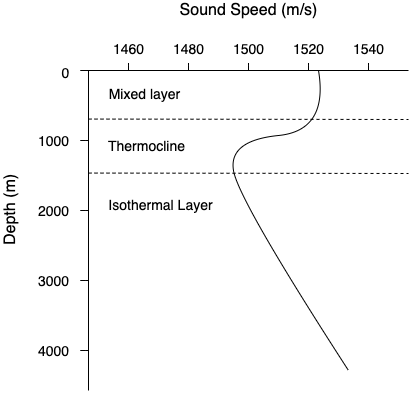
\includegraphics[width=0.6\textwidth]{figures/sound-profile}
	\caption{Generic sound speed profile}
	\label{fig:spd-sound}
\end{figure}

The empirical equation \ref{eq:spd-sound} \cite{ocean-acoust} is a simplified translation of the behavior of the sound speed \textit{c} in meters per second, with relation to the temperature \textit{T} in ºC, the salinity \textit{S} in parts per thousand and the depth \textit{z} in meters. 
\begin{eqnarray}
c = 1449.2 + 4.6T - 0.055T^2 + 0.00029T^3 + (1.34 - 0.01T)(S-35) + 0.016z 
\label{eq:spd-sound}
\end{eqnarray}


\subsection{Multipath} \label{subsec:multipath}

Multipath occurs when a transmitting signal suffers reflection or refraction in a surface (e.g. water surface, ocean floor, dock's wall), leading to a change in its original characteristics. This phenomenon can affect the propagation speed, the energy and the total distance that the signal was predicted to travel. These altered signals in conjunction with constant movement of the receiver makes it more complicated to accurately estimate the distance between the transmitter and the receiver, as well as determine the line-of-sight signal. 

\begin{figure}[!htbp]
	\centering
	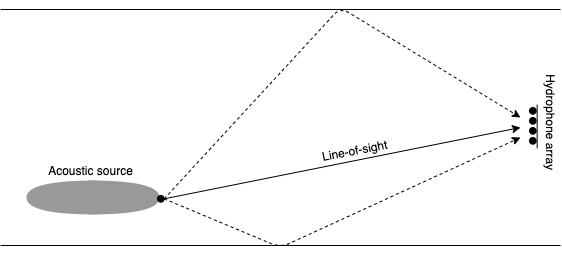
\includegraphics[width=0.7\textwidth]{figures/multipath}
	\caption{Multipath}
	\label{fig:mpath}
\end{figure}

In consequence, the underwater acoustic channel is qualified as a non-minimum phase system because it produces time-variant output responses.

\subsection{Doppler Effect} \label{subsec:doppler}

In a communication and localization system between two entities moving with non-zero relative velocity, if a transmitter sends a signal with a certain operation frequency to the receiver, then the perceived frequency by the receiver will suffer a shift from the original signal. This frequency difference is expressed as a Doppler shift and explained by the Doppler Effect.

The magnitude of the generated frequency shift can be expressed as a ratio \ref{eq:ratio}, where the transmitter-receiver velocity is compared to \(c\), the speed of sound \cite{commchan}.

\begin{eqnarray}
&a = \frac{v}{c}
\label{eq:ratio}
\end{eqnarray}

Autonomous Underwater Vehicles (AUVs) usually move with velocities in the order of few meters per second. Therefore, the \(a\) factor mentioned above has a significant value and needs to be considered when implementing synchronization systems, as well as developing estimation algorithms.

In certain localization and communication systems, it is critical to correct the Doppler effect because data can be compromised (e.g. FSK modulated signals, in which information is codified into frequency changes). A simple Doppler compensation process  was proposed in \cite{thesis-joao}, in a system to detect phase-modulted binary sequences using cross-correlation.

This phenomenon can also be explored to determine the relative velocity between two devices, by measuring the frequency deviation with respect to the frequency expected to be received.


\subsection{Attenuation and signal-to-noise ratio} \label{subsec:snr}

When considering underwater communication systems, it is essential to quantify the attenuation of the channel, i.e. the part of the signal's energy which is absorbed by the involving surrounding. In underwater channels, this absorbance is frequency variable and it is also dependent on physical characteristics of the water, as salinity and temperature. 

The underwater acoustic channel has a particular model that describes its attenuation path loss \(A(d,f)\), given in logarithmic scale by equation \ref{eq:attenuationdb} \cite{pathloss}. 
\begin{eqnarray}
&10\ log(A(d,f)) = 10\ k\ log(d) + d\ 10\ log(a(f))
\label{eq:attenuationdb}
\end{eqnarray}
From the equation, \(d\) is the distance from the transmitter to the receiver in kilometers (Km), \(f\) is the operating frequency in kilohertz (KHz), \(10klog(d)\) represents the spreading loss which describes how the sound level (in decibel, dB) decreases as the sound wave spreads, \(d10log(a(f))\) is the absorption loss that a signal suffers during its propagation path, \(k\) is the spreading factor which is related with the considered configuration (e.g. cylindrical, spheric, etc.), \(a(f)\) is the absorption coefficient that can be obtained through the equation in \cite{pathloss}.

Noise is another factor that is considered when analyzing a real underwater acoustic channel, as it defines the signal-to-noise ratio (SNR) that characterizes the channel. The SNR is dependent on the attenuation level which increases with frequency, and the noise which decays with frequency. Consequently, the SNR varies over the signal bandwidth and it is asymmetric. The equation \ref{eq:snr} \cite{commchan} expresses this relationship, where \(S_{d}(f)\) represents the power spectral density of the transmitted signal.
\begin{eqnarray}
&SNR(d,f) = \frac{S_{d}(f)}{(A(d,f))\ N(f)}
\label{eq:snr}
\end{eqnarray}

%________________________________________________________

\section{Range estimation for underwater localization}

Underwater localization takes into consideration the distance between the target object to track and the reference point. As consequence, it is always relevant to apply methods which easily and effectively determine this range.

There are two main types of techniques that are used to achieve such objective: the Received Signal Strength Indicator (RSSI) and the Time Delay Estimation (TDE).


\subsection{Received Signal Strength Indicator}

The Received Signal Strength Indicator (RSSI) method is based on the strength of the signal that reaches the target. It determines the distance between the target and the reference node by analyzing the received signal strength and comparing it with an underwater attenuation model which is range dependent \cite{ocean-acoust}. 

Since the underwater acoustic channel suffers from multipath, time variance and high overall path loss, the RSSI technique is not adequate for underwater applications.

\subsection{Time Delay Estimation}
Time Delay Estimation (TDE) mechanisms use a pair of nodes, the target and the reference point, to measure the range between them. This distance is based on the time that it takes for a signal to travel from the reference point to the target.

There are three main categories that devide TDE methods, which are Time Difference of Arrival (TDOA), Time of Arrival (TOA) and Time of Flight (TOF).

\subsubsection{Time of Arrival}

Time of Arrival (TOA) is interpreted as the time delay between the transmission of a signal in the reference node until its reception on the target node. Although this is the conceptually simplest method to employ, it requires synchronization between the nodes since the target entity needs to know the instance when the signal was sent to be able to calculate the difference.

Considering a generic transmitted signal \textit{s(t)}, the received signal can be expressed as \ref{eq:toa}, where $\tau$ represents the time of arrival and \textit{n(t)} is white noise with zero mean \cite{wirelesscomm}. 

\begin{eqnarray}
& r(t) = s(t - \tau) + n(t)
\label{eq:toa}
\end{eqnarray}

\subsubsection{Time Difference of Arrival}

The Time Difference of Arrival (TDOA) is a technique that compares the time of arrival of a signal to different hydrophones in order to estimate the angle of arrival of the acoustic signal. The array of reception hydrophones have known determined positions among them so that is is possible to compare the different times of arrival or phase differences. This method can be employed using a uni-directional signal or a round trip communication.

There are several algorithms and mathematical models that can be employed to execute the TDOA method, such as the Cross-Correlation and Maximum Likelihood.

\subsubsection{Generalized Cross-Correlation}

The Generalized Cross-Correlation (GCC) method is used to generically represent the relationship strength between two signals.

Considering two distanced hydrophones in the same environment and an acoustic source \textit{s(t)}, \textit{x1(t)} and \textit{x2(t)} are the signals received by each of the two hydrophones. The equations \ref{eq:gcc1} and \ref{eq:gcc2} \cite{crosscorr} express the mentioned signals in relation to \textit{w1(t)} and \textit{w2(t)} which are Gaussian noise coefficients uncorrelated with the source, $\tau$ that represent the delay and $\alpha$ which is an attenuation function.
\begin{eqnarray}
&x1(t) = s(t) + w1(t)
\label{eq:gcc1}\\
&x2(t) = \alpha s(t - \tau) + w2(t)
\label{eq:gcc2}\\
\end{eqnarray}

From these expressions, the generalized cross-correlation function between signals \textit{x1(t)} and \textit{x2(t)} is given by \ref{eq:gcc3}. The $G_{x1x2}(f)$ is the spectrum of the cross-correlation. The $\psi(f)$ represents a prefilter and it is essentially the distinctive parameter that originate various different methods of cross-correlation, since it should depend on different environments and properties as SNR. 
\begin{eqnarray}
& R_{x1x2}(\tau) = \int_{-\infty}^{\infty} \psi(f) G_{x1x2}(f)\ e^{i2\pi f\tau} df
\label{eq:gcc3}\\
& T = \tau_{max} [ R_{x1x2}(\tau) ]
\label{eq:gcc4}
\end{eqnarray}

Finally, the maximum value of $R_{x1x2}(\tau)$, expressed in \ref{eq:gcc4}, is the so called correlation peak and provides information about the time delay $\tau$ which is the main matter of Time Delay Estimation. 


\subsubsection{Cross-Correlation}

After approaching the generalized method of cross-correlation, it is possible to better understand the Cross-Correlation (CC) method. There are two main variations of CC \cite{crosscorr}, which are the slow cross-correlation in the  time domain and the fast cross-correlation in the frequency domain. The second approach is based on the Fast Fourier Transform as it locates the peak by analyzing frequency similarities between the signals. 

Th Cross-Correlation technique uses a prefilter $\psi(f)$ equal to 1, as it is the simplest method of its kind.

\subsubsection{Maximum Likelihood}

The Maximum Likelihood (ML) method is a variation of Cross-Correlation which uses the prefilter $\psi(f)$ represented mathematically by \ref{eq:ml1}, where $\gamma_{12}(f)$ is a function of spectrum of cross-correlation $G_{x1x2}(f)$ and spectrum of auto-correlations $G_{x1x1}(f)$, $G_{x2x2}(f)$ as expressed in \ref{eq:ml2} \cite{crosscorr}.

\begin{eqnarray}
& \psi(f) = \frac{|\gamma_{12}(f)|^2}{|G_{x1x2}(f)|[1-|\gamma_{12}(f)|^2]}
\label{eq:ml1} \\
& |\gamma_{12}(f)|^2 = \frac{|G_{x1x2}(f)|^2}{G_{x1x11}(f) . G_{x1x11}(f)]}
\label{eq:ml2} 
\end{eqnarray}

There is also a version of ML that uses the power spectral densities of the signals, which can be helpful for calculations in various applications. 

\subsubsection{Time of Flight}

Time of Flight (TOA) measures essentially the round-trip time communication between two nodes. The target node sends a signal to the reference node, which has an integrated transponder that responds transmitting a signal back to the target. T4he TOA is then estimated as the time interval from the moment the first signal is transmitted until the moment the second signal is received by the same node. 

This method may be used without additional synchronization systems as it assumes that the response signal is sent immediately after the received one and the intrinsic transmitting delays are known.

The accuracy of this technique depends mainly on the environment conditions, which include the water properties and the surrounding reflection surfaces which cause multipath. Therefore, the mechanism is susceptible of variable errors according to the location and characteristics of its employment.

%________________________________________________________

\section{Localization estimation}

In networks with multiple nodes is typical to use localization estimation to establish position relationships between elements. The operation principal is usually to have a set of reference nodes with known positions so that it is possible to determine the relative positions between each reference node and the target. 

An extensive comparison of different localization schemes for underwater sensors networks can be consulted in \cite{suvey-loc}.

\subsection{Triangulation}

Triangulation is a method of localization based on the measurement of angles which are related to the reference beacons and the target object. 

\subsubsection{Three-Object Triangulation}
The simplest method of this category is the Three-Object Triangulation, which considers a configuration as illustrated in figure \ref{fig:tri1}. It is assumed that the location of the beacons is pre-configured and the environment is obstacle-free. $\lambda_{12}$ is the angle formed by the intersection of the straight lines [O,1] and [O,2]. Similarly, $\lambda_{31}$ is the angle formed by the intersection of the straight lines [O,1] and [O,3]. Using these two sets of nodes, we can trace circumferences that include their coordinates and as a consequence their intersection will correspond to the location of the target.

\begin{figure}[!htbp]
	\centering
	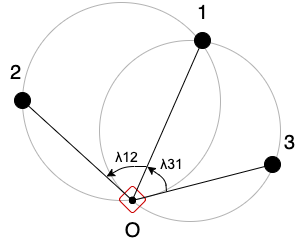
\includegraphics[width=0.4\textwidth]{figures/triangulation}
	\caption{Three-Object Triangulation}
	\label{fig:tri1}
\end{figure}

Although this is a very straightforward technique to implement, it does not cover all possible scenarios, namely when the three beacons and the object are all placed in the same circumference or when the environment has obstacles between nodes.

\subsubsection{Geometric Triangulation algorithm}

A more complex method relies on the Geometric Triangulation algorithm. 

\begin{figure}[!htbp]
	\centering
	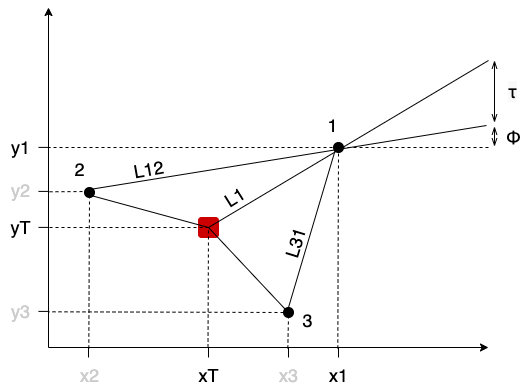
\includegraphics[width=0.5\textwidth]{figures/geotriang}
	\caption{Geometric Triangulation algorithm}
	\label{fig:tri2}
\end{figure}


Considering a Cartesian plane with defined lengths L1, L12 and L31, as shown in image \ref{fig:tri2}, it is possible to establish trigonometrical relationships that estimate the location of the object within the created triangular areas. The position of the target is given by coordinates (xT,yT) and can be calculated through equations \ref{eq:tri1} and \ref{eq:tri2}. (x1,y1) represents the location of beacon 1 and L1 is the distance between this beacon and the object. The trigonometric relationships for calculating the mentioned variables can be consulted in \cite{triangalgo}.

\begin{eqnarray}
& xT = x1 - L1 * cos(\phi + \tau)
\label{eq:tri1}\\
& yT = y1 - L1 * sin(\phi + \tau)
\label{eq:tri2}
\end{eqnarray}

\subsection{Trilateration}

Trilateration is a technique that does not rely on calculations using angles but instead it uses distances to locate an object.

Considering a scenario with three reference beacons, the distance between the target and each one of the beacons is taken as the radius of a circumference. By doing this, it is possible to obtain three circumferences that intersect each other. With only two circumferences, there are two possible locations for the object, however, when added the third circumference the exact location is obtained. The 2D coordinates are obtained by solving systems of equations with the circle equation \ref{eq:circle} \cite{trilat}, where $(x_{i}, y_{i})$ is the beacon coordinates and $r_{i}$ is the distance between the beacon and the object.

\begin{eqnarray}
& (x - x_{i})^2 + (y - y_{i})^2 = r_{i}^2 
\label{eq:circle}
\end{eqnarray}

Trilateration is commonly used in underwater acoustic localization, as it used to find a relative position of the target in two dimensions and additionally determines the depth as third dimension, by using a pressure sensor with high accuracy.

\subsection{Multilateration}

Multilateration is a generalization of the trilateration technique, as it uses the same conceptual principal with multiple reference beacons instead of exactly three. In this method, the employment of \textit{n+1} nodes will allow to determine \textit{n} coordinates \cite{arch_localiz}. For example, determining the position (x,y,z) of a target, would require to resolve a system of equations using \ref{eq:mult}. $(x_{i}, y_{i}, z_{i})$ is the coordinates of the beacon and $d_{i}$ is the distance between the beacon and the target.

\begin{eqnarray}
& (x - x_{i})^2 + (y - y_{i})^2 + (z - z_{i})^2 = d_{i}^2 
\label{eq:mult}
\end{eqnarray}

Distributed mechanisms, such as multilateration, are usually divided in three phases of positioning \cite{suvey-loc}:
\begin{itemize}
	\item Distance estimation between the reference nodes and target object, usually using TDOA or TOF mechanisms;
	\item Position estimation, usually obtained by solving a system of linear equations through mathematical efficient techniques;
	\item Final refinement of the measurement in order to improve accuracy.
\end{itemize}

As an alternative to solve localization issues using circumferences, multilateration can also take advantage of a hyperbola-based localization method. Considering a target at (x,y) and three reference beacon with coordinates $(x_{i},y_{i})$,  $(x_{j},y_{j})$ and  $(x_{k},y_{k})$, we have that the difference between times of arrival $t_{i}$ and $t_{j}$ to nodes $i$ and $j$, respectively, can be related to the distance between nodes, as expressed in \ref{eq:hyper} \cite{arch_localiz}. $d_{i}$ and $d_{j}$ are the distance from node $i$ and $j$, respectively, to the target object. 

\begin{eqnarray}
& d_{i} - d_{j} = c * (t_{i} - t_{j}) = \sqrt{(x - x{i})^2 + y - y{i})^2} - \sqrt{(x - x{k})^2 + y - y{k})^2}
\label{eq:hyper}
\end{eqnarray}

%________________________________________________________

\section{Positioning Systems}

Positioning systems are used to track the underwater position of a vehicle or other object, in relation to reference structures of transponders called \textit{baseline stations}. These systems are classified based on the distance between the baseline stations. The configurations that will be explained are Long Baseline (LBL), Short Baseline (SBL), Ultra Short Baseline (USBL) and the inverted versions of all above.

\begin{figure}[!htbp]
	\centering
	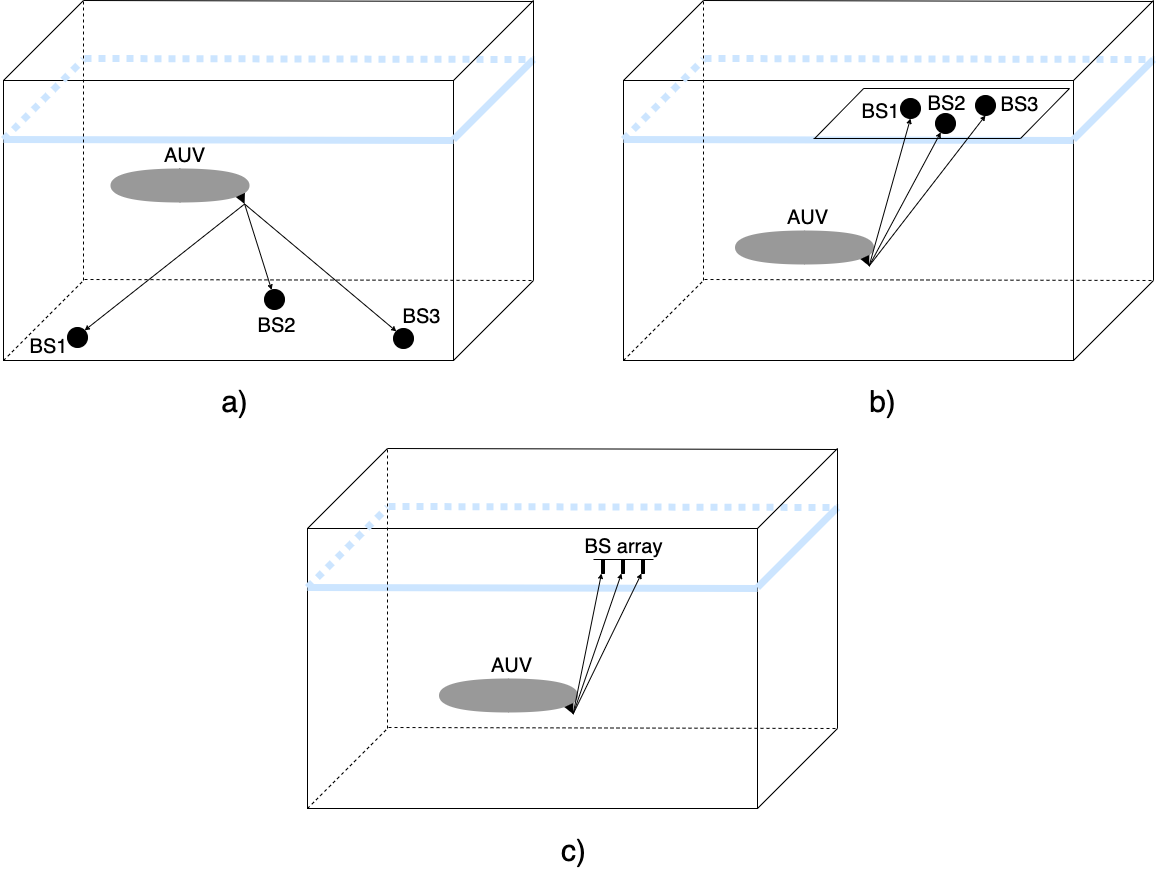
\includegraphics[width=1\textwidth]{figures/lblsblusbl}
	\caption{Generic configuration of: a) LBL; b) SBL; c) USBL}
	\label{fig:lblsblusbl}
\end{figure}

\subsection{Long Baseline (LBL)}

Long Baseline systems use a positioning method with large distances between baseline stations, with range typically from 50m to more than 2000m  and usually similar to the distance between object and transponders \cite{crosscorr}. A typical LBL configuration is represented in figure a) \ref{fig:lblsblusbl}.

The LBL method uses at least three transponder stations deployed usually on the sea floor, allowing to execute trilateration. Additionally, a transducer is integrated on the object to be tracked. 

A complete localization procedure starts with the vehicle sending an acoustic signal which is received by the transponders. Thereafter the transponders transmit a response and, by analyzing the Time of Flight of the communication, the system can determine the distance between the vehicle and each base station. Then the relative position of the vehicle is determined through trilateration. Additionally, if the transponders have known geographic positions, it is possible to infer the vehicle geographic position. 

As this technique presents large distances between the object and the base stations, the typical 1m to few centimeters accuracy is considered to be high because it will not compromise the localization of the vehicle. 


\subsection{Short Baseline (SBL)}

Short Baseline systems are characterized by having distances around 20m to 50m between baseline stations \cite{survey-tech-chall} and use an operation procedure similar to the LBL method. However, the transponders are usually placed in a moving platform, which assures a fixed relative position between them. A typical SBL configuration is represented in figure b) \ref{fig:lblsblusbl}.

The position of the vehicle to be tracked can be determined by translating the Time of Flight between the multiple transponders and the object into a distance value, which is achieved by equation \ref{eq:sbl} \cite{sbl}. The $t_{i}$ corresponds to the propagation time of the signal from the vehicle to the \textit{i}th transponder, \textit{c} is the speed of sound, [$x_{b_{i}}$, $y_{b_{i}}$ and $z_{b_{i}}$] is the coordinate position of the transponder.

\begin{eqnarray}
&\sqrt{ (x_{b_{i}}-x)^2 + (y_{b_{i}}-y)^2 + (z_{b_{i}}-z)^2 } = c\ *\ t_{i}
\label{eq:sbl}
\end{eqnarray}

In a SBL system, when the distance between baseline stations is increased the accuracy improves and, contrarily, when the mentioned distance decreases the accuracy deteriorates, which can raise some deployment challenges.

\subsection{Ultra Short Baseline (USBL)}

Ultra short baseline systems are composed essentially by one baseline station, with an array consisting of several traducers distanced typically less than the wavelength \cite{lblsblusbl}, and a transponder integrated on the object to be tracked. It is usually used in underwater positioning in shallow areas of the sea, as represented in figure c) \ref{fig:lblsblusbl}.

Similarly to the previously mentioned procedures, the USBL positioning method relies on the Time of Flight of the exchanged signals. However, the traducers are too spatially close from each other to execute an accurate trilateration. Instead, it is measured the phase difference or time-delay difference of the received signal between every traducer, in order to estimate the azimuth and distance to the acoustic source. 

Assuming a three dimensional scenario for the positioning system, as represented in figure \ref{fig:usblgeo}, the object's coordinates are given by equations \ref{eq:usblgeo1}, \ref{eq:usblgeo2} and \ref{eq:usblgeo3} \cite{usbl-new}. The $\lambda$ corresponds to the wavelength of the of the transmitted signal which depends on its operation frequency, \textit{f}, and it is affected by the speed of sound \textit{c}, as represented equation \ref{eq:cfw}.
The \textit{d} represents the distance between hydrophones, $\psi_{12}$ and $\psi_{22}$ are the phase difference between H2 and the other two hydrophones, \textit{H} is the height of the target object, \textit{X} is the distance of the target along the x-axis direction, \textit{Y} is the distance of the target along the y-axis direction and \textit{l} is the slant distance of the target to the hydrophone.
\begin{eqnarray}
& c = f * \lambda
\label{eq:cfw}
\end{eqnarray}
\begin{eqnarray}
& l^2 = X^2 + Y^2 + H^2 
\label{eq:usblgeo1}\\
& \psi_{12} = \frac{2\pi}{\lambda}[\sqrt{l^2} - \sqrt{(d-X)^2 + d^2 + H^2}]
\label{eq:usblgeo2}\\
& \psi_{22} = \frac{2\pi}{\lambda}[\sqrt{l^2} - \sqrt{X^2 + (d-Y)^2 + H^2}]
\label{eq:usblgeo3}
\end{eqnarray}

\begin{figure}[!htbp]
	\centering
	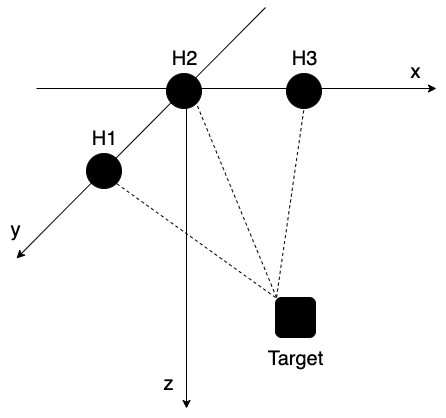
\includegraphics[width=0.5\textwidth]{figures/usbl-config}
	\caption{USBL system configuration}
	\label{fig:usblgeo}
\end{figure}

This is a broadly used technique due to its convenient set up, which allows to have predefined measurements in the order of tens of centimeters and does not require AUV navigation area for the deployment. However it presents the lowest accuracy, comparatively with LBL and SBL, since an error of few centimeters can be realistically corresponding to an inaccuracy of several meters in the position of the object to be tracked.

\subsection{Inverted Systems}

All the previously mentioned positioning techniques use a configuration in which the vehicle to be tracked has a single transducer and there is an external set of transponder to determine the positioning of the said object. However, there is the possibility to benefit from the inverse configuration in some applications. Therefore, there are also the iLBL, iSBL and iUSBL methods, which have the same operation principals as LBL, SBL and USBL, respectively.

%_________________________________________________________


\section{Commercial Solutions}

There are several commercial solutions for underwater positioning using the ultra-short baseline method. In this section, it will be presented some of the available devices in the market, indicating their main properties and capabilities. Table \ref{tab:solutions} summarizes the systems with most relevance to the present work. The Medium Frequency (MF) bandwidth is attributed to devices whose manufacturer did not specified the actual frequency range.

\textit{Evologics} produces the S2C R USBL series of acoustic modems \cite{evologics1}, with Sweep Spread Carrier (S2C) technology \cite{evologics2} which uses a broad frequency range to propagate over large distances with reduced noise. The devices have a fixed 0.01m slant range accuracy and a 0.1 degree bearing resolution. These are essentially divided into two groups:
\begin{itemize}
	\item High speed mid-range devices: contains the 18/34 transceivers family \cite{evologics3}, which presents various options for the USBL antenna beam pattern and it is optimal for transmission in horizontal channels.
	\item Depth rated long-range devices: includes the 12/24 transceiver \cite{evologics4}, which have a directional (70 degrees) USBL antenna  and it is optimal for transmission in vertical channels.
\end{itemize}

\textit{Sonardyne} markets the Ranger 2 systems. The Micro-Ranger 2 \cite{sonardyne1} is very easy to use without previous experience and it is appropriate for shallow waters, achieving accuracy of 0.2\%. The Mini-Ranger 2 is ideal for nearshore missions and it is  used for simultaneous tracking of various mobile targets, whose position is updated every 3 seconds.

\textit{Applied Acoustics} offers the Easytrak USBL Systems, which includes the processing software for estimating the position. The Alpha Portable 2655 consists in a very compact structure that includes an array transducer and is capable of reaching a 10cm slant range resolution and a 2 degree RMS.

\textit{Kongsberg} produces the HiPAP family of transducers \cite{hipap_hardw}, which can use the Cymbal acoustic protocol (PSK) or the frequency shift (FSK) modulation technique. Particularly the HiPAP 352 is the model with higher number of active transducers and is able to reaches 0.02m of range accuracy.

\begin{table}[H] %use !htbp to adjust
	\begin{tabular}{|c|c|c c c|}
		\hline
		Company
		& System
		& Bandwidth(kHz)
		& Connection(kbps)
		& Range(m) \\ \hline 
		\multirow{2}{4em}{Evologics} 
		& S2C R 18/34D USBL & 18-34 & up to 13.9 & 3500\\
		& S2C R 12/24 USBL & 12-24 & up to 9.2 & 6000\\
		\hline 
		\multirow{2}{4em}{Sonardyne} 
		& Micro-Ranger 2 & MF & 0.2-9 & 995\\
		& Mini-Ranger 2 & MF & 0.2-9 & 995\\ 
		\hline 
		\multirow{2}{4em}{Applied Acoustics} 
		& Easytrak Alpha Portable 2655 & MF & n.d. & 500 \\
		&  &  &  & \\
		\hline 
		\multirow{1}{4em}{Kongsberg} 
		& HiPAP 352 & 21-31 & n.d. & 5000 \\
		\hline 
	\end{tabular}
	\caption{Overview of commercial solutions}
	\label{tab:solutions}
\end{table}

% http://www.teledynemarine.com/usbl-dat?ProductLineID=59
% https://www.link-quest.com/html/tl10000.pdf
% https://www.tritech.co.uk/product/usbl-tracking-system-micronnav

%_______________________________________________________________________________

\section{Angle of arrival determination}

\section{Methods for optimizing sensor configurations }

When evaluating the performance of a localization system which integrates a multiple sensor configuration, it is essential to resort to widely used methodologies to prove its validity and accuracy. This section is dedicated to explore some commonly employed methodologies.

\subsection{Crámer-Rao lower bound}	\label{sec:cramer}

In this thesis, it is conducted a study based on the Crámer-Rao lower bound, which is generally used to generate a \textit{so-called uncertainty ellipse} \cite{bishop-cramer-rao} that represents the spatial variance distribution of the estimated position. The overall desired result is to find the minimum variance value that is related to the chosen configuration geometry, which indicates that it is the optimal solution for estimating a certain position. This method utilizes the Fisher Information matrix (FIM), whose components translate characteristics of the observation vector.

In order to avoid loss of generality, it is considered a set of N sensors and a settled position for the target, the acoustic source, defined by $s_{t}$ = [$x_{s_{t}}$, $y_{s_{t}}$, $z_{s_{t}}$]$^T$. In addition, the position of each sensor is defined as $r_{i}$ = [$x_{r_{i}}$, $y_{r_{i}}$, $z_{r_{i}}$] and, consequently, the measurement of distance between each sensor and the source is defined as d$_{i}$ = $|| s_{t} - r_{i} ||$.

Thereafter, the observations vector will be formulated containing the observed times-of-arrival (TOA) of the signal from the acoustic source to each one of the hydrophones, considering their geometric position. These times contain a noise vector component, which can be approximated to to a Gaussian distribution $n_i \sim \mathcal{N}(\mu,\,\sigma^{2})$. The samples can be calculated through the expression \ref{eq:obs_vec}, where it is considered an initial time of arrival $t_0$. Additionally, c represents the sound speed underwater.

{\large\[
	t_i = t_0 + \frac{||d_i||}{c} + n_i
	\label{eq:obs_vec}
	\]}

After having the observations matrix, it is established the condition to formulate the Fisher Information matrix, $I(d)$ , which results into equation \ref{eq:fisher}.

{\large\[
	I(d) = \nabla_{d}t(d)^T \; \Sigma^{-1} \; \nabla_{d}t(d)
	\label{eq:fisher}
	\]}

$\nabla_{d}t(d)$ is the gradient matrix of the observations vector regarding $d_i$, whereas $\Sigma$ is the covariance matrix, in which the diagonal contains the standard deviation of the components of each noise vector, construed as $(\sigma_1^2 , \sigma_2^2 , ... , \sigma_N^2)$ .

Thereby, all conditions are established to proceed to the actual calculation of the Fisher Information matrix. After formulated, it will indicate the quantity of information that a certain sensor configuration can give about a position in space. Hence the goal is to obtain the maximum achievable information. By calculating the determinant of FIM it is possible to deduce the minimum \textit{uncertainty ellipsoid} and therefore the configuration's best possible performance. Therefore, the optimal solution is given by the maximum output of the determinant of FIM.

Additionally, it is possible to detail this information by calculating the actual size of the axis that compose the \textit{uncertainty ellipsoid}. This is achieved by calculating the square mean root of the eigenvalues of $I(d)$, which correspond to each axis size.

Further explanation about the methods used in a deeper exploration of the Crámer-Rao lower bound can be consulted in \cite{bishop-cramer-rao}, which serves as guide to investigate other scenarios of application of this theorem. However, the mentioned concepts were all the necessary for the approach on this dissertation .

This same process is adopted in this dissertation. All steps specifically taken for this study are declared in section \ref{sec:config-perf} of the present document.

%_______________________________________________________________________________
%_______________________________________________________________________________


\chapter{Digital Signal Processing } \label{chap:hdl}

In order to implement the USBL system, a custom digital signal processing system has been implemented to compute in real-time the time differences of arrival of the acoustic signal arriving to the hydrophone array. The system was implemented in a FPGA-based platform and included in a previous signal processing system that determines the time of arrival of an encoded acoustic signal by implementing an efficient time-domain cross correlation. 

This chapter introduces the process to calculate the time differences of arrival by combining the results of the cross-correlation with the differences of phase between the signals received by the different hydrophones.

\section{TDoA Estimation}

To improve the determination of the time difference of arrival between the hydrophones, the implemented signal processing system calculates the difference of phase between the received signals. As the distance between hydrophones, i.e. the baseline, is always larger than the wavelength of the acoustic signals used, the phase alone is not sufficient to determine the time difference of arrival. Time-domain correlation is thus combined with the phase difference calculation to remove the ambiguity and obtain a time difference of arrival with a time resolution that is far beyond the sampling period used in the digital signal processing system.

When the information about the time of arrival of a signal is available, it is relatively easy to estimate the distance between the transmitter and the receiver since there can be a direct conversion between them. However, when dealing with phase differences, there is no exact time notion, so it is necessary to start by defining a reference point. 

Considering sinusoidal signals, when we have an array with four hydrophones spatially placed to form a 3D layout, the signal that is arriving to each  hydrophone in different times consequently have different phases. However, since sinusoidal signals are periodic, this means that for different signal periods the same phase value is observed, i.e. the phase is ambiguous \ref{fig:phasediff}. In this illustration, $\alpha$ represents the observable phase difference of hydrophone $H_4$ to the reference point $H_1$. However, the actual time difference which is intended to obtain, $\Delta t_4$, is one period of the signal, $\lambda$, added to the observable phase $\alpha$.

\begin{figure}[!htbp]
	\centering
	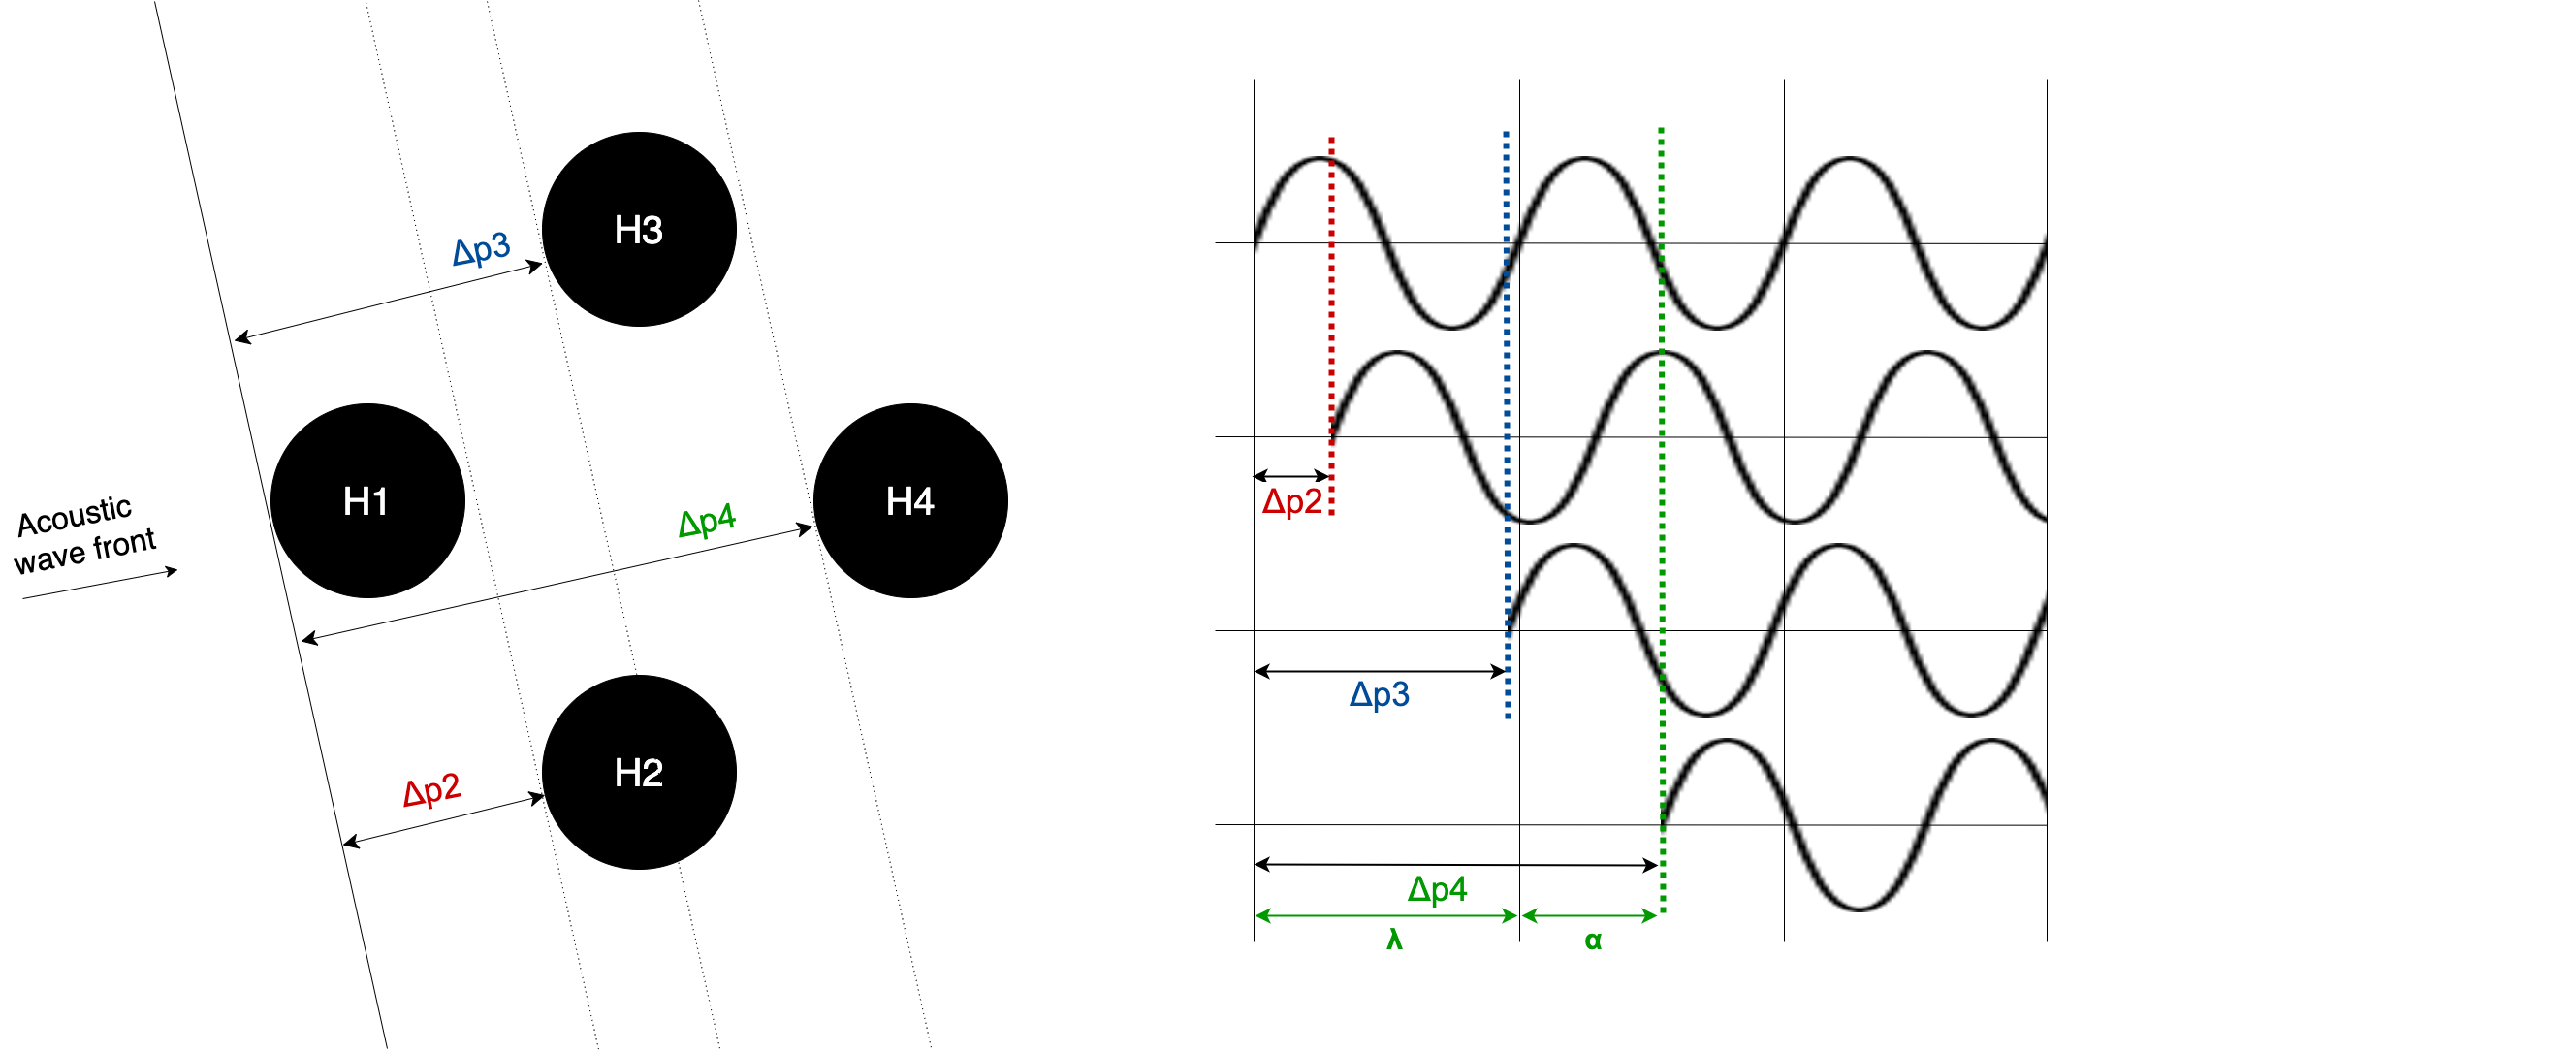
\includegraphics[width=1.2\textwidth]{figures/phase-diff}
	\caption{Phase difference to reference point and phase ambiguity}
	\label{fig:phasediff}
\end{figure}

For this reason, it is crucial to consider that the phase difference is given by the obtained phase value added by the number of periods ahead from the considered reference period.

In the system under study, the transmitted signal is a pure sine wave with a frequency of 24.4 $kHz$. The corresponding signal period is $T = \frac{1}{24400} $ seconds which, considering the typical underwater acoustic speed $c_s$ equal to 1500 $m/s$, the wavelength is approximately equal to $\lambda = \frac{T}{c_s} = 6.1 cm$. Having this into consideration, after obtaining the time of arrival to each hydrophone given by the cross correlation instances, besides the reference one, it is possible to conclude if the phase shift is superior to one period by analyzing if the time difference is greater than the duration of one period $T$. In figure \ref{fig:phasediff}, each mentioned time difference $\Delta t_2$, $\Delta t_3$ and $\Delta t_4$, between $H_1$ and $H_2$, $H_3$ and $H_4$ is converted to the corresponding phase differences.

One possibility to solve phase ambiguity in this system would be to place the four hydrophones with a baseline spacing inferior to $\frac{1}{2}$ of a wavelength, since the maximum reached by phase difference is 180 degrees. This way it would be possible to immediately deduce the phase difference since it would always be contained in one period. However, positioning the hydrophones closer together leads to smaller  values, causing an increase on the estimation error due to varying environment conditions (briefly enumerated in \ref{subsec: acoustic-channel}). Additionally, since the hydrophones to be used in this system have a corresponding diameter of roughly half of a wavelength, they would not allow to execute the mentioned configuration and so this possibility will not be contemplated.

In order to compensate this phase ambiguity, a simple relation was developed which allows to calculate the absolute time difference between the moment a signal is received by hydrophone A, $T_A$, and when the same signal is received by a further hydrophone B, $T_B$. Figure \ref{fig:ambiguity} illustrates this association, where the represented sinusoidal waves correspond to the same signal arriving at hydrophones A and B. 

\begin{figure}[!htbp]
	\centering
	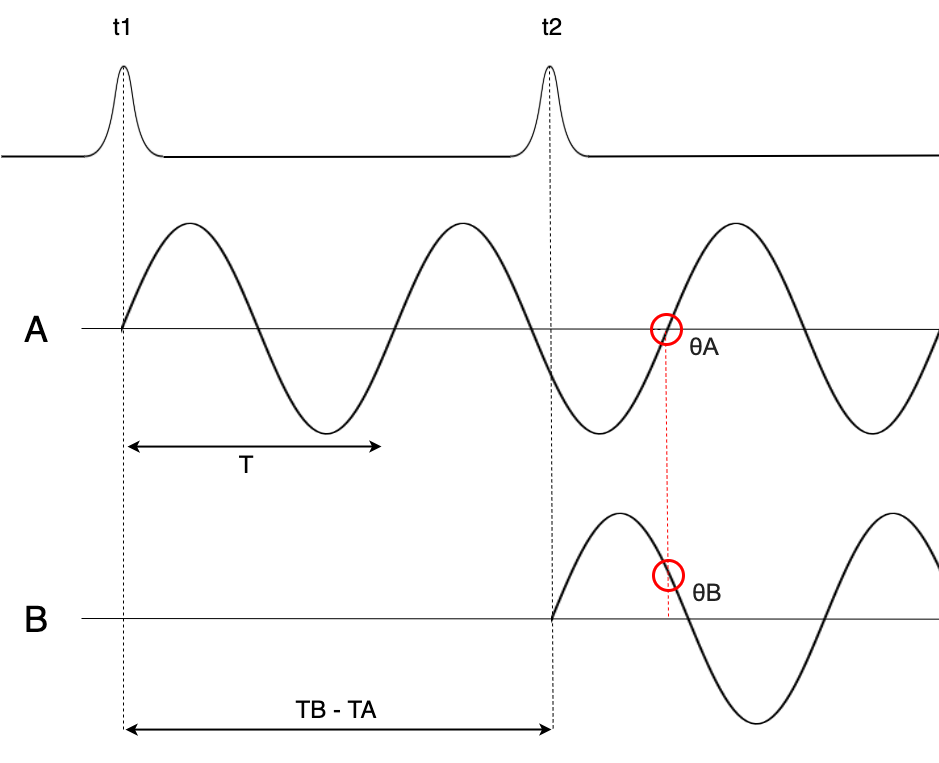
\includegraphics[width=0.6\textwidth]{figures/ambiguity}
	\captionsetup{justification=centering,margin=2cm}
	\caption{Ambiguity correction through correlation and phase difference}
	\label{fig:ambiguity}
\end{figure}

This correspondence uses the time stamps obtained by the correlation peaks combined with the calculated phase difference, that is determined in parallel, so that the measurement is more accurate. Equation (\ref{eq:phase-amb}) translates this relation, where $t_1$ and $t_2$ are the correlation peaks obtained from the signal arriving at hydrophone A and B, respectively, and so by rounding for the next integer number the difference between the correlation peaks, $t_2 - t_1$, we will obtain in which period, $T$, of signal in A will the signal in B arrive. Then the measurement is improved by subtracting a phase difference, $\theta_B - \theta_A$, so that the instant at which the signal is detected in hydrophone B can be defined. 

\begin{eqnarray}
	& T_B - T_A = round(\frac{t_2-t_1}{T}) - (\theta_B - \theta_A)
	\label{eq:phase-amb}
\end{eqnarray}

\section{HDL Module Architecture} \label{subchap:HDL module}

In a previous dissertation project \cite{afonso-thesis}, a signal processing system has been implemented to determine the time difference of arrival of an acoustic signal to a set of 4 hydrophones. This system is based on the transmission of a known binary sequence modulated in PSK (Phase Shift Keying) and the detection of the signal received by performing an efficient time-domain cross-correlation between the signals received at each hydrophone and the transmitted signal. The system was intended to determine the 3D position of an acoustic source in a confined structured space, where the 4 hydrophones were distanced a few meters between them. The implemented correlation process allow to obtain the time of arrival of the sound wave with a timing resolution equal to one sampling period that corresponds to a distance resolution approximately equal to 6 mm, which has been considered enough for the spacial accuracy of the 3D positioning system.

The current work intends to enhance that system to improve the accuracy of the calculation of the time differences of arrival. This is achieved by computing in real time the phase differences between the signals arriving to each hydrophone and combining that with the time of arrival calculated by the correlation process. The objective of this system is to implement a Ultra-Short Base Line (USBL) underwater localization system to estimate the 3D angle of arrival of the acoustic signal, for integration in a small Autonomous Underwater Vehicle (AUV). Due to the relatively small size of the AUV, the 4 hydrophones will have to be separated by the maximum of a few tens of centimeters. Therefore, the maximum resolution in distance that is possible to obtain with the correlation process alone is not enough for accurately determining the angle of arrival. Preliminary experimental results have showed that, with the phase analysis combined to the cross-correlation, the time differences may be obtained with an accuracy corresponding to a distance below one millimeter. 

To implement this process, that acoustic source transmits a sinusoidal signal with a know fixed frequency (24.41 kHz) after the BPSK encoded signal used by the correlation process. The phase analysis mechanism makes use of this signal which is know to appear a fixed time after the detection of the encoded signal.

\subsection{Module Components}

The overall system is composed by four main functional blocks, represented in \ref{fig:module-all}. The hydrophone array, composed by hydrophones $i$ with $i=\{1,2,3,4\}$, receives the signals in each sensor and sends them to an Analog to Digital Converter (ADC). The generated digital signals are then input of a module based on a Hilbert transform, which converts the real signals to their complex representation. These are then multiplexed so each pair of real, $Re_i$, and imaginary, $Im_i$, components are input in a CORDIC \cite{cordic-def} block, responsible for computing the signal's phase, $phase_i$. Afterwards, the phase differences $phdiff_{ij}$ are calculated for all the combinations of two hydrophones and finally they are averaged in order to obtain a more stable phase difference, $\Delta phase_{ij}$.

The module receives a global clock and reset which are connected to all registers, as well as an enable signal which allows the sub modules to capture new inputs and release the outputs synchronically.

\begin{figure}[!htbp]
	\makebox[\textwidth][c]{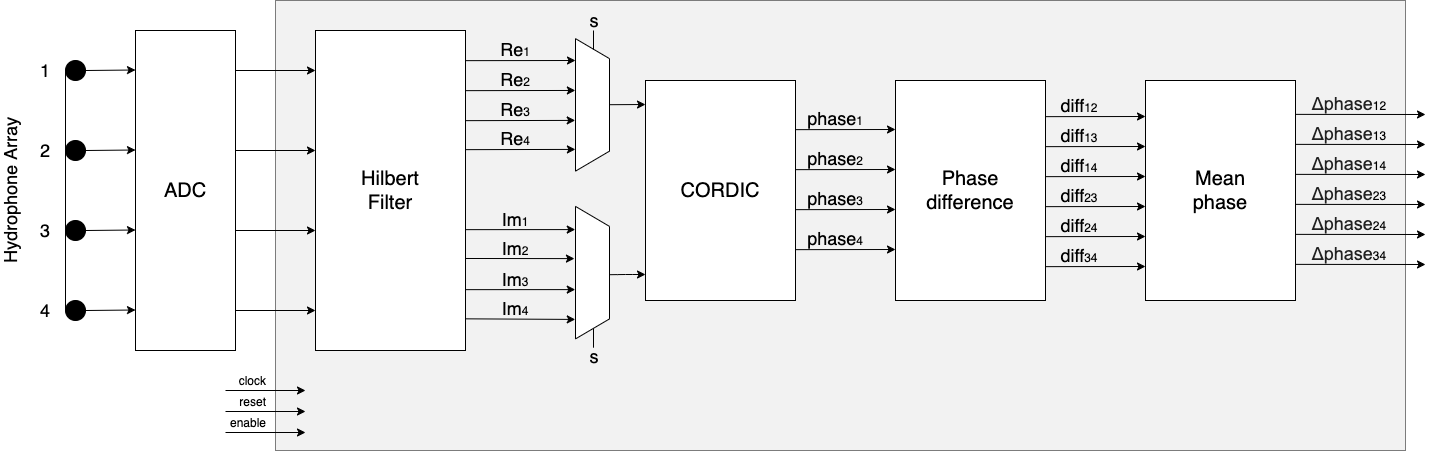
\includegraphics[width=1\textwidth]{figures/hdl-diagram-all}}
	\captionsetup{justification=centering,margin=2cm}
	\caption{Top level architecture}
	\label{fig:module-all}
\end{figure}

The sampling frequency of the input signals is 244 kHz and the whole digital circuit works with a global clock signal equal to 125 MHz. Thus, there are 512 clock cycles available between each two arriving signal samples and, as the calculations to perform are simple, these are more than enough to originate the outputs, therefore this architecture does not involve time constraints. Instead, it focuses on minimizing the used area since it is part of a complex system that already uses a substantial part of the FPGA resources.

In order to describe the efforts to minimize the used area, all module sub components are detailed next, namely the Hilbert filter, CORDIC, Phase difference and Mean phase.

\subsubsection{Hilbert Filter}

The signals coming from the ADC are purely real so they need to be converted to their analytic representation. This is achieved by using a module based on a Hilbert FIR filter, which derives the complex representation by comprehending the original real signal and its Hilbert transform. 

The Hilbert transform definition is given by (\ref{eq:hilbert_integral}) \cite{hilbert-def}, where $x(t)$ is the original signal and $P$ is the Cauchy principal value.

\begin{eqnarray}
	H(x)(t) = \frac{1}{\pi} \ P \int_{-\infty}^{\infty}\frac{x(\tau)}{t-\tau}d\tau
	\label{eq:hilbert_integral}
\end{eqnarray}

An 8-th order Hilbert FIR filter was designed using the Matlab function \textit{designfilt} and has only 4 non-zero coefficients. Although this will provide an inaccurate calculation for the instantaneous phase of the input signals along the signal period, it has been observed with Matlab simulations that this approximation will be enough for obtain an averaged phase difference within a few degrees. Nevertheless, the length of the Hilbert filter can be easily increased without a significant impact in the digital design complexity.

The 8th order Hilbert filters coefficients $a_k, k=1,...,7$ respect an odd anti-symmetry, i.e. $a_{1} = - a_{7}$ and $a_{3} = - a_{5}$. Thus, the imaginary and real components of the input signal $x_i$ are obtained by following equations (\ref{eq:hilbert_imeq}) and (\ref{eq:hilbert_reeq}). 

\begin{eqnarray}
	&Imag_0 = a_{1} \ x_{-1} +a_{3} \ x_{-3} + a_{5} \ x_{-5} + a_{7} \ x_{-7} \\
	\label{eq:hilbert_imeq}
	&Real_0 = x_{-4} 
	\label{eq:hilbert_reeq}
\end{eqnarray}

In order to implement this filter, the most common approach is to use a chain of registers that integrate multiple adders and multipliers, so that the calculations take less clock cycles to obtain a valid result, similarly to the work in \cite{hilbert-fpga}. However, since the goal of this implementation is to minimize area, then an alternative approach was formulated which uses only one multiplier and one adder. As can be observed in the filter equation, all odd samples need to be multiplied by a coefficient and summed with each other. Therefore, by using a circular shifting register chain \ref{fig:hilbert-chai} for each arriving signal, it is possible to position each of the buffer chain's samples in register $x_8$, which is used for external calculations.

\begin{figure}[!htbp]
	\makebox[\textwidth][c]{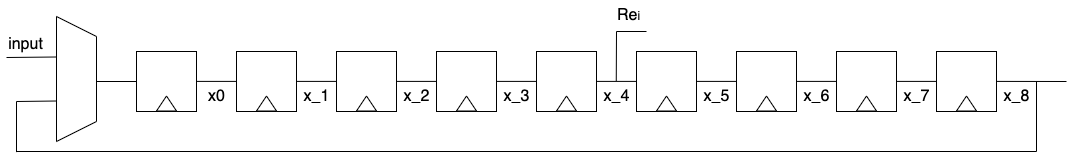
\includegraphics[width=0.9\textwidth]{figures/hilbert-filt-chain}}
	\captionsetup{justification=centering,margin=2cm}
	\caption{Hilbert Filter circular shifting register chain}
	\label{fig:hilbert-chai}
\end{figure}

In a more comprehensive view, the register chains $HF_{Ci}$ are integrated with the remaining block elements as represented in \ref{fig:hilbert-all}. The four shift-register chains receive four signals as input and output the real and imaginary components, $Real_i$ and $Imag_i$, for each of them.

\begin{figure}[!htbp]
	\makebox[\textwidth][c]{\includegraphics[width=0.9\textwidth]{figures/hilbert-filt-all}}
	\captionsetup{justification=centering,margin=2cm}
	\caption{Hilbert Filter block diagram}
	\label{fig:hilbert-all}
\end{figure}

The implementation contains a series of design decisions that lead to decreased area occupation, presented as follows :

\begin{itemize}
	\item The four register chains are multiplexed so that the module needs only one multiplier and one adder to calculate the Hilbert transform for all signals;
	
	\item Since the coefficients have odd symmetric pairs, then only two variables and their symmetric value are needed, which will be referred as $c_a = a_7 = - a_1$ and $c_b = a_5 = - a_3$. For even samples, associated with coefficients equal to zero, a controller unit is responsible for skipping the multiplication, which saves energy. For odd samples, the control unit alternates between the positive and negative coefficients to be multiplied. The control unit settings are summarized in table \ref{tab:coeffs-control-unit} for each register chain sample. 
	
	\begin{table}[!htbp] %use H to adjust
		\begin{center}
			\makebox[\textwidth]{
				\begin{tabular}{ c | c  c  }
					%\hline
					\toprule
					\multicolumn{1}{c|}{} & Multiplier Coefficient  & Adder mode\\	
					\midrule
					\multicolumn{1}{c|}{$a_0$} &  0 & -\\
					\midrule
					\multicolumn{1}{c|}{$a_1$} &  -$c_a$ & -\\
					\midrule
					\multicolumn{1}{c|}{$a_2$} &  0 & -\\
					\midrule
					\multicolumn{1}{c|}{$a_3$} &  -$c_b$ & -\\
					\midrule
					\multicolumn{1}{c|}{$a_4$} & 0 & +\\
					\midrule
					\multicolumn{1}{c|}{$a_5$} &  $c_b$ & +\\
					\midrule
					\multicolumn{1}{c|}{$a_6$} & 0 &+ \\
					\midrule
					\multicolumn{1}{c|}{$a_7$} &  $c_a$ & +\\
					\midrule
					\multicolumn{1}{c|}{$a_8$} & 0 &+ \\
					\bottomrule 
			\end{tabular}}
			\caption{Hilbert filter control unit settings for each processed sample with $c_a = 0.23932$ and $c_b = 0.62610$}
			\label{tab:coeffs-control-unit}
		\end{center}
	\end{table}
	
	\item The negative coefficients are achieved by subtracting the result of $a_{i} \ x_{-i}$, i.e. negating the adder, so only one adder block is necessary;
	
	\item A register is placed after the adder so that it interactively accumulates the value that is correspondent to the imaginary component $Im_i$ after the full chain circle shifting.
	
\end{itemize}

Having cleared the implementation details, it is possible to deduce that each $HF_{Ci}$ takes 9 clock cycles to be processed. Therefore, the entire calculation of the complex representation of the four input signals takes $9 \times 4$ clock cycles plus one additional cycle to update the outputs.

\subsubsection{CORDIC}

The CORDIC algorithm is used for real-time trigonometric and exponential calculations, as well as polar to rectangular conversions and vice-versa, using iterative vector rotations. 

The implemented CORDIC module has a sequential structure, as it occupies the least area, and it is responsible for receiving the real and imaginary components of a signal and calculating its phase. There are two possible modes of operation from which it is used the vectoring mode (VM), whose algorithm computes the magnitude and phase of the input vector $(x_0, y_0)$ from the x-axis \cite{cordic-def}. This is achieved by iteratively approximating the phase through angle microrotations of $\alpha_i = \ \pm atan(2^{-i})$ which are summed originating an approximated phase. The result is given in a 16 bit value, which is composed by 9 bits for the integer part and 7 bits that represent the fractional portion. 

The CORDIC iterations are expressed by (\ref{eq:cordic-iter-x}), (\ref{eq:cordic-iter-y}) and (\ref{eq:cordic-iter-z}) for $d_i$ belonging to \{-1,1\}.

\begin{eqnarray}
	& x_{i+1} = x_i - d_i \ 2^{-1} \ y_i
	\label{eq:cordic-iter-x}  \\
	& y_{i+1} = y_i + d_i \ 2^{-1} \ x_i
	\label{eq:cordic-iter-y} \\
	& z_{i+1} = z_i - d_i \ \alpha_i
	\label{eq:cordic-iter-z}
\end{eqnarray}

The CORDIC logic uses a 16 element ROM (Read-Only Memory) that stores the $atan(2^{-1})$ values required for the algorithm. Additionally, another sub component provides a binary counter that defines the number of performed iterations and it is also responsible for generating the address to access the ROM. 

Considering that the CORDIC module uses 16 clock cycles to run through the entire ROM and one additional cycle to update the outputs. Therefore, the design uses only one CORDIC module with multiplexed inputs so the process takes $17 \times 4$ plus one, to update the global outputs, in a total of 69 clock cycles.

\subsubsection{Phase Difference}

This sub module is responsible for computing the phase differences between the previously determined signals' phases, $phase_i$. For four inputs $phase_i$, it is generated the difference between all pairs of different hydrophones, $h_ih_j$: $h_1h_2$, $h_1h_3$, $h_1h_4$, $h_2h_3$, $h_2h_4$ and $h_3h_4$.

This is achieved using a single subtractor which has multiplexed inputs so that the calculations can be executed within the 512 clock cycles with only one block of hardware, instead of dedicated subtractor for each calculation. 

The result is given in a 16 bit value, which is composed by 10 bits for the integer part and 6 bits that represent the fractional portion. 

\subsubsection{Mean Phase}

Finally, the last module implements a moving window averaging filter, with a window size $N = 2^k$ configured by the parameter k, with values from 1 to 6. The final averaged phase differences are in the range [-180º,+180º], represented in 16 bits with 7 bits for the fractional part.

\subsection{Implementation Results}

The design was synthesized to a XILINX XC7Z010 Zynq \cite{xilinx-board} device and integrated in the digital signal processing system implemented in a Red Pitaya platform. Although this block is only a part of a more complex signal processing system that also includes the correlation calculators as described in \cite{afonso-thesis}, it occupies only 1216 flip-flops and 1462 Look-up tables, which represents a small fraction of the available FPGA resources. Besides, the sequential implementation of the Hilbert FIR filter and CORDIC module and the sharing of the modules among the four input signals has reduced the size of a previous preliminary implementation which used more than 10k flip-flops and 6k Loop-up tables.


%----------------------------------------------------------------------------------
\section{Doppler Effect}

The implemented process uses the information of the transmitted signal's operating frequency in order to compute the phase differences and determine the overall times of arrival. However, in real scenarios the environmental and the operational conditions will distort the frequency perceived by the receiver due to the relative movement between the acoustic source and the receiver.

In order to evaluate if the Doppler effect influences the system, it is possible to calculate the frequency deviation observed for a known relative speed between vehicles. Considering that the relative speed between the transmitter and the receiver is denoted as $relative\_speed$ and using a fixed sound speed, $c_s$, with a determined frequency of the transmitted signal, the relation (\ref{eq:doppler}) \cite{doppler-eq} can be established. 

\begin{eqnarray}
	&freq\_deviation = \frac{relative\_speed}{c_s} \times signal\_freq
	\label{eq:doppler}
\end{eqnarray}

Therefore, considering a maximum relative velocity between the transmitter and the receiver equal to $\pm \ 5 m/s$, this will impact in a frequency deviation perceived by the receiver equal to $\pm \ 81Hz$, which corresponds to a relative error of 0.33\% of the nominal frequency and approximately the same relative deviation for the period of the signal reaching the receiver. As the time differences calculated from the phase differences are directly proportional to the expected signal period, concerning the calculation of the time difference of arrival to different hidrophones, the Doppler effect has been considered negligible.

A way to prevent this deviation is to integrate a frequency detector which senses the relative navigation speed in real time and adapts the used frequency. This mechanism is not integrated in the present research work.
\chapter{Research Problem} \label{chap:problem}

This chapter intends to clarify the problem addressed by the present dissertation. 

\section{Problem Statement} \label{sec:prob-state}

As previously mentioned in chapter \ref{chap:intro}, it is considered a scenario where an AUV is taking part on a long-term underwater mission. When it is in course, the moving survey AUV periodically sends known signals to the surface with a pinger, so it can be identified. The mule AUV, which is provided with a three dimensional array of hydrophones, receives the signal and estimates the position of the other AUV to navigate near it. The described communication system is illustrated in figure \ref{fig:auv_scene}. 

\note{redefinir}

\begin{figure}[!htbp]
	\centering
	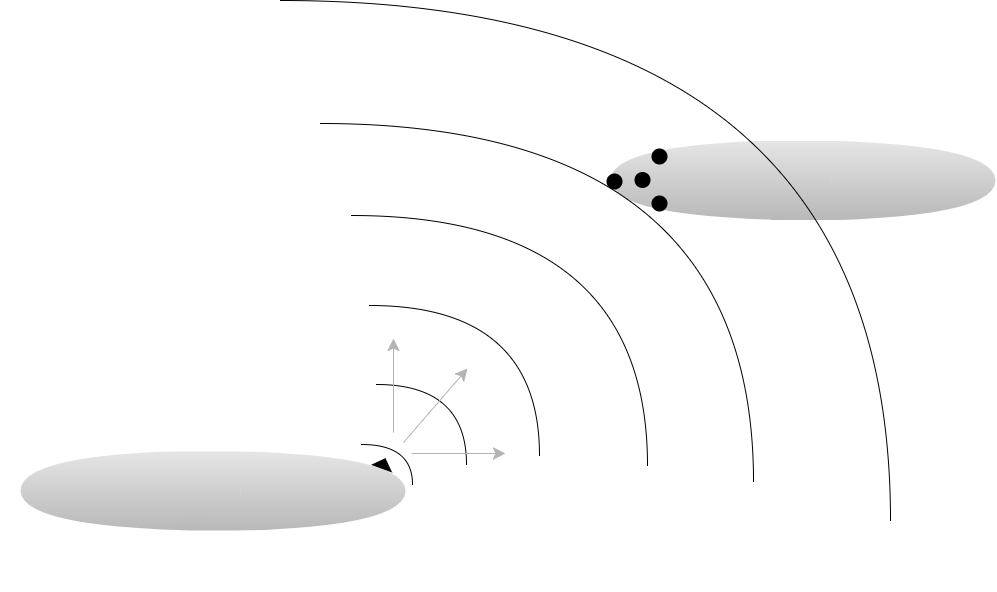
\includegraphics[width=0.7\textwidth]{figures/proposed-solution}
	\caption{Communication System}
	\label{fig:auv_scene}
\end{figure}

This partial system was developed in previous dissertations and research work, which can be better understood in \cite{afonso-thesis}. Briefly, the system consists on a transducer of four hydrophones forming a 3D array deployed on the mule AUV. This array will receive the same signal wave front. The system then calculates the cross-correlation between the received and expected signals, which is a BPSK modulated binary sequence. The cross-correlation peak indicates the distance between AUVs and it is calculated with timing resolution corresponding to 1 sampling period of the acquired signal, which in the developed systems corresponds approximately to 6mm (with a sampling frequency of 244kHz).

Since we are referring to an USBL system and due to the limitations in dimension of the AUV that will integrate this system, the hydrophones have to be placed within a few centimeters from each other. For this reason, the obtained time resolution by using only the cross-correlation, corresponding to a maximum distance accuracy of approximately 6mm, will not be enough for the calculation of the angle of arrival of the sound wave. Thus, in this thesis it is intended to refine this measurement by additionally calculating the phase differences of the arriving signals to each hydrophone. 

Upon having this measurement refined, the information of the phase difference between hydrophones, as well as additional data from modules already implemented, will serve as base to develop a software mechanism that estimates the angle of arrival of the received signal to the hydrophone array.

Finally, as an effort to improve the underwater localization system, a set of tests have to be performed in order to evaluate the robustness and estimation accuracy of the developed system. This study intends to prove the hypothesis declared in \ref{sec:hypoth-rq} and consequently respond to some of the defined research questions.


\section{Hypothesis and Research Questions} \label{sec:hypoth-rq}

This dissertation intends to complement previous research work by adding the design of an integral hardware model and respond to a core research hypothesis which serves as fundamental investigation purpose.

The first part of the developed work focuses on the practical implementation of a HDL model which has as premise the following idea: \textit{"Implementing a system that utilizes the phase differences between the arriving signals to an array of hydrophones, increases the accuracy of the time of arrival determination of the current system, which consequently improves the angle of arrival estimation."}

The second part of the research work focuses on the study and experimentation with methods that improve the localization accuracy for underwater applications. This research hypothesis can be stated as:
\\

\textit{"Using a real-time dynamic reconfigurable hydrophone array improves the underwater localization accuracy"}
\\

Attending the proposed hypothesis, the topics that are intended to be explored and discussed in this thesis's work can be summarized in the following research questions:

%Research Questions
\begin{itemize}

	\item \textbf{RQ1: }\textit{How should a system be implemented so it is capable of calculating phase differences between arriving signals at four different hydrophones and, simultaneously, be compatible with the available space in the FPGA?}
	
	\item \textbf{RQ2: }\textit{What method should be adopted in order to efficiently estimate the angle of arrival of a signal to an array of four hydrophones?}
	
	\item \textbf{RQ3: }\textit{What metrics should be used to evaluate which hydrophone configuration is optimal for a certain angle of arrival?}
	
	\item \textbf{RQ4: }\textit{How should the system be developed in order to improve the vision angle of the hydrophone array?}
	
\end{itemize}

These questions summarize the main topic points which are explored in the scope of this thesis and are the essential inquiries that it intends to answer.


\section{Validation Methods} \label{sec:validation}

The validation of scientific work is a key factor to demonstrate how reliable and effective it is. In this thesis, three essential methods are used to validate the functionality of the developed techniques:

\begin{itemize}
	
	\item \textbf{Simulation}
	
	The considered immediate approach to evaluate the functionality and behavior of the system consists in creating a set of simulation procedures which are as close as possible to the real environment and the physical system. These simulations were made as MATLAB scripts carefully designed to integrate realistic parameters, such as expected environment noise and other limitations.
	
	\item \textbf{Scientifically recognized methods}
	
	When composing a system, it can be useful comparing the studied approach with widely used methods which are recognized in the scientific community as robust and trustworthy. By doing this, we can gain a level of confidence in the developed system and in the obtained results.
	
	\item \textbf{Field experiments}
	
	After having the analytical methods and simulations coherent, it is essential then to test the system in a real environment in order to understand if the system still works correctly when real conditions are added. By testing it in a real application it is possible to take conclusions about its robustness and consider improvements or refinements for the system.
	
\end{itemize}

\chapter{Ultra-Short Baseline System} \label{chap:proposed_sys}

This chapter is dedicated to the presentation and overall explanation of the developed system, highlighting its capabilities, the used methodologies and overall design strategies. 
The system will be presented in two distinct sections. The first component is the HDL module, which falls into the spectrum of hardware design and requires insight on hardware development and good practices. The second section relies on software development to complement the functionality of the mentioned module, so that is possible to deliver the desired result.

\section{HDL Module Architecture} \label{subchap:HDL module}

The system which is proposed to be implemented in this research work has as input 4 signals which are received by each hydrophone of the array, and outputs an average phase difference between all combinations of pairs of hydrophones. 

\note{
- regras basicas de hardware development\\
- sistema sincrono, available clock cycles globais\\
- hardware limitations\\
- tamanho das entradas
arg}


\begin{enumerate}
	\item Hilbert Filter
	\item Cordic
	\item phasediff
	\item phasemean
\end{enumerate}

\subsection{Module components}

apresentar esquema global menos pormenorizado

\subsubsection{Hilbert Filter}

\begin{eqnarray}
H(f)(t) = \frac{1}{\pi}\int_{-\infty}^{\infty}\frac{f(\tau)}{t-\tau}d\tau
\label{eq:hilbert_integral}
\end{eqnarray}

\begin{eqnarray}
&Imag_0 = x_{-1}*c_1 + x_{-3}*c_3 + x_{-5}*c_5 + x_{-7}*c_7
\label{eq:hilbert_imeq}
\end{eqnarray}

\begin{eqnarray}
&Real_0 = x_{-4} 
\label{eq:hilbert_reeq}
\end{eqnarray}

\note{
- matematica brevemente, equação base, resposta impulsional, ganho, coeficientes e ordem usada \\
- schematics  \\
- explicar design decisions \\
- descrever brevemente flow do sinal no hardware
}

\subsubsection{Cordic}
\note{
- descriçao do que faz \\
- entradas e saídas, clocks, ROM
}

\subsubsection{phasediff}
\note{
-pequeno esquema \\
- 1 sub
}

\subsubsection{phasemean}
- pequeno esquema \\
- N accumulated \\

\subsection{Analysis}

\note{present used resources\\ overall achievement}


\section{Position Estimator} \label{subsec:AoA}

The proposed position estimator uses vector algebra, the phase differences obtained from the system described in \ref{subchap:HDL module}, synchronization elements and additional mechanisms that will be further explained in the present section.

\subsection{Preliminary considerations}

In order to better understand the mechanisms used in the development of the estimator, some preliminary considerations are laid out. These contemplate the following topics: the number of used sensors for the estimation; a phase ambiguity issue that affects the ToA determination; the relation between the phase differences of hydrophones in known relative positions and the possible location of the transmitter; an approximation used in the ToA measurement; the influence of the Doppler effect.

\subsubsection{Number of sensors}
For the estimation of the position in 3D space, a multilateration approach was used. As explained in \ref{subsec:multilateration}, the concept of multilateration combines the information of the relative distances between multiple sensors and a target in order to locate it. 

In the present case, a total of four sensors are needed so that it is possible to define the position of target. Using only two sensors, two possibility spheres are formed around these sensors whose intersection originates a circle that contains the location possible solutions. By adding a third sensor, this circle is intersected by another sphere which originates only two location possibilities. Finally, a fourth sensor is added so that it is possible to exactly differentiate which one of the two final solutions is the accurate location solution. 

\subsubsection{Phase Ambiguity}

When the information about the time of arrival of a signal is available, it is relatively easy to estimate the range of the communication since there can be a direct conversion between them. However, when dealing with phase differences, there is no exact time notion, so it is necessary to start by defining a reference point. 

Considering sinusoidal signals, when we have an array with four hydrophones spatially placed to form a 3D layout, the signal that is arriving to each  hydrophone in different times consequently have different phases. However, since sinusoidal signals are periodic, this means that for different signal periods the same phase value is observed, i.e. the phase is ambiguous. It is possible to observe this phenomenon in figure \ref{fig:phasediff}. In this illustration, $\alpha$ represents the observable phase difference of hydrophone $H_4$ to the reference point $H_1$. However, the actual phase difference which is intended to obtain, $\Delta p_4$, is one period of the signal, $\lambda$, added to the observable phase $\alpha$.

\begin{figure}[!htbp]
	\centering
	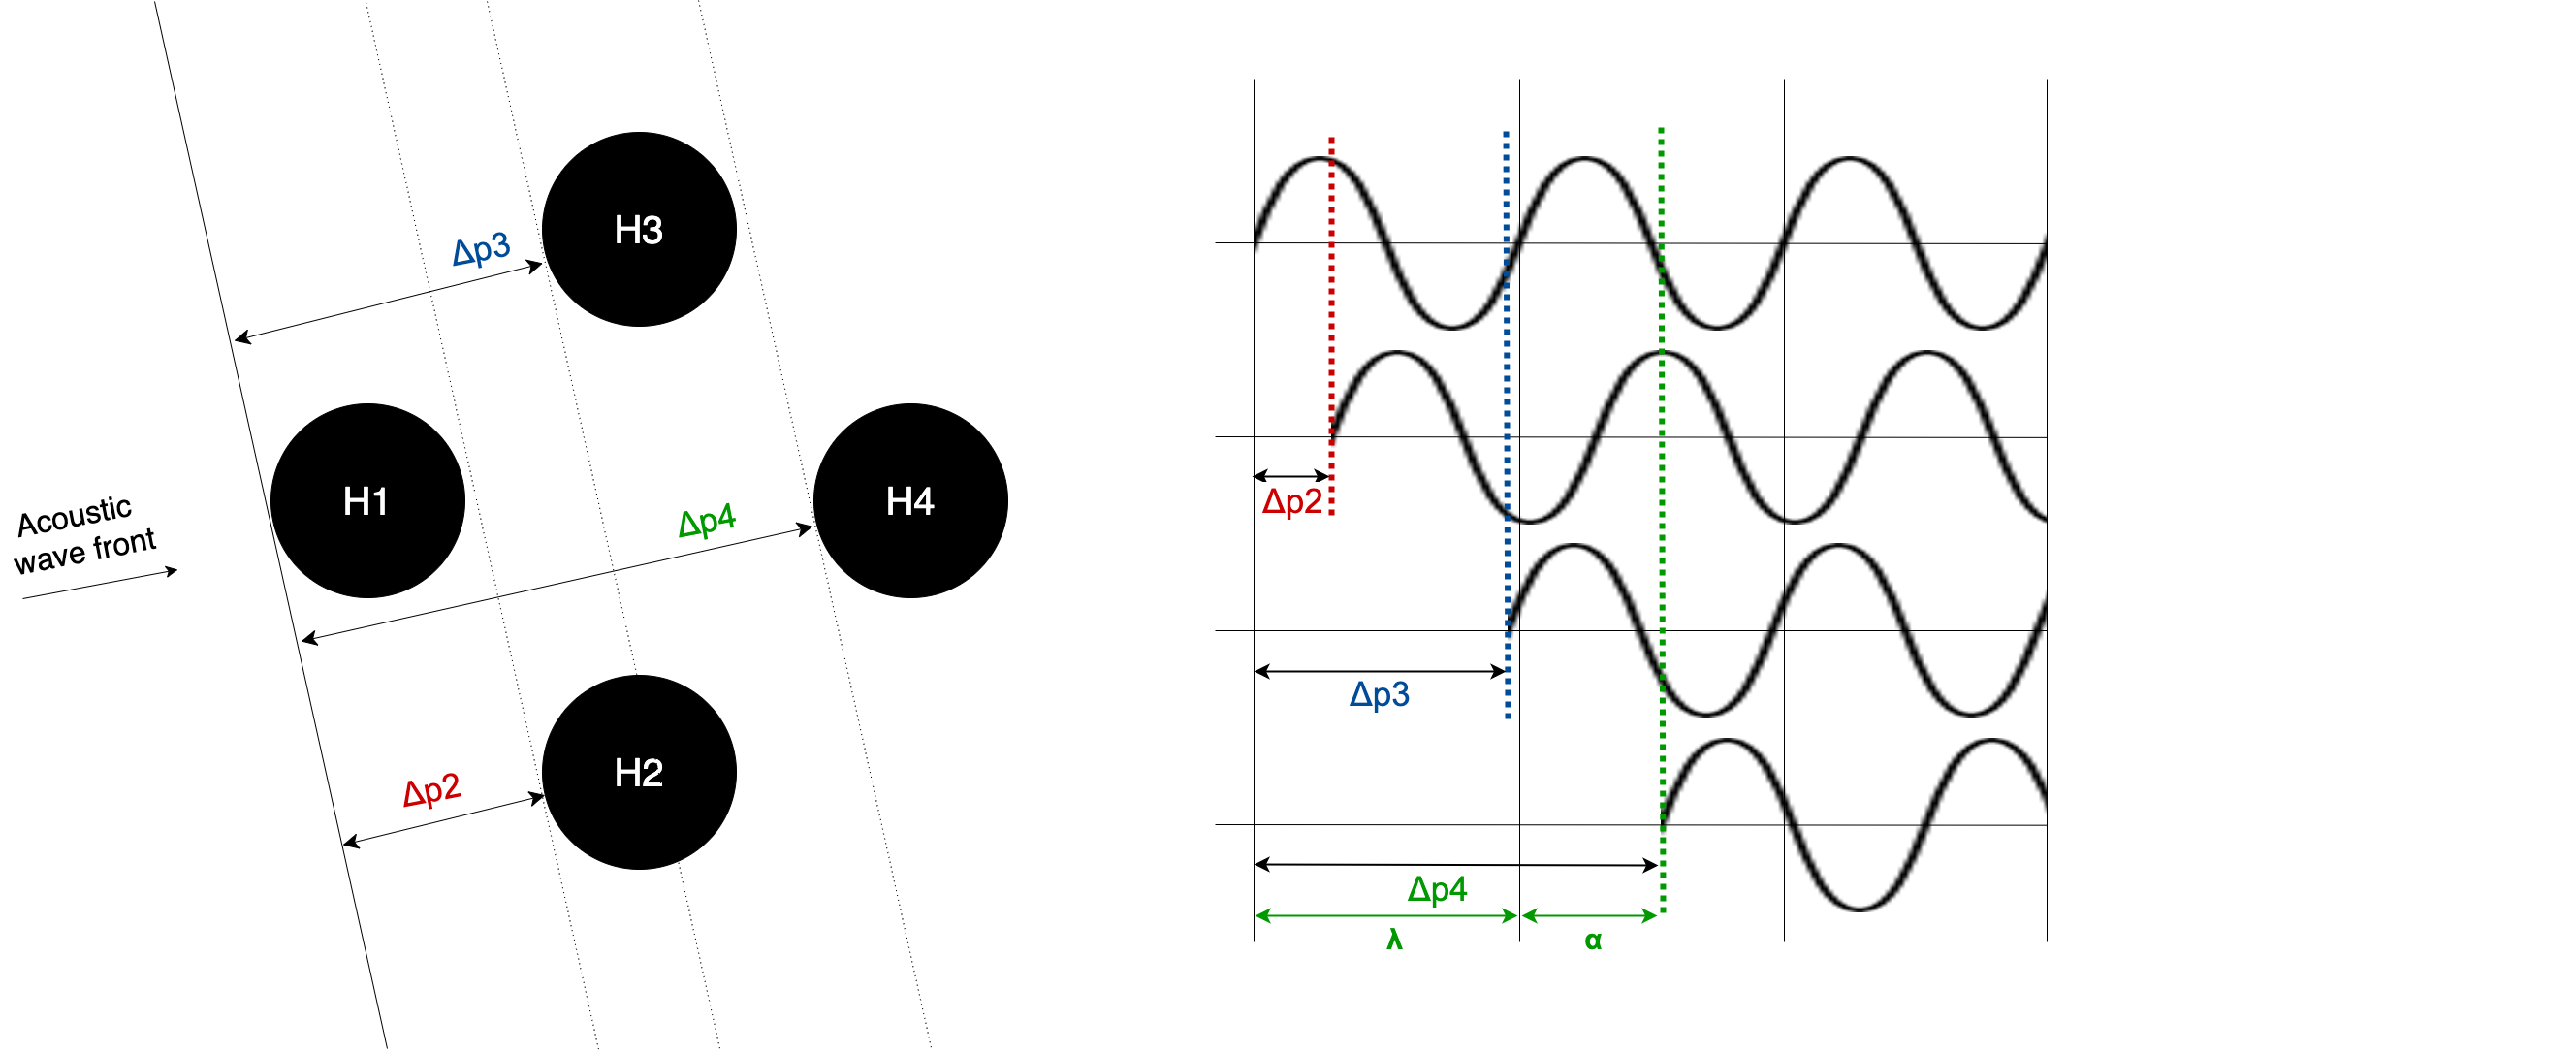
\includegraphics[width=1.2\textwidth]{figures/phase-diff}
	\caption{Phase difference to reference point and phase ambiguity}
	\label{fig:phasediff}
\end{figure}

For this reason, it is crucial to consider that the phase difference is given by the obtained phase value added by the number of periods ahead from the considered reference period.

In the system under study, the sent signals work with a operation frequency of 24.4 $kHz$. The corresponding signal period is $T = \frac{1}{24400} $ seconds which, considering the underwater acoustic speed \textit{c} equal to a standard 1500 $m/s$, the wavelength is approximately equal to $\lambda = \frac{T}{c} = 6.1 cm$. Having this into consideration, after obtaining the time of arrival to each hydrophone given by the cross correlation instances, besides the reference one, it is possible to conclude if the phase shift is superior to one period by analyzing if the time difference is greater than the duration of one period \textit{T}. In figure \ref{fig:phasediff}, each mentioned time difference between $H_1$ and $H_2$, $H_3$ and $H_4$ is converted to the corresponding phase differences $\Delta p_2$, $\Delta p_3$ and $\Delta p_4$.

%From this phase differences, it is possible to estimate the angle of arrival from which the acoustic wave is coming from by comparing all pairs of hydrophones: H1-H2, H1-H3, H1-H4, H2-H3, H2-H4, H3-H4. 

One possibility to solve phase ambiguity in this system would be to place the four hydrophones with a baseline spacing inferior to $\frac{1}{2}$ of a wavelength, since the maximum reached by phase difference is 180 degrees. This way it would be possible to immediately deduce the phase difference since it would always be contained in one period. However, positioning the hydrophones closer together leads to smaller  values,causing a consequent increase on the estimation error due to varying environment conditions (briefly enumerated in \ref{subsec: acoustic-channel}). Additionally, since the hydrophones to be used in this system have a corresponding diameter of roughly half of a wavelength, they would not allow to execute the mentioned configuration and so this possibility will not be contemplated.

In order to compensate this phase ambiguity, a simple relation was developed which allows to calculate the absolute time difference between the moment a signal is received by hydrophone A, $T_A$, and when the same signal is received by a further hydrophone B, $T_B$. Figure \ref{fig:ambiguity} illustrates this association, where the represented sinusoidal waves correspond to the same signal arriving at hydrophones A and B. This correspondence uses the time stamps obtained by the correlation peaks combined with the calculated phase difference, that is determined in parallel, so that the measurement is more accurate. Equation \ref{eq:phase-amb} translates this relation, where $t_1$ and $t_2$ are the correlation peaks obtained from the signal arriving at hydrophone A and B, respectively, and so by rounding for the next integer number the difference between the correlation peaks, $t_2 - t_1$, we will obtain in which period, $T$, of signal in A will the signal in B arrive. Then the measurement is improved by subtracting a phase difference, $\theta_B - \theta_A$, so that the instant in which the signal is detected in hydrophone B can be defined. 

\begin{figure}[!htbp]
	\centering
	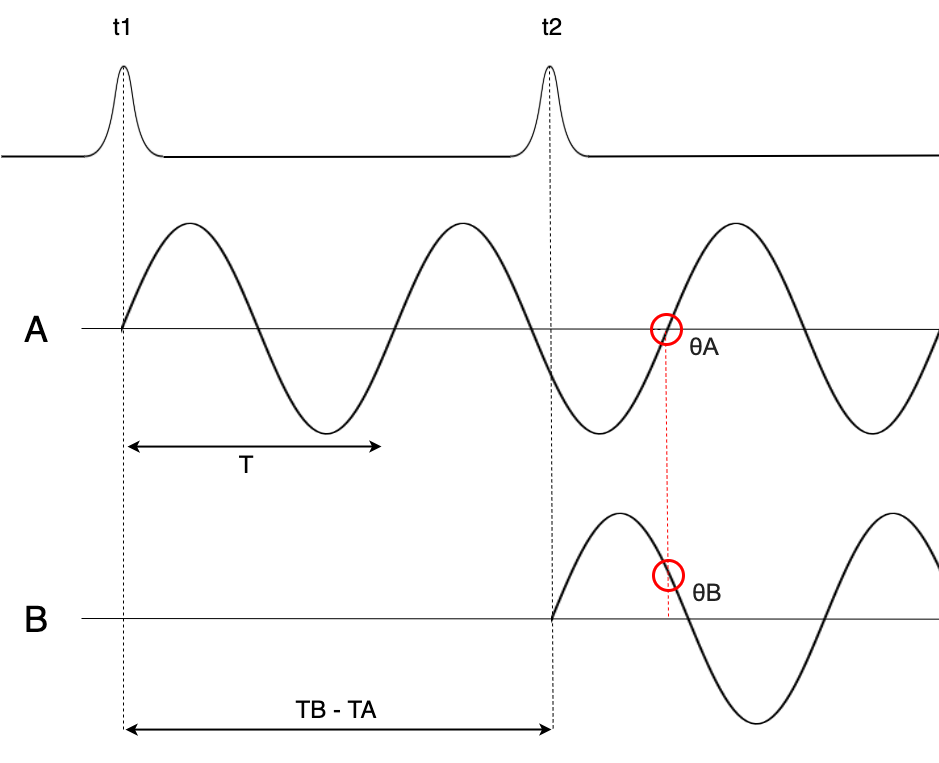
\includegraphics[width=0.6\textwidth]{figures/ambiguity}
	\captionsetup{justification=centering,margin=2cm}
	\caption{Ambiguity correction through correlation and phase difference}
	\label{fig:ambiguity}
\end{figure}

\begin{eqnarray}
& T_B - T_A = round(\frac{t_2-t_1}{T}) - (\theta_B - \theta_A)
\label{eq:phase-amb}
\end{eqnarray}

\subsubsection{Hydrophone position in relation to ToA}
To better understand the location estimation of an acoustic source in relation to the position of a pair of hydrophones, we can initially adopt the two dimensional scenario of figure \ref{fig:hyper}. 

Considering two hydrophones at known relative positions $(-f,0)$ and $(f,0)$, we can model all possible acoustic source locations for a specific ToA through hyperbolas. This is due to the fact that, by definition, the sum of the distances from the focus of each hyperbole, where each hydrophone is placed, to any point of the hyperbolic geometry corresponds to a constant value. 
This means that, in figure \ref{fig:hyper}, any point $(x,y)$ that is contained in the hyperbole corresponds to a constant $|d_2-d_1|$ value which, after some formulation, is in fact equal to $2*v$ or the distance between the vertexes of each hydrophone's hyperbola. Therefore, it is possible to trace a hyperbole that represents the positions of the target in space both based on their distance and the signal's ToA. In the exceptional case where $d_3=d_4$, we can observe that the possible positions are represented by an equidistant straight line to each hydrophone, such as the y axis.

\begin{figure}[!htbp]
	\centering
	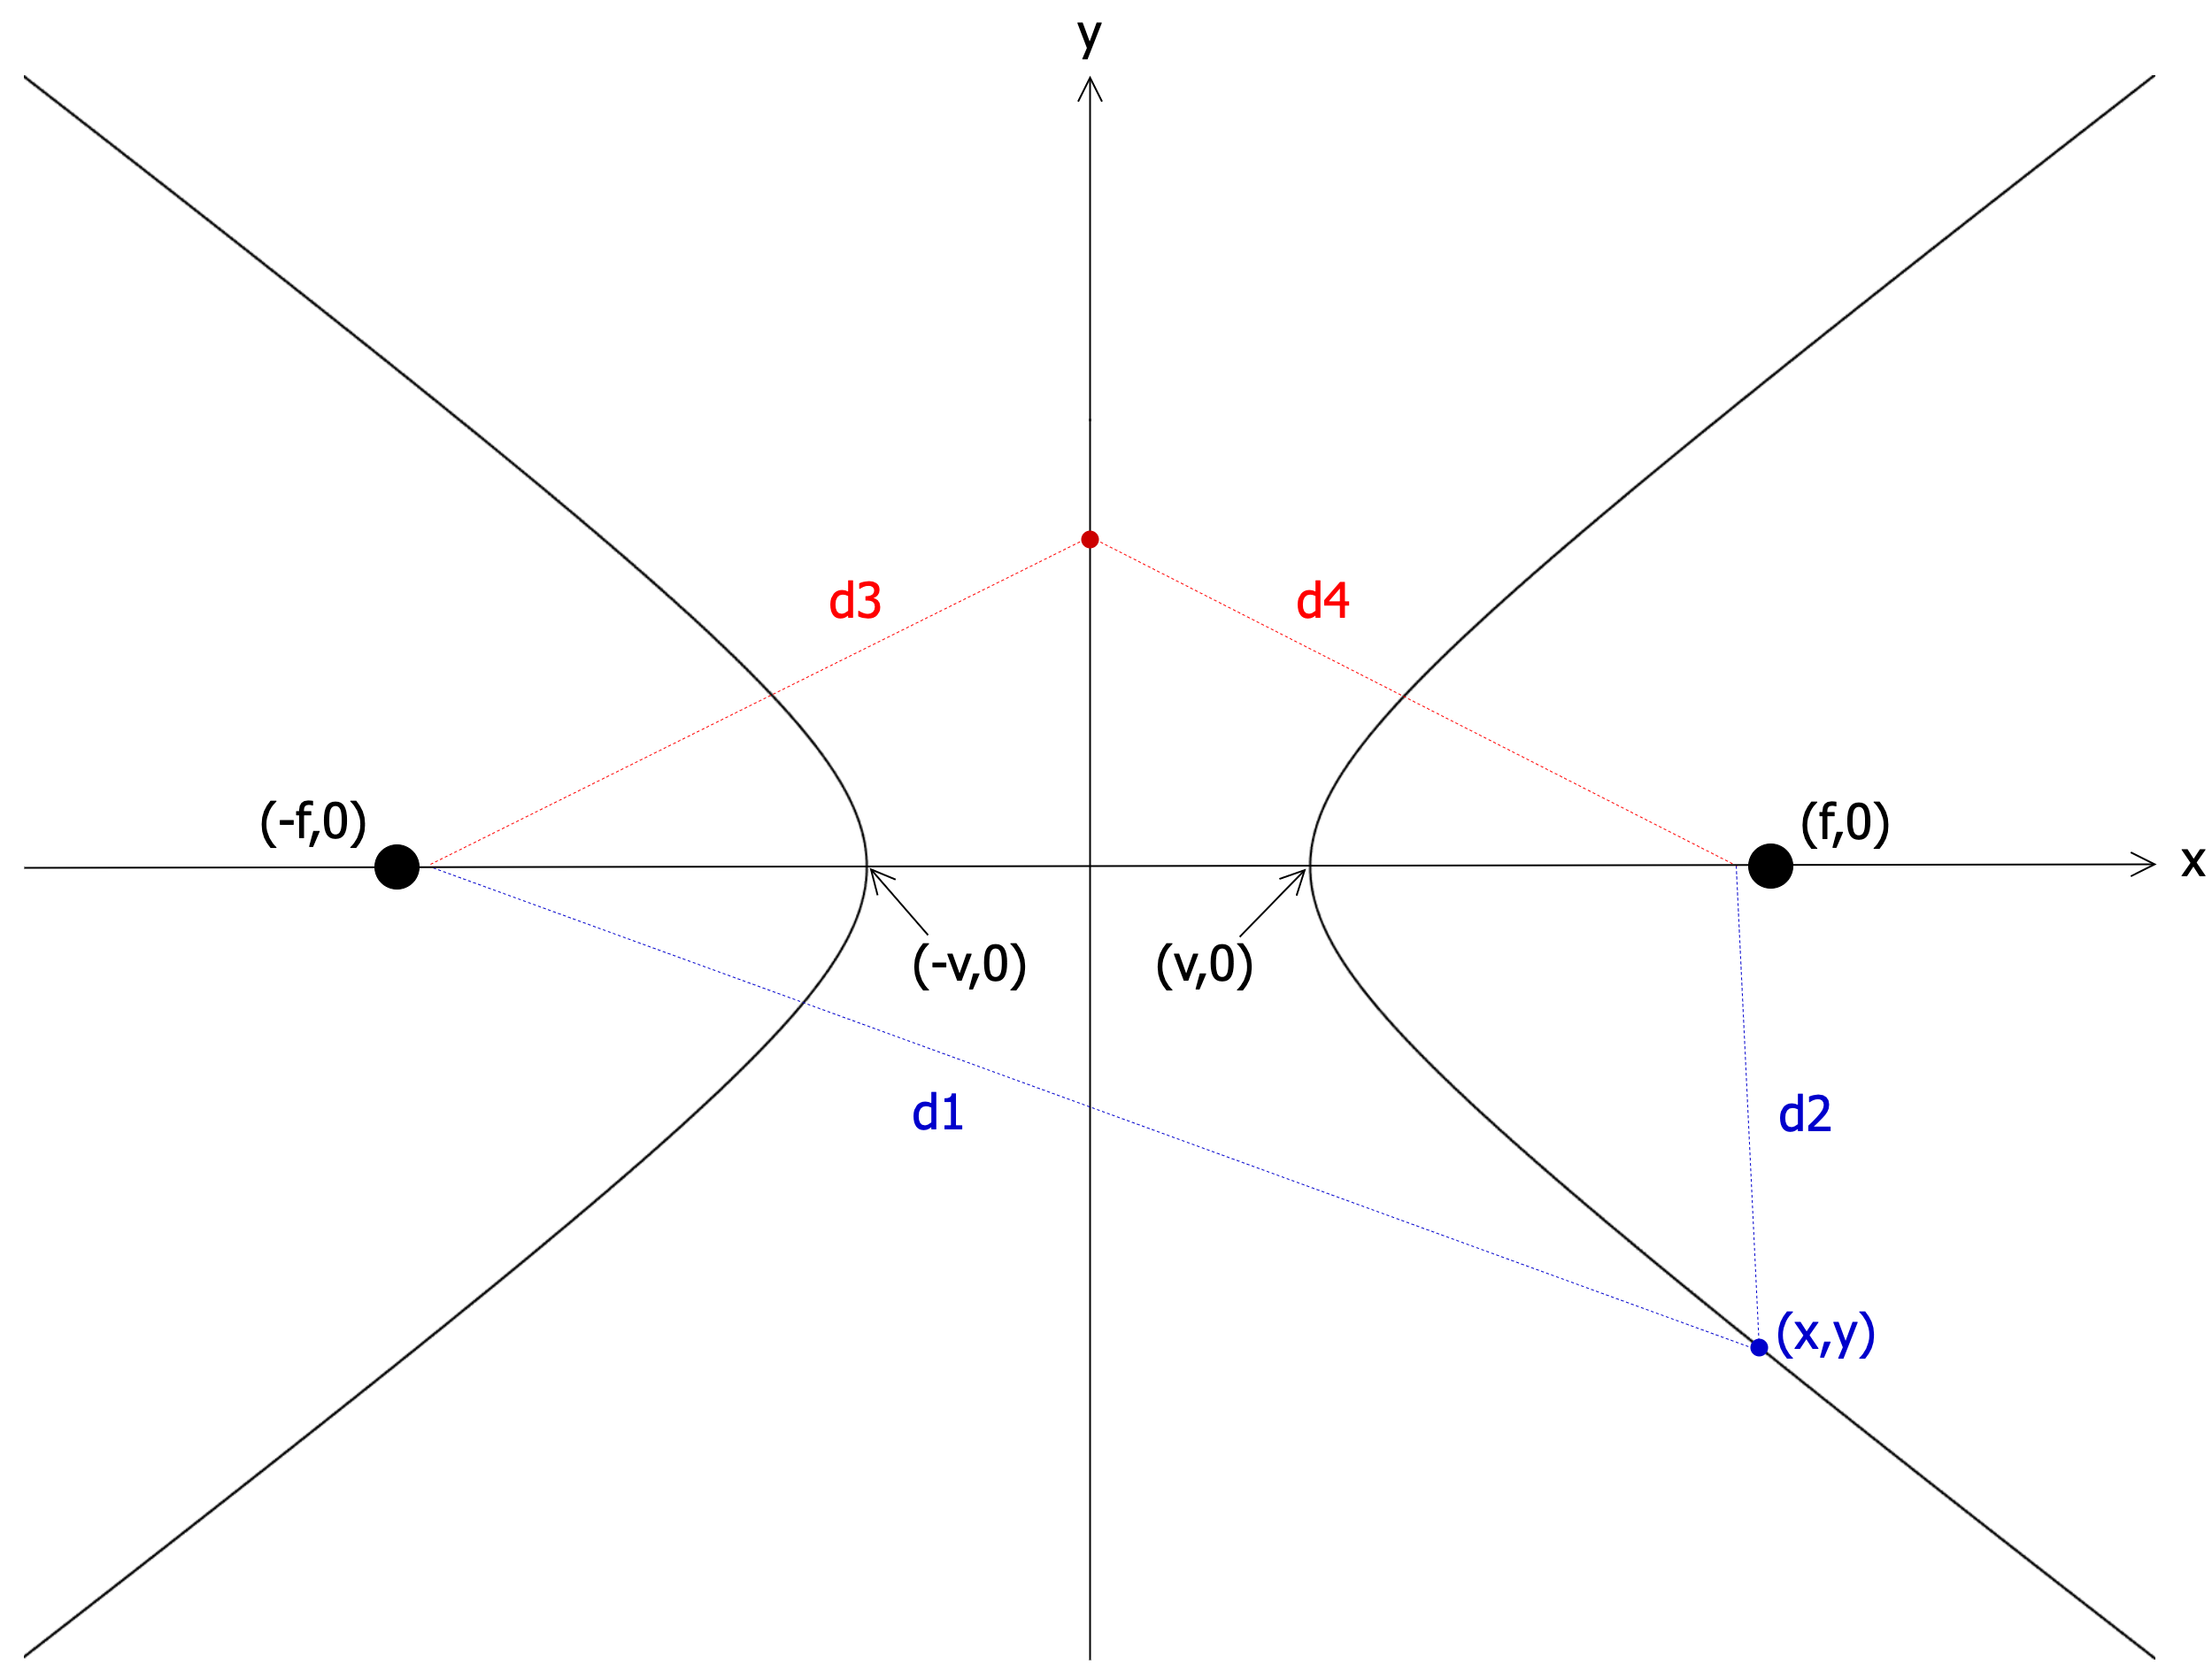
\includegraphics[width=0.8\textwidth]{figures/hyperbole-dist}
	\captionsetup{justification=centering,margin=2cm}
	\caption{Hyperbolic representation of acoustic source position possibilities in relation to ToA to two hydrophones}
	\label{fig:hyper}
\end{figure}

\subsubsection{ToA approximation} \label{subsubsec:toa-approx}

In order to estimate the location of an acoustic source we take into account the phase differences between each pair of hydrophones, carefully explained in section \ref{subchap:HDL module}. These phase differences can be translated into periods of the signal which combined with the ToA obtained from correlation of arriving acoustic signals are equivalent to relative distances.

Following the previous idea, it is possible to model the distance of one sensor to the target based on the known distance of a second sensor to the same target. 
This is to say that for two sensors with known relative positions where hydrophone 1 is the closer to the target, the distance from hydrophone i to the target, $D_i$, can be expressed as the distance of hydrophone j to the target, $D_j$, added by the time difference of arrival, $\Delta t_{ij}$, multiplied by the propagation velocity, $c_s$. Overall, this relationship is declared in equation \ref{eq:dist_to_target}.

\begin{eqnarray}
& D_i = D_j + \Delta t_{ij} * c_s
\label{eq:dist_to_target}
\end{eqnarray}

Therefore, the same logic can be applied for multiple hydrophones. In the present work, in which it is considered a system with four hydrophones, a synchronization mechanism allows to determine the signals' ToA between the transceiver and the hydrophones. However, in order to simplify the synchronicity and decrease errors that arise from it, the module that precisely computes the phase differences of the received signal in the hydrophones is used so that is possible to apply the relationship in \ref{eq:dist_to_target}. Consequently, a better angle of arrival estimation can be achieved when using this approximation than if all four times of arrival are used for the same purpose.

\subsubsection{Doppler Effect}

The implemented process uses the information of the transmitted signal's operating frequency in order to compute the phase differences and determine the overall times of arrival. However, in real scenarios the environmental conditions can distort this frequency between the source and the receiver. In the present study, since the vehicle is predominantly moving, then the Doppler effect could influence the signal's frequency, leading to erroneous calculations.

In order to evaluate if the Doppler effect influences the system, it is possible to calculate which is be the frequency deviation observed for a known relative speed between vehicles. Considering that the relative speed between the transmitter and the receiver is denoted as $relative\_speed$ and using a fixed sound speed, $c_s$, with a determined frequency of the transmitted signal, the relation \ref{eq:doppler} can be established. 

\begin{eqnarray}
&freq\_deviation = \frac{relative\_speed}{c_s} \times signal\_freq
\label{eq:doppler}
\end{eqnarray}

Therefore, considering the frequency of the signal equal to $24.4kHz$ and a $c_s$ of $1500 m/s$, it is observable that the frequency deviation will be dependent on the relative speed. Considering a transmitter that is static and a typical value for the navigation velocity of an AUV around $2 m/s$, which results in a frequency deviation of approximately $32.5Hz$. This allows to consider the Doppler effect negligible in this case.

A way to prevent this deviation is to integrate a frequency detector which senses the relative navigation speed in real time and adapts the used frequency. This mechanism is not integrated in the present research work.

\subsection{Methodological Approach} \label{subsec:estimator}

The goal of the proposed system is to estimate the position of an acoustic source in relation to known positions of a configuration of sensors, in a system of geometric axes with a defined origin. For this purpose, the logic employed is based on vector algebra with other physical considerations, detailed in the present subsection. 

Figure \ref{fig:AoA-init} represents the schematic of a considered scenario, where four hydrophones are placed in known relative positions in space and the origin of the axis is set on the body of the AUV or an alternative fixed structure. Then $r_i$ is defined as the vector that connects the origin of the axis to hydrophone $i$ and $rr_i$ defines the vector that connects hydrophone $i$ to the acoustic source. The black cross represents the acoustic source which is located somewhere in space. At last, the subtraction of the mentioned vectors is equal to $r$, according to \ref{eq:sum-vec}, which corresponds to the position of the acoustic source in relation to the origin of the axis and, overall, it is the variable that the method aims to determine.

\begin{eqnarray}
& r_i = r + rr_i
\label{eq:sum-vec}
\end{eqnarray}

\begin{figure}[!htbp]
	\centering
	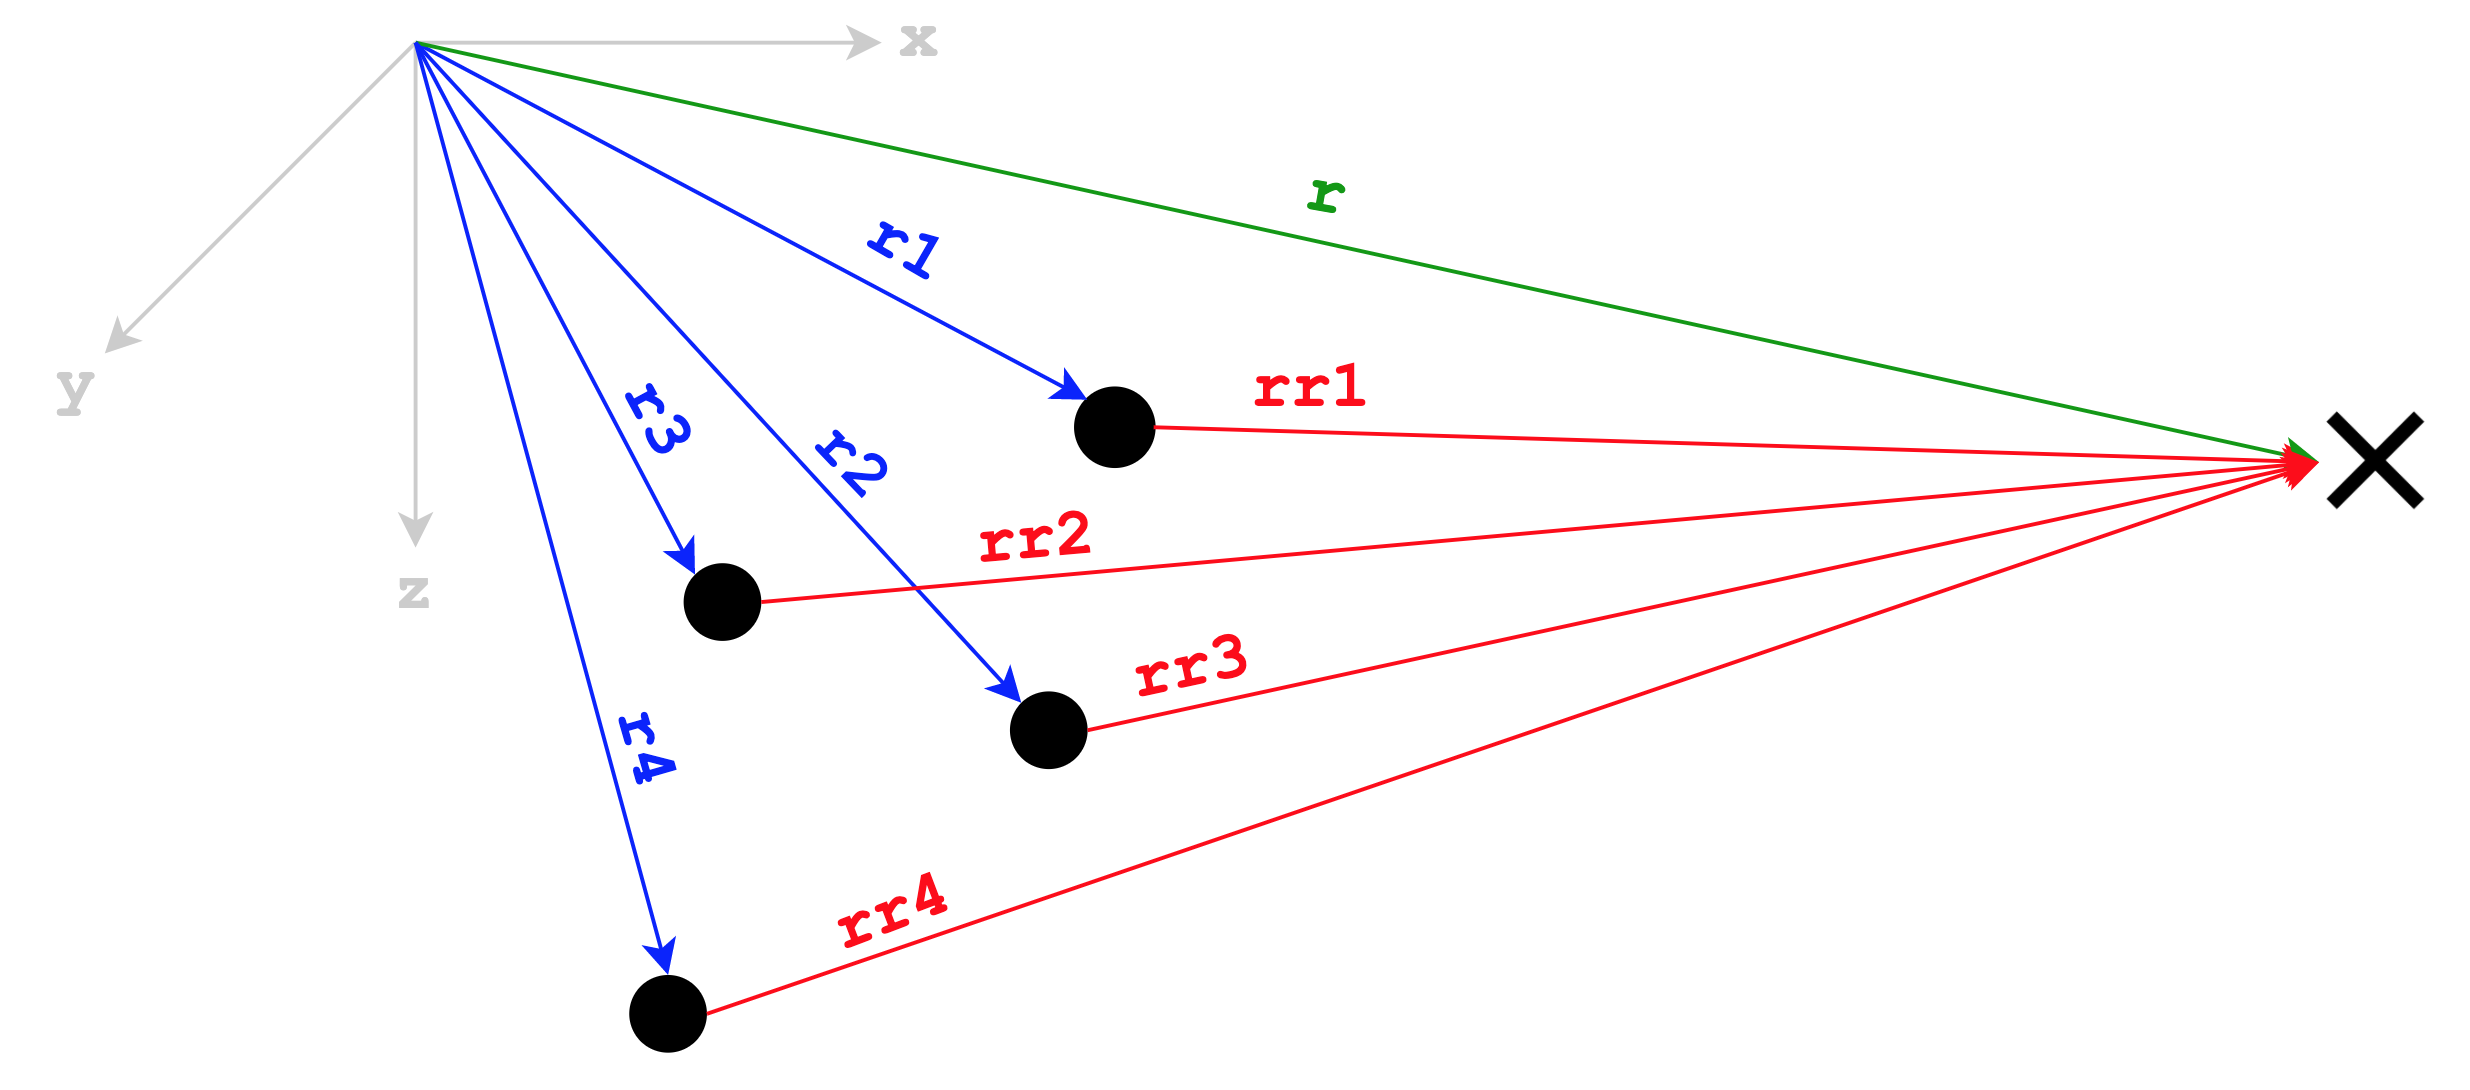
\includegraphics[width=0.8\textwidth]{figures/AoA-init}
	\captionsetup{justification=centering,margin=2cm}
	\caption{Considered scheme for angle of arrival estimation}
	\label{fig:AoA-init}
\end{figure}

Then we can define the times of arrival to each hydrophone as \ref{eq:toa-4h}, where $t_0$ is the absolute time of emission, $c_s$ is the underwater sound speed and $\rho_i$ is the norm of $rr_i$, \ref{eq:rho}, which translates to the distance from hydrophone $i$ to the acoustic source. 

\begin{eqnarray}
& t_i = t_0 +  \frac{\rho_i}{c_s}
\label{eq:toa-4h}
\end{eqnarray}

 However, as explained in the previous section, instead of using the absolute ToA in each hydrophone by computing the expression \ref{eq:toa-4h} for each of them, it can be expressed as a function of a single reference ToA. A simple logic was applied in order to determine this reference hydrophone, which starts by identifying the closest to the acoustic source. This allows to obtain all relative times of arrival by adding the defined reference time to each  between a hydrophone and the reference one. This is achieved by analyzing the  of each pair, $ \Delta t_{ij}$, for all possible combinations of two among four hydrophones, making up a total of six combinations. Considering each hydrophone pair $ij$ with $i, j= \{1,2,3,4\}$ :
 
 \begin{itemize}
 	\item if $ \Delta t_{ij}$ is positive, then hydrophone $i$ is closer to the acoustic source
 	\item if $ \Delta t_{ij}$ is negative, then hydrophone $j$ is closer to the acoustic source
 	\item if $ \Delta t_{ij}$ is zero, then $i$ and $j$ hydrophones are equidistant to the acoustic source
 \end{itemize}
 
Considering these relations, it is possible to compose a vector that accumulates the closer hydrophone between each pair for a certain position of the acoustic source. Extracting the mode of this vector will then return the chosen hydrophone in most cases and therefore the overall closer to the acoustic source. If the closer hydrophones are the equidistant to the source, then it is indifferent which one is selected.  

Thereafter, recalling expression \ref{eq:dist_to_target}, it is possible to write \ref{eq:toa_relation2}, \ref{eq:toa_relation3} and \ref{eq:toa_relation4} which translate the used relations, where  the chose reference sensor is hydrophone 1, for the purpose of exemplification.

\begin{eqnarray}
& T_2 = T_1 + \Delta t_{12} * c_s
\label{eq:toa_relation2}\\
& T_3 = T_1 + \Delta t_{13} * c_s
\label{eq:toa_relation3}\\
& T_4 = T_1 + \Delta t_{14} * c_s
\label{eq:toa_relation4}
\end{eqnarray}

If then the distance $\rho_i$ is raised to the power of two, we know that $||rr_i||^2 = r_i^{T}r_i$, which allows to deduce equation \ref{eq:rho1} after some mathematical manipulation. Considering $\rho_i$ a physical distance, it is also possible to express it trough equation \ref{eq:rho2}, which uses the speed of propagation underwater multiplied by the ToA of the signal from the acoustic source to hydrophone $i$.

\begin{eqnarray}
& \rho_i = ||rr_i|| 
\label{eq:rho}\\
&\rho_i^{2} =  r^{T}r + 2r^{T}r_i + r_i^{T}r_i
\label{eq:rho1}\\
&\rho_i^{2} = c_s^{2} (t_i-t_0)^{2}
\label{eq:rho2}
\end{eqnarray}

Since two distinct relations are defined for $\rho_i^{2}$, then it is possible to consider the algebraic expressions as equivalent, thus forming a single equation to be resolved with only one unknown variable. After some mathematical manipulation, the matrix relation \ref{eq:AoA-matrix} is achieved, where $r$ is isolated and can be estimated.

\begin{eqnarray}
\begin{bmatrix}
1 & 2\: r_i^{T}
\end{bmatrix}
\begin{bmatrix}
r^{T} r \\
r
\end{bmatrix}
=  
\begin{bmatrix}
c_s^{2} (t_i-t_0) - r_i^{T} r_i
\end{bmatrix}
\label{eq:AoA-matrix}
\end{eqnarray}
 
In order to resolve this system of equations and isolate $r$, the least squares method is applied. If \ref{eq:AoA-matrix} is extended to the four considered hydrophones, we obtain matrix $A$ represented as \ref{eq:A} and $Y$ equivalent to \ref{eq:Y}. It is important to notice that the $A$ matrix has to be invertible, thus the rows which contain the chosen hydrophone configuration have to be linearly independent. The least squares method is then expressed as \ref{eq:least-square}, where $X \in \mathbb{R}^{4}$ holds the Cartesian result of $r$. As the method formulates four equations that are meant to calculate only three coordinates, $X$ will contain a fourth element that consists on a nonlinear component equivalent to $||r||^{2}$.

\begin{eqnarray}
& A = 
\begin{bmatrix}
1 & 2\: r_1^{T}\\
1 & 2\: r_2^{T}\\
1 & 2\: r_3^{T}\\
1 & 2\: r_4^{T}
\end{bmatrix}
\label{eq:A}
\end{eqnarray}

\begin{eqnarray}
& Y = 
\begin{bmatrix}
c_s^{2}\: (t_1-t_0)^2 - r_1^{T} r_1\\
c_s^{2}\: (t_2-t_0)^2 - r_2^{T} r_2\\
c_s^{2}\: (t_3-t_0)^2 - r_3^{T} r_3\\
c_s^{2}\: (t_4-t_0)^2 - r_4^{T} r_4\\
\end{bmatrix}
\label{eq:Y}
\end{eqnarray}

\begin{eqnarray}
& X = (A^{T}*A)^{-1}*A^{T}*Y
\label{eq:least-square}
\end{eqnarray}

After infer the Euclidean vector $r$, it is possible to obtain both the bearing trough its direction, $\hat{\boldsymbol{r}}$, and the range through its magnitude, $||r||$.

\subsection{Accuracy analysis}  \label{subchap:acc-analy}

A methodology was formulated in order to evaluate the accuracy that the estimator can achieve in defined circumstances. For this initial approach to the study, the following conditions are considered: 

\begin{enumerate}[label=\alph*)]
	%--------------------
	\item \textbf{Sensor Configuration}  
	
	Each hydrophone configuration is analyzed individually. It is a parameter to be always defined and known from the begging of each simulation.
	
	%--------------------
	\item \textbf{Reference axis}
	
	 The origin of the reference axis is defined at the center of mass of the structure where the hydrophones are fixed, which in this case is the AUV.
	
	%--------------------
	\item \textbf{Injected error} 
	
	In order to make the study more realistic, an $e_i$ error is added to the time differences of arrival, $ \Delta t_{ij}$. These errors are mutually independent and follow a Gaussian distribution with zero mean and a configurable variance of $\sigma^{2}$, i.e., $e_i \sim \mathcal{N}(0,\,\sigma^{2})$. 
	
	 For the simulations performed in this project, a deviation of 5$^{\circ}$, or a window of $[-2.5^{\circ},2.5^{\circ}]$, in the angle of arrival estimation was considered to be reasonable for an underwater navigation scenario. Therefore, since the specified period of the signal is $T = \frac{1}{24400}$ and one period corresponds to a 360$^{\circ}$ phase shift, then the 5$^{\circ}$ will be equivalent to $\frac{5^{\circ}}{360^{\circ}}*T$ which is approximately a deviation of $0.5\mu s$. Hence the considered standard deviation $\sigma$ of the error $e_i$ in the computed time differences of arrival is equal to $0.5\mu s$.
	 
	 %--------------------
	 \item \textbf{Acoustic source position} 
	 
	 The considered positions for the acoustic source, $s$, are originally defined in spherical coordinates, $s_{sph}$. Thus the norm, $n$, corresponds to the source's range in meters, whereas the azimuth, $\phi$, and elevation, $\theta$, define the angle of arrival of the received signal in degrees. Additionally, when these positions are mentioned in Cartesian coordinates throughout the document, they will be referenced as $s_{cart}$.
	 
	 Recalling the definition of spherical coordinates, it is known that for elevations of -90$^{\circ}$ or 90$^{\circ}$, the azimuth angle is meaningless and should not be considered. Since this system is affected by a Gaussian error, then the estimated azimuth angle is expected to return large errors not only for the absolute mentioned elevation values but for a considerable interval around it, dependent on the injected deviation. For that reason, the elevation values are limited to an interval between -80$^{\circ}$ and 80$^{\circ}$ so that the evaluated metrics present a result that is not so reflective of the errors originated from this phenomenon.
	 
	 The positions to be estimated are contained in a matrix with a number of columns equal to the number of positions and three rows consisting of its spherical coordinates. The matrix is arranged so that for each defined norm, the elevation component covers the interval [-80$^{\circ}$ to 80$^{\circ}$] in steps of one and, for each elevation value, the azimuth component covers the interval [-180$^{\circ}$, 180$^{\circ}$] in steps of one, forming partial spheres around the reference axis' origin.

	%--------------------
	\item \textbf{Propagation speed}
	
	In all performed simulations, the considered speed of sound is $1500 \; m/s$, which corresponds to the underwater propagation velocity of waves in typical conditions.
	
\end{enumerate}

Having the conditions enumerated, the logic of the algorithm occurs as follows. For every defined position of the acoustic source, $s$, a function that consists on the estimator is called, receiving as input the $s$, the positions of the hydrophone configuration, $r_i$, and an injected error in the . It then returns the estimated position of the source in Cartesian coordinates, $[x,y,z]$, and in spherical coordinates, $[n, \phi, \theta]$. As the position $s$ in Cartesian corresponds to the real value that is intended to be estimated, we can also obtain the real spherical coordinates by directly converting $s$ using the Cartesian to spherical relations in \ref{eq:cart2sph}.

\begin{eqnarray}
\begin{cases} 
n =  \sqrt{x^2 + y^2 + z^2}\\ 
\phi  = arctan \frac{y}{x}\\ 
\theta =  arctan \frac{\sqrt{x^2+y^2}}{z}
\end{cases}
\label{eq:cart2sph}
\end{eqnarray}

Consequently all conditions are met to analyze the achieved error in each coordinate by comparing the real position to the estimated values as \ref{eq:error1}, where the tested coordinates are $x, y, z, n, \phi$ and $\theta$.

\begin{eqnarray}
&error_{coordinate} = |estimated_{coordinate} - real_{coordinate}|
\label{eq:error1}
\end{eqnarray}

The metrics used to evaluate the quality of the estimator were :

\begin{itemize}
	\item \textbf{Mean squared error} (MSE): Incorporates both the variance and the bias of the estimator, indicating its overall quality
	
	\item \textbf{Standard deviation of the error} ($\sigma$) : Indicates how disperse are the estimates from the expected value
	
	\item \textbf{Minimum error ($min(e_i)$)} : Indicates the minimum error that is obtained by the estimator, thus the best absolute precision achieved
\end{itemize} 

\subsection{Simulations}

A series of simulations were performed in order to understand the behavior and capabilities of the estimator and analyze its overall accuracy.

To illustrate a scenario where this estimator is applicable, we can consider that a vehicle is moving towards an acoustic signal transmitter whose position is unknown. Imagining that the target is at a considerable distance, then the main focus is to achieve an optimal bearing estimation which provides a more direct path and saves resources. The range estimation serves as secondary measurement that indicates how near the vehicle is from the destination, so that it is possible to make control decisions such as moderate the navigation speed in the proximity of the target. For the reasons outlined, the study that follows presents a more thorough analysis of the azimuth and elevation errors. 

In this section, three different hydrophone configurations are considered, A, B and C defined in \ref{tab:configs_test1}, where the columns $r_{Ai}$, $r_{Bi}$ and $r_{Ci}$ contain the position's coordinates of each hydrophone $i$.

\begin{table}[!htbp] %use H to adjust
	\begin{center}
		\begin{tabular}{ l | c c c c | c c c c | c c c c}
			%\hline
			%\multicolumn{1}{c|}{} & \multicolumn{4}{c|}{A} & \multicolumn{4}{c|}{B} \\
	    	\toprule
	       % \cline{2-9}
			\multicolumn{1}{c|}{} & $r_{A1}$ & $r_{A2}$ & $r_{A3}$ & $r_{A4}$ & $r_{B1}$ & $r_{B2}$ & $r_{B3}$ & $r_{B4}$ & $r_{C1}$ & $r_{C2}$ & $r_{C3}$ & $r_{C4}$ \\
			\midrule
			\multirow{1}{0.5em}{x} 
			& 0.02 & 0.02 & 0 & 0 & 0.1 & 0.1 & 0 & 0 & 0.1 & 0 & 0 & 0  \\
			%\hline 
			\multirow{1}{0.5em}{y} 
			& 0 & 0 & 0.1 & -0.1 & 0 & 0 & 0.1 & -0.1 & 0 & 0 & -0.0707 & 0.0707 \\
			%\hline 
			\multirow{1}{0.5em}{z} 
			& 0.1 & -0.1  & 0 & 0 & 0.1 & -0.1  & 0 & 0 & 0 & 0.1 & -0.0707  & -0.0707\\
			\bottomrule 
		\end{tabular}
		\caption{Hydrophone configurations used for accuracy tests}
		\label{tab:configs_test1}
	\end{center}
\end{table}

For the data visualization, two essential types of representation were developed :

\begin{itemize}
	\item A 2D static representation of the error per position $s$. The errors to be tested are coordinates $x, y, z$, norm, azimuth angle or elevation angle.
	
	\item A 3D map of the obtained error. The x-axis holds the azimuth angle in degrees, the y-axis holds the elevation angle in degrees and the z-axis represents the measurement of a chosen parametric error. This allows to visualize, for a chosen configuration, how the estimation quality evolves in space. Since this representation in static form is not clear, it will not be illustrated in the course of this document. 
	
\end{itemize}

For the first simulation, configuration A is tested for the acoustic source positions previously described, in a total of 58121. The obtained plots for a norm equal to 10 meters are illustrated in \ref{fig:s1-A-n10-sph}, representing the error obtained by this specific configuration for all positions of the acoustic source.

\begin{figure}[!htbp]
	\makebox[\textwidth][c]{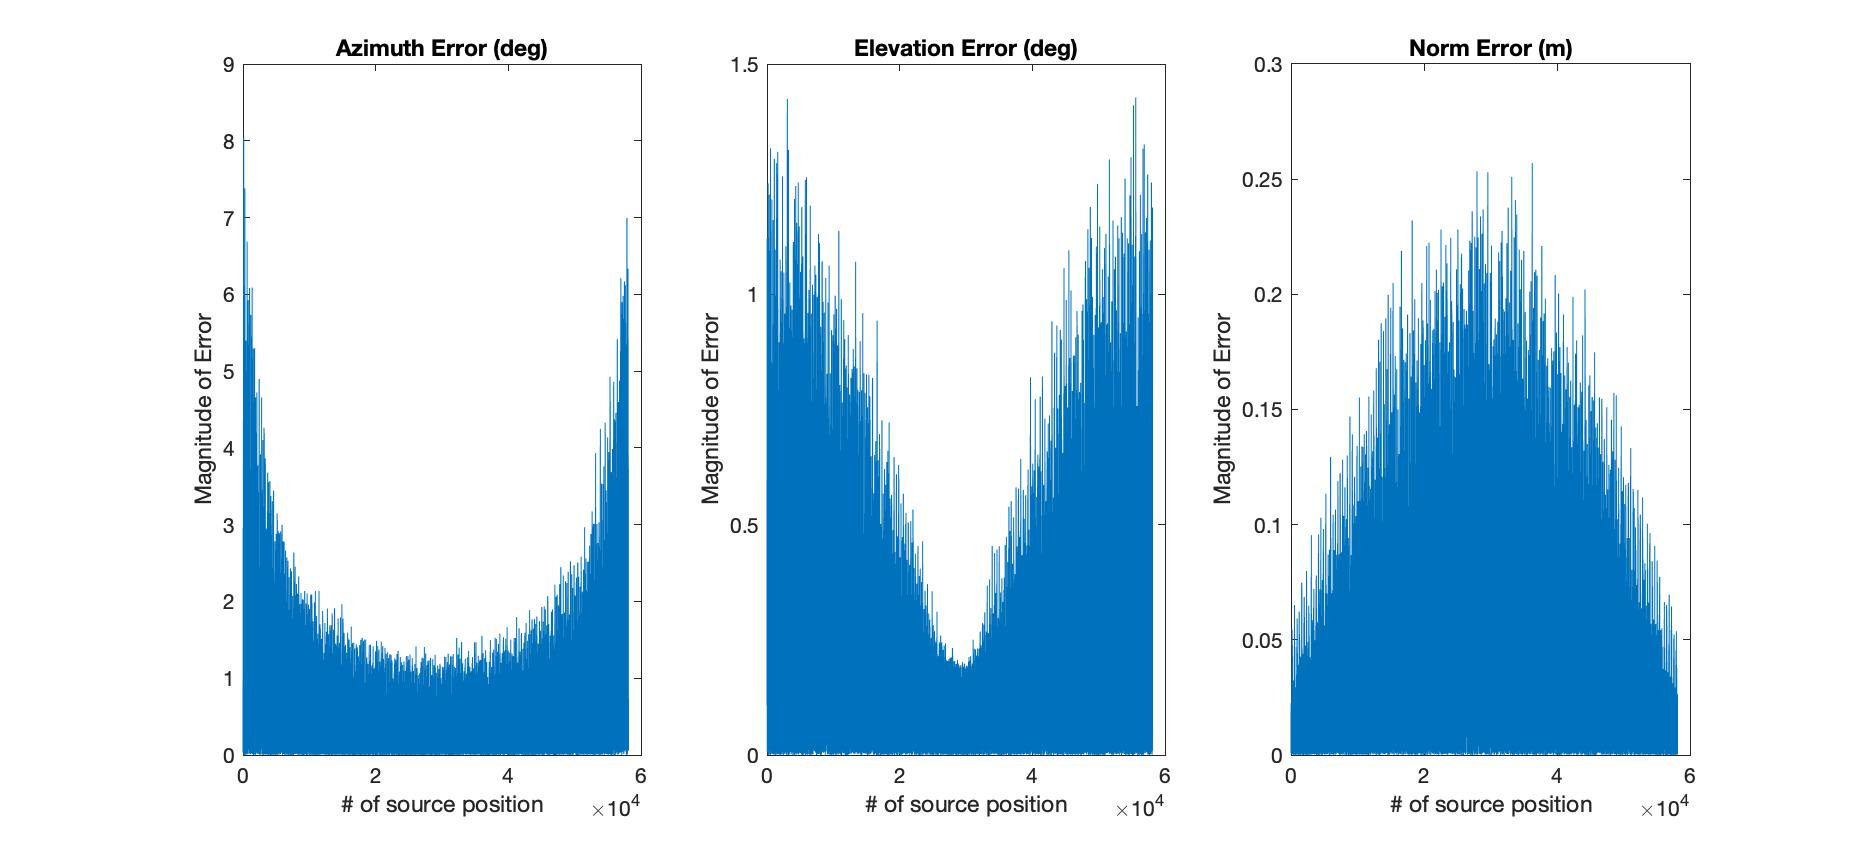
\includegraphics[width=1.1\textwidth,height=0.35\textheight]{figures/plot-s1-A-n10}}
	\captionsetup{justification=centering,margin=2cm}
	\caption{Plots of azimuth, elevation and norm errors for defined source positions}
	\label{fig:s1-A-n10-sph}
\end{figure}

Upon simulation, it is possible to observe that since the configuration is symmetrical in relation to the x-axis, the graphics demonstrate a pattern which evolves from the limits, where the elevation values are closer to the thresholds, towards the middle where the elevation angles are closer to zero. The positions between 28881 and 29241 correspond to elevation angles of $0^\circ$.

Accordingly, some conclusions can be drawn about configuration A from the obtained results. For positions with elevation angle close to its range limits, a deviation in the estimate causes higher azimuth error since the depth of the baseline along the x-axis is decreased from the transmitter's point of view as the elevation slope increases. Additionally, since the configuration has a shorter baseline along the x-axis, then the elevation is more precisely estimated in positions that are approximated to angles around the configuration's geometric center. As observable, the norm error achieves a maximum of $0.25m$, which corresponds to approximately 2.5\% from the original norm. 

For the same conditions, the resulting $x, y$ and $z$ errors are illustrated in \ref{fig:s1-A-n10-cart}. As can be observed, for a range of 10 meters the maximum errors achieved are: for $x$ $\approx$ $0.28m$, for $y$ $\approx$ $0.037m$ and for $z$ $\approx$ $0.038m$. It should be pointed out that there is a higher error in the $x$ coordinate, which corresponds to the direction of the shorter baseline that consequently originates a greater uncertainty. Additionally, there is a decrease on the $y$ error for lower elevation angles and, in elevation angles between $-45^{\circ}$ and $45^{\circ}$, the $z$ coordinate presents higher estimation error, which are both limitations caused by the configuration's symmetry as well.

\begin{figure}[!htbp]
	\makebox[\textwidth][c]{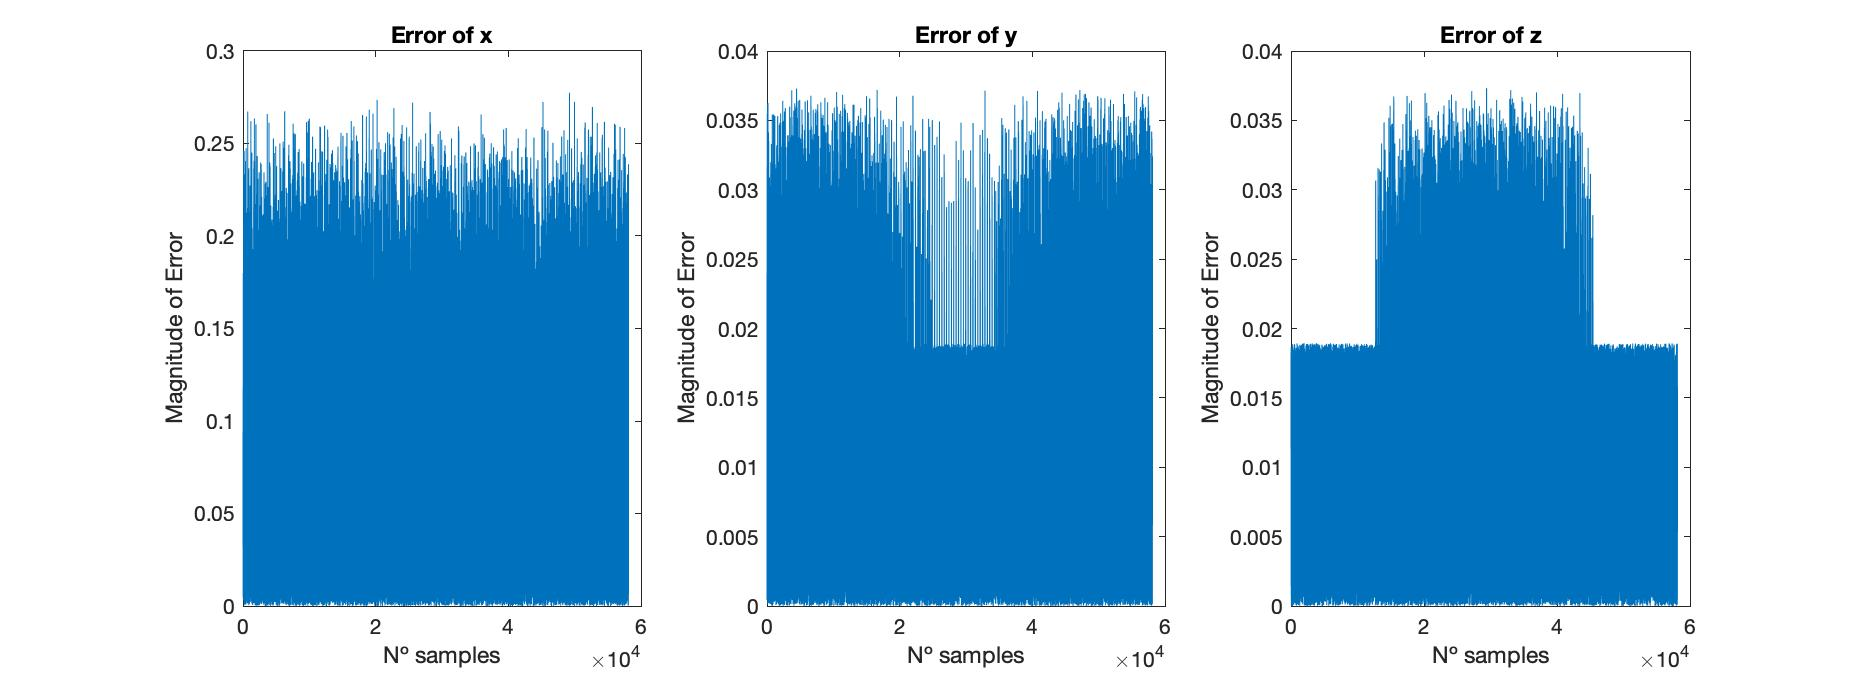
\includegraphics[width=1.1\textwidth,height=0.3\textheight]{figures/plot-cart-A-n10}}
	\captionsetup{justification=centering,margin=2cm}
	\caption{Plots of $x, y$ and $z$ errors for defined source positions}
	\label{fig:s1-A-n10-cart}
\end{figure}

It should be noted that the chosen configuration A for the former analysis is by no means an optimal solution for the estimation. This particular layout was selected because it emphasizes several system responses to distinct configuration characteristics, allowing to understand how should it be adapt to achieve better results.

In order to further analyze the influence of the hydrophones placement in the estimation and which design choices lead to better estimations, two more scenarios are considered to test different aspects:

\paragraph{Influence of range in estimation} In order to compare the range influence on the estimation, a second simulation intends to test the same configuration for a norm of 100 meters. The azimuth and elevation estimations do not demonstrate any visible changes in terms of range and the norm error increases for a maximum of $2.65m$, which still corresponds to approximately 2.6\% error from the original norm. However, the $x, y$ and $z$ estimation demonstrate an error increase of about 10 times, since a small deviation in angle can correspond to a large difference in Cartesian coordinates. Nonetheless, for increasing ranges these errors stay proportional, so the error percentage is similar in any range. This phenomenon is illustrated in \ref{fig:cart-range}, where the error in $x$ increase approximately 10 times for norms equal to $10 m$, $100 m$ and $1000 m$.

\begin{figure}[!htbp]
	\makebox[\textwidth][c]{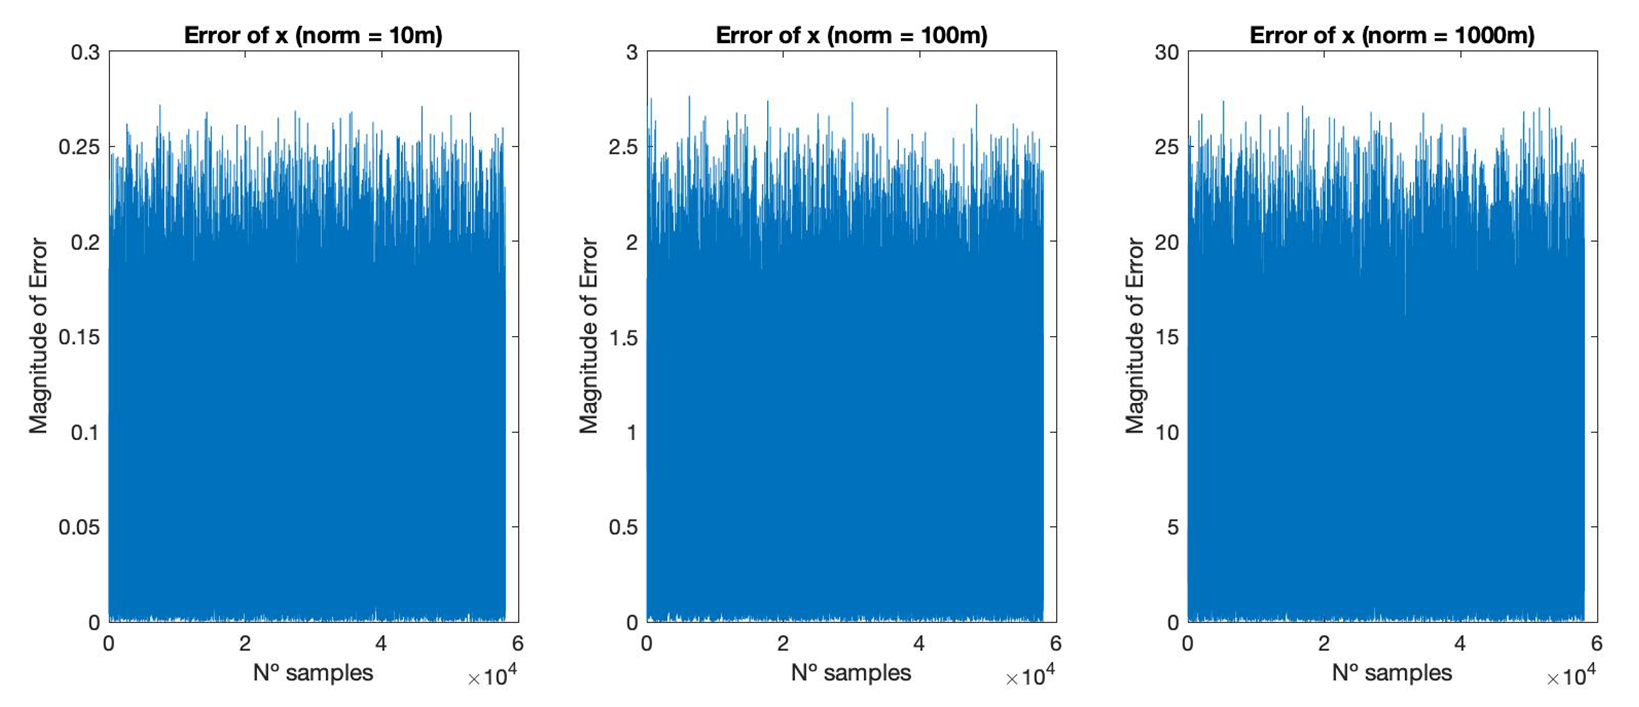
\includegraphics[width=1\textwidth]{figures/plot-cartesian-range}}
	\captionsetup{justification=centering,margin=2cm}
	\caption{Evolution of error in Cartesian coordinates for increasing norms}
	\label{fig:cart-range}
\end{figure}

\paragraph{Increasing the shorter baseline} Since there are some issues that can be observed due to the short baseline along the x-axis, a third simulation serves to understand the influence of increasing this baseline in the estimation. Therefore, the baseline is increased by employing configuration B. After the simulation, the errors decreased visibly, which are indicated in \ref{tab:azimuth-test1}.

\paragraph{}

%\begin{enumerate}
%	\item \textbf{Influence of range in estimation}: In order to compare the range influence on the estimation, a second simulation intends to test the same configuration for a norm of 100 meters. The azimuth and elevation estimations do not demonstrate any visible changes in terms of range and the norm error achieves a maximum of 2.65, which still corresponds to approximately 2.6\% error from the original norm. However, the $x, y$ and $z$ estimation demonstrate an error increase of about 10 times. This indicates that the estimation in Cartesian coordinates is much more affected for long ranges, since a small deviation in angle can correspond to a large deviation in cartesian coordinates.
%	although the error does not influence the angle estimation, the absolute value is affected 
%	
%	\item \textbf{Increasing the shorter baseline}: Since there are some issues that can be observed due to the short baseline along the x-axis, a third simulation serves to understand the influence of increasing this baseline in the estimation. Therefore, the baseline is increased by employing configuration B. After the simulation, the errors decreased visibly, which are indicated in \ref{tab:azimuth-test1}.
%\end{enumerate}

%-----------------
After analyzing a specific configuration which demonstrate various limitation due to its arrangement design, it is desirable to compare it with different hydrophone placements. Therefore, table \ref{tab:azimuth-test1} contain the achieved results of MSE, standard deviation and minimum error for azimuth and elevation estimation in degrees, using norms equal to 10 and 1000 $m$ for configurations A, B and C. Configuration A represents an almost flat structure, configuration B is a variation of A with an increased depth and configuration C resembles an AUV shape. By inspection it is possible to conclude that configuration B returns the lowest standard deviation and MSE, as it is also the one with the larger baselines between sensors.

\begin{table}[!htbp] %use H to adjust
	\begin{center}
		\makebox[\textwidth]{
		\begin{tabular}{ c | c c | c c | c c}
			%\hline
			\toprule
			\multicolumn{3}{c|}{} & \multicolumn{2}{c|}{Azimuth} & \multicolumn{2}{c}{Elevation}  \\
			\midrule
			% \cline{2-9}
			\multicolumn{1}{c|}{Configuration} & Norm & MSE & Standard Dev & Minimum & Standard Dev & Minimum \\
			\midrule
			\multirow{2}{*}{A} &10 & 0.544 & 0.605 & 8.743$\times10^{-7}$ & 0.186 & 3.103$\times10^{-6}$\\
		%	&100 & 0.5465 & 0.6090 & 6.0529$\times10^{-6}$\\
			&1000 & 0.542 & 0.599 &  8.378$\times10^{-6}$ & 0.185 & 5.059$\times10^{-6}$\\
			\midrule	
			\multirow{2}{*}{B} &10 & 0.161 & 0.143 & 1.21$\times10^{-6}$ & 0.050 & 3.456$\times10^{-6}$\\
			&1000 & 0.161 & 0.144 & 1.494$\times10^{-6}$  & 0.050 & 4.910$\times10^{-7}$\\
			\midrule			
			\multirow{2}{*}{C} &10 & 0.230 & 0.213 & 1.305$\times10^{-5}$  & 0.067 & 2.790$\times10^{-5}$\\
		%	&100 & 0.2304 & 0.2119  & 4.3874$\times10^{-6}$\\
			&1000 & 0.223 & 0.212 & 4.096$\times10^{-6}$  & 0.066 & 4.394$\times10^{-6}$\\
			\bottomrule 
		\end{tabular}}
		\caption{Comparison of obtained errors for different configurations}
		\label{tab:azimuth-test1}
	\end{center}
\end{table}

Having explored the behavior of the estimator in specific conditions, there are still factors which were not discussed that may influence the system's performance or lead to an improvement. Therefore, four main ideas will be explored regarding the influence of the numeric quantization on the estimation accuracy, weather the absolute ToA is absolutely necessary for the position estimation, how is the estimates' dispersion for a specific position due to the injected error and the influence of increasing the baseline to the estimation accuracy.

\subsubsection{Influence of numeric quantization on accuracy}

The first term to be analyzed is how much does the quantization of the calculations influence the obtained accuracy of the estimator. In order to analyze this, a simple adaptation was made to the numeric precision of the TDoA values that are input of the system. Instead of using the MATLAB precision of fifteen decimal places, the value was truncated to a specified number of decimal places, $\kappa$.
Since the time differences of arrival have magnitudes around microseconds, then initially they are multiplied by $10^6$ to avoid missing information. Then the relation \ref{eq:trucate} is applied resulting in a truncated value with $\kappa$ decimal places. Finally after the truncation, the value is converted again to seconds to be used in the algorithm.

\begin{eqnarray}
&_{truncated} = \frac{round(*2^{\kappa})}{2^{\kappa}};
\label{eq:trucate}
\end{eqnarray}

To evaluate the influence of the truncation in the estimation, configuration C is used to test a norm equal to 10. The original measurements are already represented previously. For a $\kappa$ of one decimal place, the azimuth standard deviation is 0.261 degrees, the elevation standard deviation is 0.087 degrees, the norm standard deviation is $0.014m$ and the MSE is 0.272. Overall, the estimation errors increase but, in practical terms, the truncation causes near to any difference in the estimation. 

Since one decimal place does not bring too much discrepancy, the limit case is tested where zero decimal places are considered. In this case, the azimuth standard deviation is $0.416^{\circ}$, the elevation standard deviation is $0.136^{\circ}$, the norm standard deviation is $0.0209m$ and the MSE is 0.439. As observed, the estimations are more influenced, however they still do not compromise the reliability of the estimation.

\subsubsection{Impact of ToA measurement on position estimation}

As previously mentioned, the estimator uses the approximation explained in \ref{subsubsec:toa-approx} which allows all hydrophones to use the same reference ToA added by a TDoA, representing the full distance between each hydrophone and the transmitter. However, for long range positions the ToA is consequently much larger in relation to the time differences of arrival. So, the hypothesis is that for these cases the ToA is irrelevant for the calculations and the TDoAs can be used alone to estimate the angle of arrival.

In order to simulate this, the calculated reference time is substituted by $\frac{10^4 m}{1500 m/s}$, which corresponds to a distance of $10 km$. The results demonstrated no visible change in the error of the estimate. However, for distances bellow $100m$ the impact of this approximation starts to be noticed. Therefore, it is considered that the hypothesis is valid. 

\subsubsection{Analysis of estimates' dispersion due to injected error}

So far, the errors that have been analyzed correspond to a random executed simulation, which is influenced by an injected error equivalent to $5^{\circ}$. If the exact same experiment is executed several times, although the returned values have the same magnitude, they are only similar and rarely the same. Therefore, if each estimation is repeated a defined number of times, then the estimates can be analyzed so that it is possible to extract a single mean value which translates the estimation error.

In order to simulate this mechanism, an adaption was introduced in the previous algorithm. For each transmitter position $s$, the estimation is reiterated a specified number of times and, in each round, the azimuth and elevation errors are accumulated. After all samples are collected for a specific position, the azimuth/elevation deviation is calculated as the standard deviation of the accumulated azimuth/elevation errors and the azimuth/elevation errors are considered to be the mean of the accumulated azimuth/elevation errors. After the measurements are executed for every position in space, it is computed the overall azimuth and elevation errors and deviations which characterize the specific chosen configuration, as well as the final MSE.

For exemplification purposes, configuration C was tested 100 consecutive times with no reiterations for each position, \ref{fig:plot-accum0}, and with 100 accumulated samples, \ref{fig:plot-accum100} in order to verify the dispersion of the obtained results. As it is observed, when the error is averaged with accumulated samples, there is a smaller discrepancy among the results.

\begin{figure}[!htbp]
	\makebox[\textwidth][c]{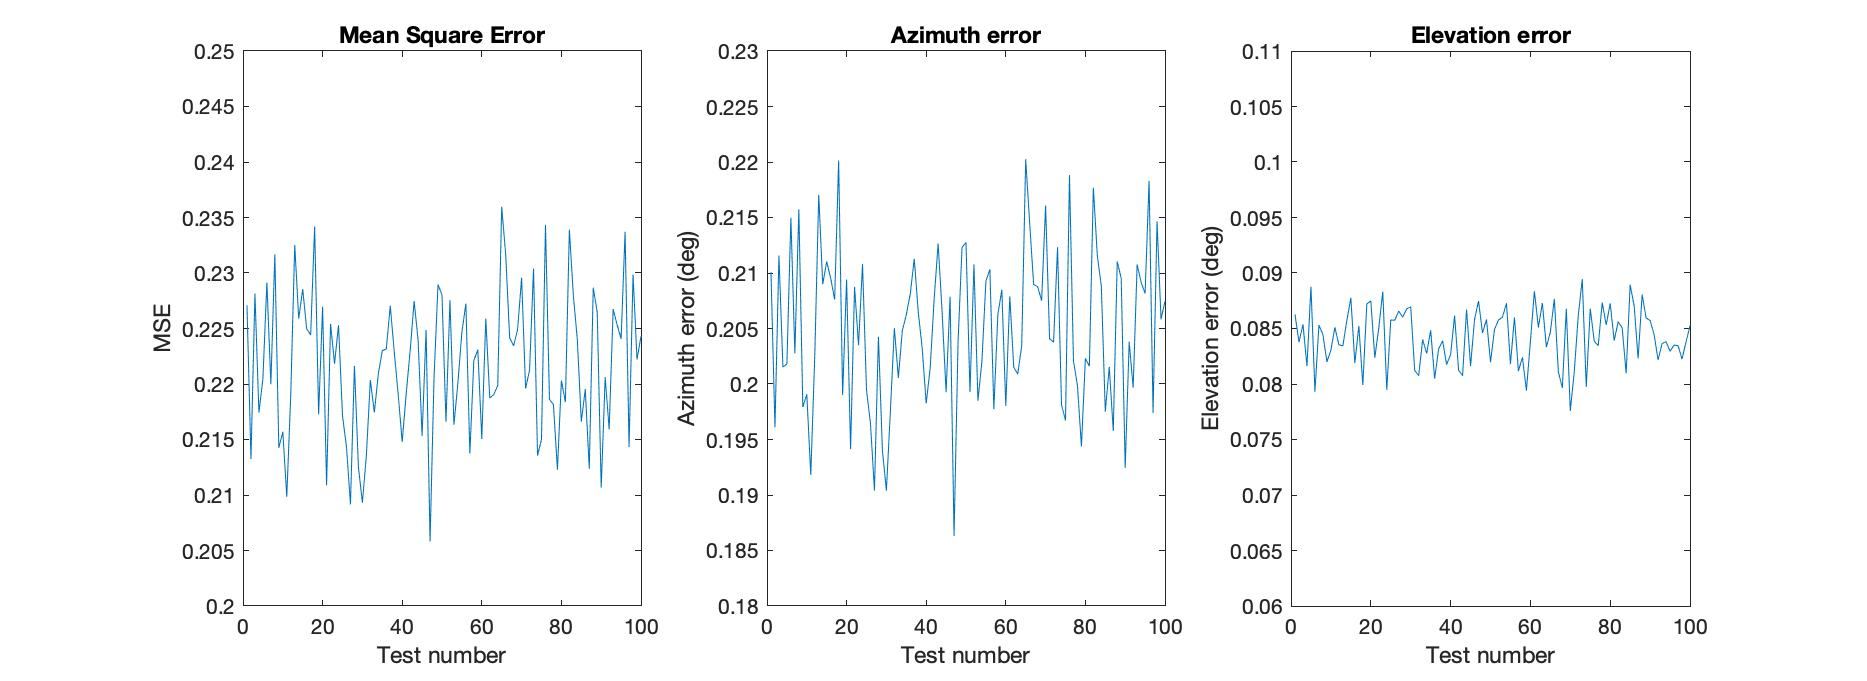
\includegraphics[width=0.9\textwidth]{figures/plot-accum0-dev0-100times}}
	\captionsetup{justification=centering,margin=2cm}
	\caption{Obtained error for a single configuration with no accumulated samples}
	\label{fig:plot-accum0}
\end{figure}

\begin{figure}[!htbp]
	\makebox[\textwidth][c]{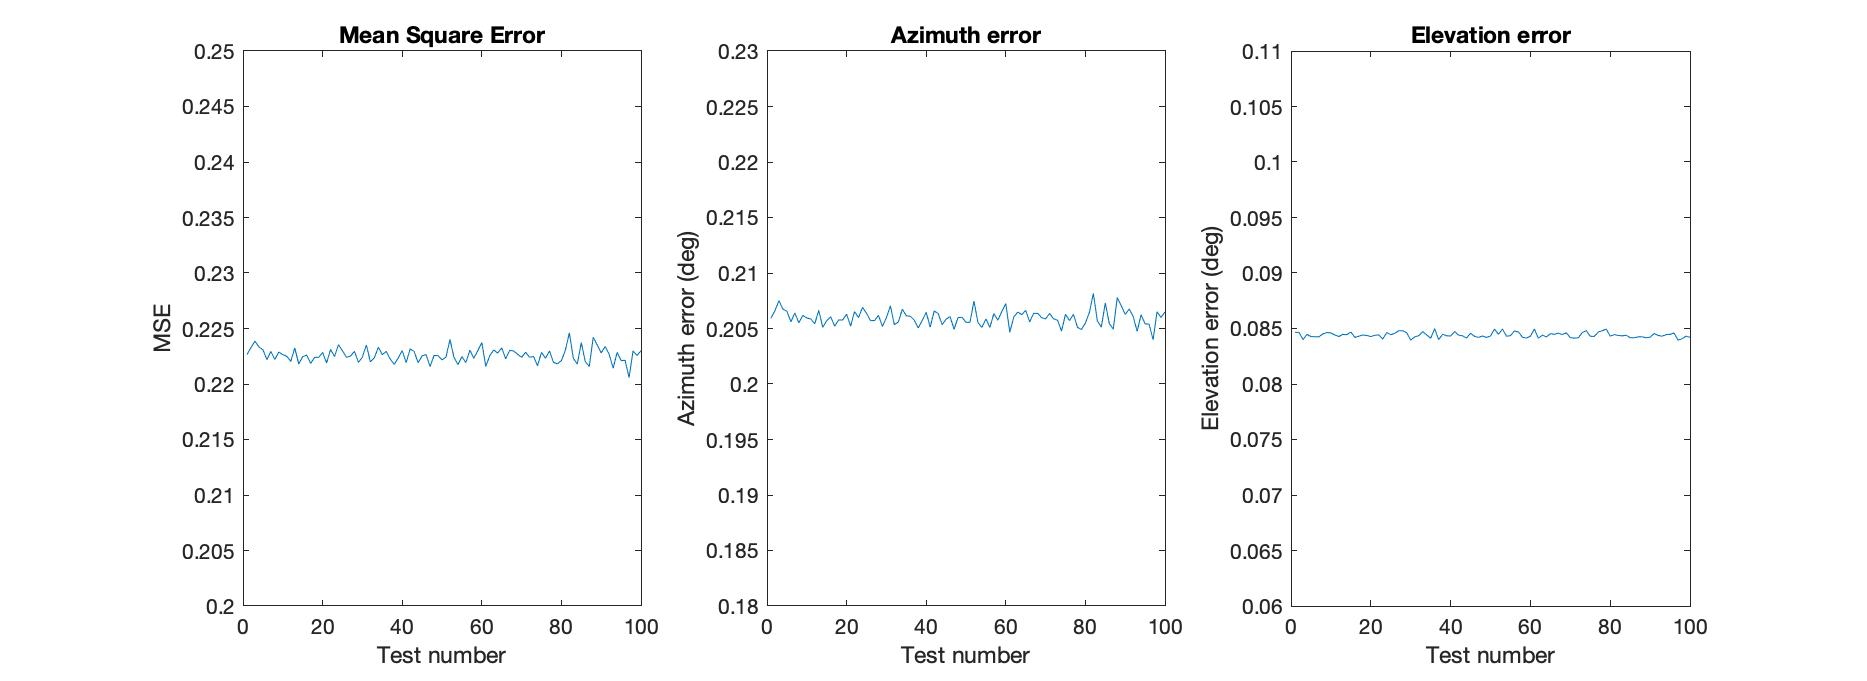
\includegraphics[width=0.9\textwidth]{figures/plot-accum100-dev0-100times}}
	\captionsetup{justification=centering,margin=2cm}
	\caption{Obtained error for a single configuration with 100 accumulated samples}
	\label{fig:plot-accum100}
\end{figure}

This approach allows to achieve more coherent results and to characterize the configurations in a more methodical manner.

\subsubsection{Influence of increasing the configuration baseline}

Until this point, there are several mentions to the baseline of the used configuration and its numeric impact on the estimation performance. However, there are no conclusions about the optimal baseline that should be used. The goal of this test is to delineate the influence of increasing the hydrophones' baseline in the obtained error. 

In order to execute this test, configuration C is used as well as the method previously explained that reiterates each estimation a defined number of times to achieve average dispersion values. To create an increasing baseline along the tests, in each iteration the $x$ coordinate of $r_{C1}$ increases $0.01 m$ in a total of 200 times, which makes up a displacement range between 0.1 and $2 m$. Each position generates 100 accumulated samples that result in a single measurement per configuration. 

Plot \ref{fig:plot-baseline-increase-1} represents the collected errors for each of the described configurations, whose baseline is progressively increasing in a constant pace. As illustrated, the obtained errors decrease visibly in the first 100 tests, corresponding to a $r_{C1}$ position between 0.1 and $1 m$, becoming considerably constant for further distances.

\begin{figure}[!htbp]
	\makebox[\textwidth][c]{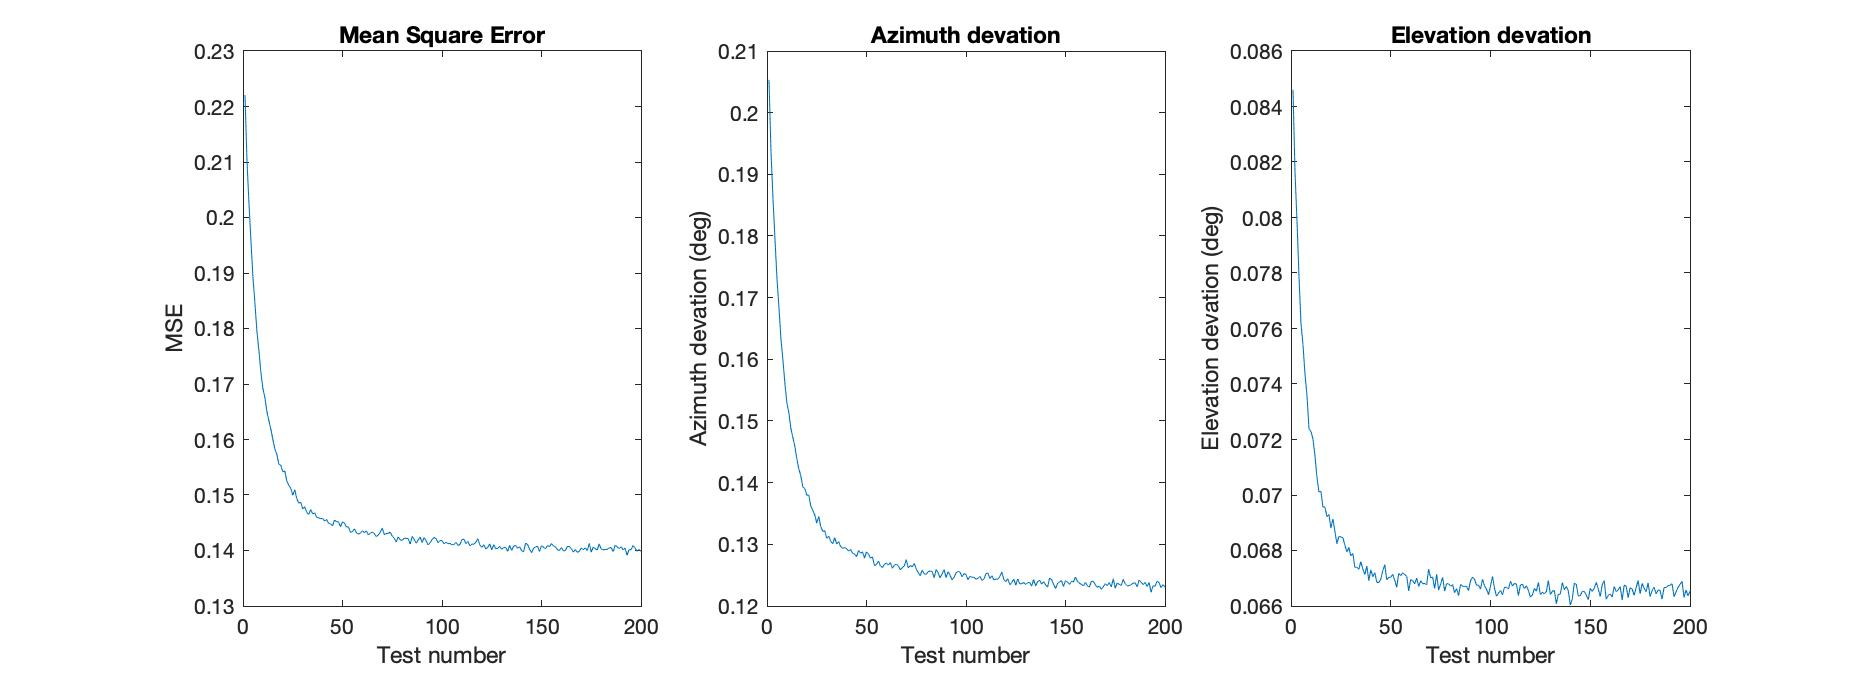
\includegraphics[width=1.1\textwidth]{figures/plot-Hbaseline-dev001-100accum-100s-1}}
	\captionsetup{justification=centering,margin=2cm}
	\caption{Error evolution with increasing baseline for $r_{C1}$}
	\label{fig:plot-baseline-increase-1}
\end{figure}

Additionally, the same experiment was done on hydrophone $r_{C2}$ of the same structure, since its position on the configuration gets a different exposure than $r_{C1}$ and a different outcome is expected. Having considered the same conditions as explained for the previous simulation, figure \ref{fig:plot-baseline-increase-2} illustrates the obtained results. It can be observed that the displacement of this specific hydrophone only causes an estimation improvement in the elevation deviation, it does not affect the estimation of the azimuth deviation and slightly increases the azimuth deviation. Therefore, an estimation improvement may not be achieved by distancing a random hydrophone, a study should be conducted for each particular configuration to determine which displacements lead to an enhancement.

\begin{figure}[!htbp]
	\makebox[\textwidth][c]{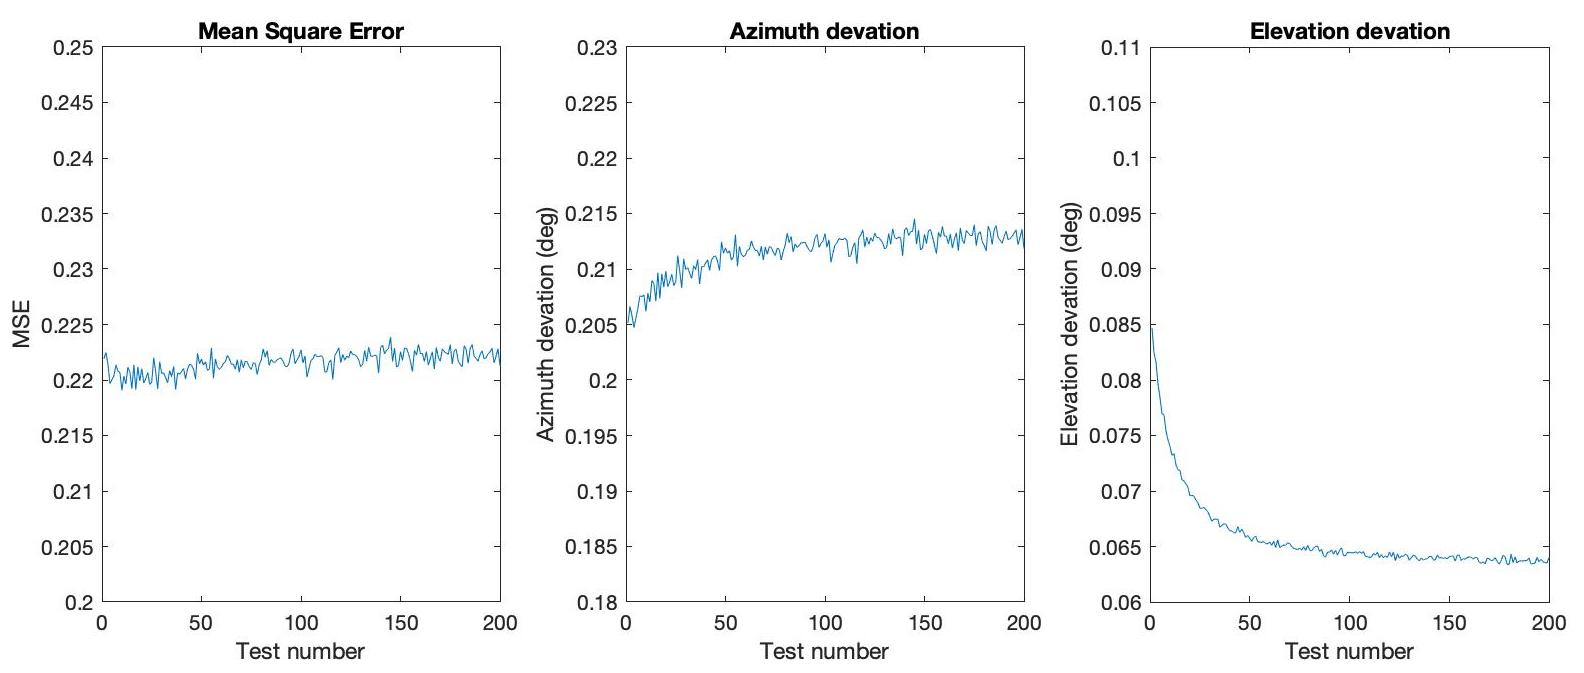
\includegraphics[width=1.1\textwidth]{figures/plot-Hbaseline-dev001-100accum-100s-2}}
	\captionsetup{justification=centering,margin=2cm}
	\caption{Error evolution with increasing baseline for $r_{C2}$}
	\label{fig:plot-baseline-increase-2}
\end{figure}

In conclusion, it is proved that increasing the baseline of a configuration in specific cases may result in a decrement of the overall estimation error. However, this only occurs for a maximum distance after which the error becomes constant. 

\subsection{Conclusions}

The present chapter focused on detailing the developed estimator, including the involved mechanisms and algorithm, a behavioral analysis and characterization based on simulated results. Therefore, by way of summary, some main conclusions can be taken:
\begin{itemize}
	\item The azimuth and elevation errors do not vary with the range of the transmitter's position, in contrast to errors in Cartesian coordinates which increase proportionally with the range;
	
	\item The ToA measurement is not essential for long range distances. So, in those cases there is no need for synchronization since a random large ToA can be used instead;
		
	\item A lower numeric precision in the calculations affects the obtained results, however since in the explored situations the errors are inherently small, the error increase does not have an impact on the system from a practical point of view;
	
	\item Increasing the baseline of a hydrophone configuration can result in a better estimation, until reaching a certain distance after which the error becomes constant. Therefore, when choosing an hydrophone layout which can be limited to the dimensions of a physical structure, it does not have to be sought the maximum baseline possible but the length that leads to the error becoming constant;
	
	\item Applying a reiteration process to create averaged errors for each configuration, creates results which are more consistent thus more capable of characterizing a specific process. Additionally, the random nature of the Monte Carlo approach is attenuated, resulting in more coherent results.
	
	\item The hydrophone configuration is a main factor on the estimation performance for any position in space. Although the characteristics that a configuration should meet to be optimal are still not clear, some aspects can be pointed out: 
	
	\begin{itemize}
		\item It is mandatory to ensure a sensor layout which covers three dimensions, so it is possible to estimate coordinates in 3D;
		\item The positions of the sensors must be linearly independent to allow the application of the least squares method;
		\item It is fundamental to have an adequate baseline which can be determined with the tool previously explained;
		\item Bearing in mind that the configuration may be employed in real scenarios, it is useful to create schematics which require achievable distances between hydrophones and respect logical shapes to install in vehicles such as AUVs.
	\end{itemize}
\end{itemize}
\chapter{Dynamic reconfigurable configuration method}  \label{chap:study}
%Experiments on Localization Reliability and Improvement

Having studied the estimator's behavior for several different configurations and conditions, there is still uncertainty about the best performance it can achieve. In the considered system, the hydrophone configuration has a decisive role on the achieved precision, as demonstrated. Therefore, a way to optimize the system's estimation would be to choose, for each position of the acoustic source, the configuration that returns the best estimation and thus the one that should be employed.

In a field scenario where a vehicle is searching for an acoustic transmitter, as it is navigating and readjusting its trajectory, the relative direction that is being estimated in real time is changing. Therefore, the system's performance can vary and arises the necessity of having different angles of vision from the hydrophones to the target. To resolve this issue, the proposed method assumes that the used USBL system integrates more than four hydrophones placed in known positions. This way, it is possible to dynamically reconfigure which four hydrophones are used at a time leading to an estimation that is optimal for the available sensors. 

Another possibility is to determine through the same techniques which configuration of four hydrophones, tested in various positions along the vehicle, is the overall best for short and long range estimation. This can lead to a moderate compromise of the estimate precision, however decreases the number sensors that are employed and therefore the cost of the system.

This chapter is dedicated to explaining the methodological approach, the main findings and conclusions that were driven from the formulated dynamic reconfigurable configuration method.

\note{descrever mais detalhadamente os temas que vao ser abordados no capitulo}

\note{- tendo em conta a posição do espaço, escolher a melhor configuração\\
	- qual a melhor configuração (ou duas) para curto e longo alcance?\\
	- tendo em conta a configuração qual é o local no espaço que consegue melhor resultados? (cramer rao)}

\section{Monte Carlo Approach} \label{sec:config-perf}

The developed algorithm serves as a tool to determine which is the best available hydrophone configuration for a certain target position. This approach uses a Monte Carlo method which is useful to solve problems that are deterministic in nature through repetition of and experiment with random parameter(s). Additionally,it makes use of the previously developed estimator, which is comprehensively explained in \ref{subsec:estimator}, to estimate the target position for each sensor configuration.
		
For this experiment, it is considered a total of nine hydrophones, whose positions are contained in $matrix_{r_{i}}$, defined by table \ref{tab:config-9h}. Each column expresses the coordinates of each hydrophone, $r_i$, where the value of $x_i$ is in the first row, the value of $y_i$ in the second row and the value of $z_i$ in the third row. Additionally, $q = 0.1$, $w = 0.1$ and $e = \frac{ \sqrt{2}}{2} * w$.

\begin{table}[!htbp] %use H to adjust
	\begin{center}
		\begin{tabular}{c | c c c c c c c c c}
			\toprule
			& r1 & r2 & r3 & r4	& r5 & r6 & r7 & r8	& r9 \\ \hline 
			\multirow{1}{0.5em}{x} 
			& q & 0 & 0 & 0 & 0 & 0 & 0 & 0 & 0\\
			\midrule 
			\multirow{1}{0.5em}{y} 
			& 0 & 0 & 0 & w & -w & e & e & -e & -e\\
			\midrule 
			\multirow{1}{0.5em}{z} 
			& 0 & w & -w & 0 & 0 & e & -e & e & -e \\
			\bottomrule 
		\end{tabular}
		\caption{Position coordinates for an implementation with 9 hydrophones}
		\label{tab:config-9h}
	\end{center}
\end{table}

These positions are arranged so that they can mimic a possible deployment in an AUV, as represented in figure \ref{fig:9h-config}, where hydrophone $r_1$ is placed in front of the vehicle and hydrophones $r_2$ to $r_9$ form a circle with a $10 cm$ radius around the vehicle.

\begin{figure}[!htbp]
	
	\makebox[\textwidth][c]{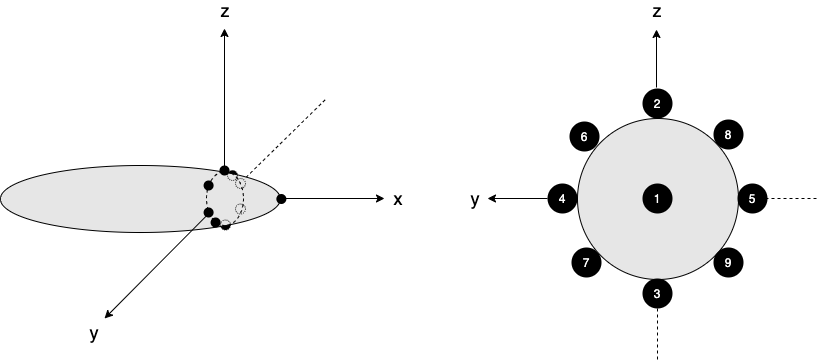
\includegraphics[width=0.8\textwidth]{figures/9h-config}}
	\captionsetup{justification=centering,margin=2cm}
	\caption{Hydrophone positions for an implementation with 9 hydrophones}
	\label{fig:9h-config}
\end{figure}

Since the used configuration has to be three dimensional, it is defined that hydrophone $r_1$ always integrates the configuration as it is the only one in a different plan. Accordingly, the number of possibilities is combinations of three out of eight, $C(8,3)$, making up a total of 56 combinations. Each of these configurations are associated with a number from 1 to 56 and the hydrophones that integrate each of them are outlined in table \ref{tab:long} for consultation when necessary.

Having the system presented, the algorithm will be explained next. For the sake of clarity, the algorithm was outlined in pseudo code and separated into two main parts, where \ref{alg:alg1} is integrated in \ref{alg:alg2}.

\begin{algorithm}
	\setstretch{1.3} 	%increase space between lines
	%\algsetup{linenosize=\scriptsize} 	%adapts font size
	\scriptsize		%makes it smaller, idk
	\caption{Determines the average azimuth errors, elevation errors and MSE for a set of hydrophone configurations}
	\label{alg:alg1}
	\begin{algorithmic}[1]
		\FOR{\texttt{all k configurations}} %k = 1 \textbf{to} n\_config
		\FOR{\texttt{all i estimation repetition}} %i = 1 \textbf{to} accum\_samples
		\STATE\texttt{$estimator(s, config(k), error)$}
		\COMMENT{returns estimate in Cartesian and spherical coordinates}
		\STATE \texttt{accum\_estimate(i) $\gets$ result of the estimator in each repetition} 
		\STATE \texttt{accum\_error\_azimuth(i) $\gets$ azimuth error in each repetition} 
		\STATE \texttt{accum\_error\_elevation(i) $\gets$ elevation error in each repetition} 
		\ENDFOR
		\STATE $mean\_estimate \gets \dfrac{accum\_estimate}{accum\_samples}$
		%\newline
		%\STATE \texttt{Compute the mean and standard deviation of accum\_error\_elevation and accum\_error\_azimuth}
		\STATE
		\STATE $deviation\_azimuth(config) = std(accum\_error\_azimuth);$
		\STATE $deviation\_elevation(config) = std(accum\_error\_elevation);$
		%\newline
		\STATE $error\_azimuth(config) = mean(accum\_error\_azimuth);$
		\STATE $error\_elevation(config) = mean(accum\_error\_elevation);$
		\STATE
		\STATE $mse(config) = \sqrt{\rule{0pt}{8pt}error\_azimuth(config)^{2} + error\_elevation(config)^{2}};$
		%				\newline
		%				\IF {\texttt{$min\_mse > mse(config)$}} 
		%				\STATE	$min\_mse\_config = config$  
		%				\ENDIF
		%				\IF {\texttt{$min\_error\_azimuth > deviation\_azimuth(config)$}} 
		%				\STATE $min\_azimuth\_config = config$  
		%				\ENDIF
		%				\IF {\texttt{$min\_error\_elevation > deviation\_elevation(config)$}} 
		%				\STATE $min\_elevation\_config = config$  
		%				\ENDIF
		\ENDFOR
	\end{algorithmic}
\end{algorithm}

Algorithm \ref{alg:alg1} is dedicated to computing the average azimuth error, elevation error and MSE for each of the $k = 56$ hydrophone configuration, in order to understand which of them achieves the minimum deviations when estimating a specific position. In order to do so, for each possible hydrophone configuration, the chosen acoustic source position $s$ was estimated $i = 1000$ times (line 3), using the developed estimator, with an injected error to the TDoA that follows a Gaussian distribution with zero mean and a configurable variance of $\sigma^{2}$, i.e., $e_i \sim \mathcal{N}(0,\,\sigma^{2})$. The result of this repetition would be an estimate cloud around the absolute $s$ position, which indicates the estimation variation achieved by a certain configuration for a specific position in space. At each stage of the repetition, the estimate is accumulated and the errors of azimuth and elevation are calculated, similarly  to the process described in the precision analysis \ref{subchap:precision-analy} of the estimator. Therefore, after computing all estimation repetitions, it is possible to extract four essential parameters that define the quality of the estimation for each configuration: a mean estimate (line 8); the azimuth and elevation standard deviations (lines 10 and 11); the azimuth and elevation estimation errors (lines 12 and 13); the MSE (line 15).

Finally, using the obtained parameters it is already possible to determine three configurations that lead to the best estimation regarding MSE, azimuth deviation and elevation deviation. However, there are two main issues that this simple algorithm does not take into account:

\begin{enumerate}
	
	\item  For the considered system conditions, the error that is introduced is sufficient to originate different results every time the same position $s$ is tested with the same injected error.
	
	\item Assuming that the hydrophone system is deployed in an AUV, it is expected that every hydrophone has a blind spot, where the acoustic source can be located. Even though the transmitted signals could still be received by these hydrophones, they would be distorted and could lead to misinformation so they should not be considered. Consequently the hydrophones that do not have line of sight to the transmitter should be disregarded as well. 
	
\end{enumerate}

In order to resolve both these problems, a second part of logic was developed, which is translated in pseudo code \ref{alg:alg2}.

In order to turn this mechanism more robust and solve the first issue, it is considered that the experiment of algorithm 1 has to be reiterated a defined number of times to obtain coherent and conclusive answers. Having said this, algorithm \ref{alg:alg2} begins with a loop that reiterates $j = 10$ times the logic previously explained. Addressing the second issue, the \textit{line\_of\_sight} function (line 7) is called, serving as filter to determine which hydrophones have line of sight to the estimated position. The mathematical definitions and conditions included in this function as well as the inputs and outputs are better clarified in the next subsection \ref{subsec:lineofsight}. Thereafter, all the configurations that have full line of sight to the transmitter are extracted. Meanwhile, the azimuth deviations, elevation deviations and MSE are accumulated in each experiment reiteration (line 8 to 10) so that it is possible to obtain the definitive mean of these parameters for each configuration (line 12 to 14). At this stage, it is possible to know already which are the configurations that are considered to achieve the minimum errors in each $j$ reiteration and how many times each of them are chosen. However, these are still not filtered thus they can contain hydrophones that have not line of sight to the acoustic source. Next, only the configuration with full LOS are extracted and three matrices are formed with the azimuth deviations, elevation deviations and MSE of these configurations. Having all the final parameters calculated and filtered, the overall best configurations for each of the chosen parameters are given by the minimum of the matrices that contain said parameter (line 19 to 21), i.e. for all configurations with full LOS:

\begin{itemize}
	
	\item  The minimum obtained MSE corresponds to the configuration that more precisely estimates the position $s$ in terms of MSE;
	
	\item The minimum obtained azimuth deviation corresponds to the configuration that more precisely estimates the position $s$ in terms of azimuth;
	
	\item The minimum obtained elevation deviation corresponds to the configuration that more precisely estimates the position $s$ in terms of elevation.
	
\end{itemize}

\begin{algorithm}
	\setstretch{1.3} 	%increase space between lines
	%\algsetup{linenosize=\scriptsize} 	%adapts font size
	\scriptsize		%makes it small, idk
	\caption{Determines the overall best configuration for a specific position estimation considering: \\- multiple full experiments (Algorithm 1); \\ - only hydrophones with line of sight to the target.}
	\label{alg:alg2}
	\begin{algorithmic}[1]
		\FOR{\texttt{all j experiment reiterations}} %j = 1 \textbf{to} n\_test
		\STATE {\texttt{**************************}}
		\STATE {\texttt{*** INSERT ALGORITHM 1 ***}}
		\STATE {\texttt{**************************}}
		\STATE
		\STATE $line\_of\_sight(mean\_estimate, matrix_{r_{i}})$
		\COMMENT{returns which hydrophones have line of sight to the target}
		%\STATE {\texttt{Accumulates MSE, azimuth and elevation errors for each configuration in each test}} 
		\STATE
		\STATE \texttt{$reit\_mse = reit\_mse + mse$ }
		\STATE \texttt{$reit\_dev\_azimuth = reit\_error\_azimuth + deviation\_azimuth$ } 
		\STATE \texttt{$reit\_dev\_elevation = reit\_error\_elevation + deviation\_elevation$} 
%		\STATE \texttt{reit\_MSE(j) $\gets$ MSE of all configurations in each reiteration} 
%		\STATE \texttt{reit\_error\_azimuth(j) $\gets$ azimuth error of all configurations in each reiteration} 
%		\STATE \texttt{reit\_error\_elevation(j) $\gets$ elevation error of all configurations in each reiteration} 
		%\STATE {\texttt{Accumulates the best configuration obtained for each round of tests j}}
		\ENDFOR
		%\STATE {\texttt{Computes mean MSE, deviation of azimuth and elevation for each configuration}}
		\STATE \texttt{$mean\_MSE = reit\_mse \div j$ }
		\STATE \texttt{$mean\_dev\_azimuth = reit\_dev\_azimuth \div j$ } 
		\STATE \texttt{$mean\_dev\_elevation = reit\_dev\_elevation \div  j$} 
		\STATE
		\STATE {\texttt{Extract the configurations that contain only hydrophones with line of sight}}  
		\STATE {\texttt{Form matrix with errors of only the configurations with full line of slight}}
		\STATE
		\STATE $[best\_config\_for\_mse,\; \; overall\_min\_mse] = min(overall\_mse)$
		\STATE $[best\_config\_for\_azimuth,\; \; overall\_min\_dev\_azimuth] = min(overall\_dev\_azimuth)$
		\STATE $[best\_config\_for\_elevation,\; \; overall\_min\_dev\_elevation] = min(overall\_dev\_elevation)$
	\end{algorithmic}
\end{algorithm}

Additionally, it is possible to obtain the best configuration in terms of azimuth and elevation simultaneously, by computing the mean between the deviation of azimuth and elevation in each of the selected configurations. The minimum value obtained corresponds to the configuration which can decrease more the deviation in both parameters at the same time.

\subsection{Line of sight definition} \label{subsec:lineofsight}

As briefly explained before, when considering a set of hydrophones placed in the surface of an AUV, there will be blind regions for each of the hydrophones. Nonetheless, when an acoustic source is positioned in a blind region of an hydrophone, it still can receive a transmitted signal through reflections on path objects or reverberation in the AUV's surface Since these signals would be distorted from the original, they could lead to misinformation after the processing if they were to be considered. For this reason, it is essential to exclusively consider configurations whose hydrophones have line of sight (LOS) to the transmitter. 

In the present application, this feature is executed through function $line\_of\_sight$, which outputs a vector containing all the hydrophones that have line of sight to the inputted transmitter position, $mean\_estimate$, from the considered set $matrix_{r_{i}}$. 

In order to define which hydrophones have LOS to a specific position in space, a region was defined for each hydrophone as its LOS region, $ls_i$. Thus, three simplifications were initially considered: 
\begin{itemize}
	\item The model for the vehicle is an approximation to a typical shape of an AUV using geometric shapes, as represented in \ref{fig:auv-geo}, composed by a cylinder as the body with $2*w$ of diameter and a cone in the front with a height of $q$;
	
	\begin{figure}[!htbp]
		\makebox[\textwidth][c]{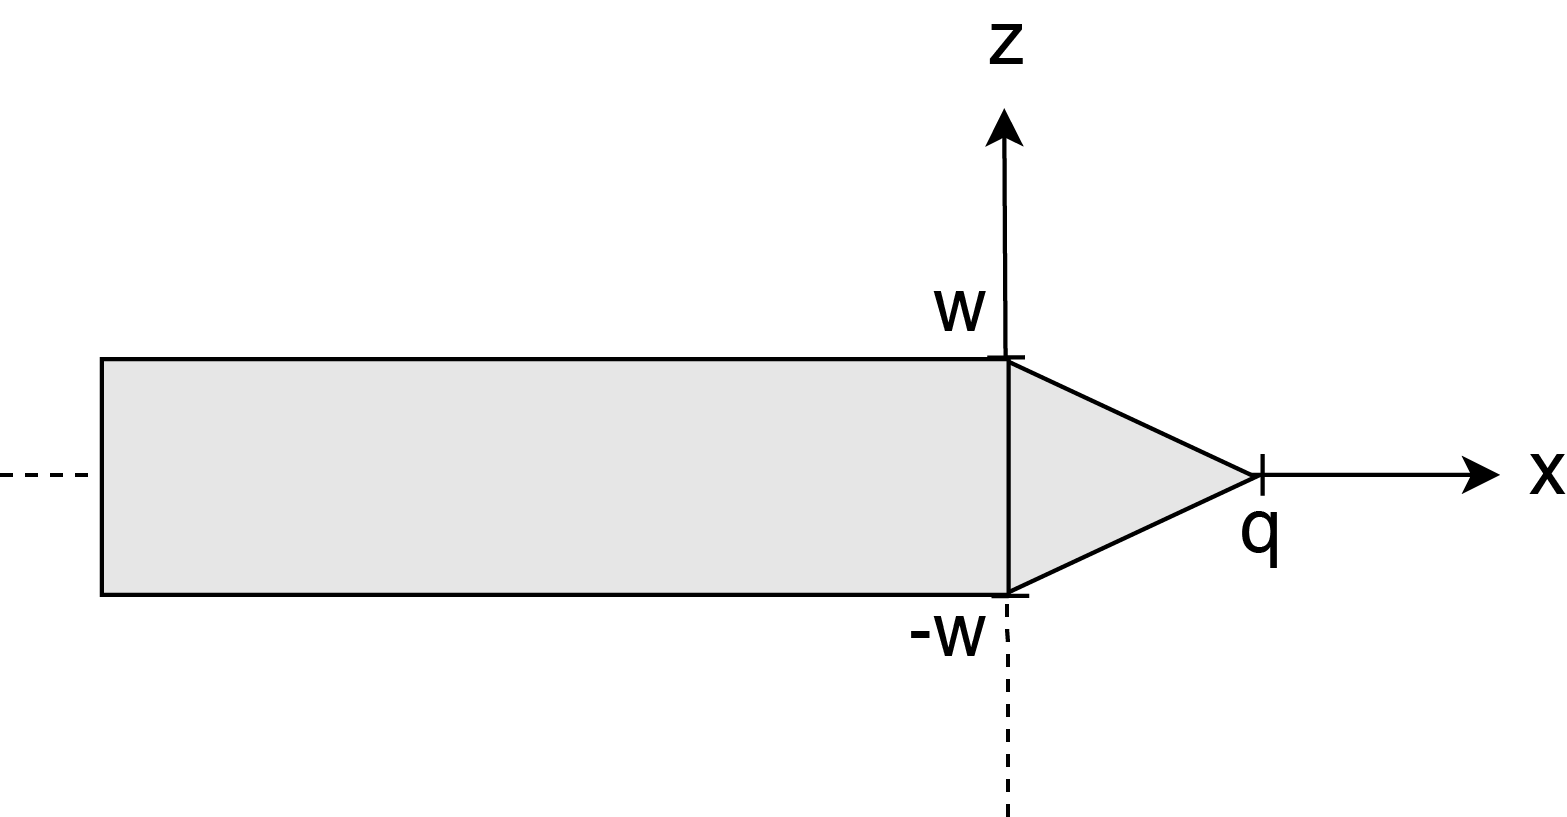
\includegraphics[width=0.4\textwidth]{figures/auv-geo}}
		\captionsetup{justification=centering,margin=2cm}
		\caption{Model of AUV used to calculate the LOS region}
		\label{fig:auv-geo}
	\end{figure}
	
	\item The regions for a $x \leq 0$ are defined as if the hydrophones were flat in the vehicle's surface, which leads to a simplified definition of the LOS region;
	
	\item Since hydrophone $r_1$ is integrated in every configuration, there is no necessity of defining its LOS region.

\end{itemize}

Having these relations into account, the LOS regions are then defined separately for $x \leq 0$ and $x > 0$. When $x \leq 0$, the second simplification previously mentioned is applied so all $ls_i$ are defined as the region greater/less or equal than the tangential to the position of hydrophone $i$ in plane yz. These tangential equations are defined as \ref{eq:los-s2} to \ref{eq:los-s9}.

\begin{eqnarray}
ls_2 \gets x \leq 0 \; \;  \wedge  \; \; z > r_{2_z} \\
\label{eq:los-s2}
ls_3 \gets x \leq 0 \; \;  \wedge  \; \; z < r_{3_z} \\
\label{eq:los-s3}
ls_4\gets x \leq 0 \; \;  \wedge  \; \; y > r_{4_y}  \\
\label{eq:los-s4}
ls_5\gets 	x \leq 0 \; \;  \wedge  \; \; y < r_{5_y} \\
\label{eq:los-s5}
ls_6 \gets	x \leq 0 \; \; \wedge  \; \; z \; \geq \; - y + w \sqrt{2} \\
\label{eq:los-s6}
ls_7 \gets	x \leq 0 \; \; \wedge  \; \; z \; \leq \; y - w \sqrt{2} \\
\label{eq:los-s7}
ls_8 \gets x \leq 0 \; \; \wedge  \; \;  z \; \geq \; y + w \sqrt{2} \\
\label{eq:los-s8}
ls_9 \gets 	x \leq 0 \; \; \wedge  \; \;  z \; \leq \; - y - w \sqrt{2}
\label{eq:los-s9}
\end{eqnarray}

By evaluating these equations, it is possible to infer that the LOS regions for $x \leq 0$ intersect each other, as illustrated in figure \ref{fig:los-color-s0}. The projection is correspondent to the yz plane with an inverted yy axis, in accordance with the previously presented model of the USBL system. Additionally, each colored line corresponds to the LOS region covered by the hydrophone with the same color. For instance, if a transmitter is located in $(-10,-10,-10)$, by analysis of the schematic it is observable that this position is covered by $ls_3$, $ls_5$ and $ls_9$, thus in line of sight of hydrophones 3,5 and 9.

\begin{figure}[!htbp]
	\makebox[\textwidth][c]{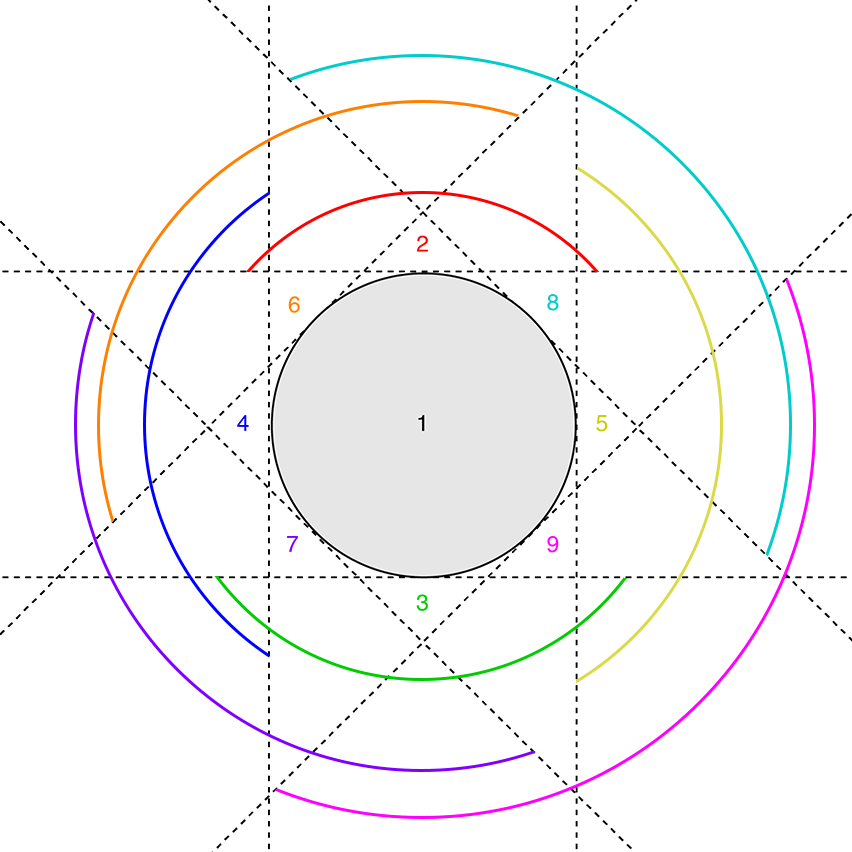
\includegraphics[width=0.6\textwidth]{figures/los-color-regions-back-crop}}
	\captionsetup{justification=centering,margin=2cm}
	\caption{Line of sight regions in plane yz for x < 0}
	\label{fig:los-color-s0}
\end{figure}

Analogously, when $x > 0$, all $ls_i$ are defined as the region greater/less or equal than the tangential to the position of hydrophone $i$ in planes xz or xy, depending on the hydrophone location. Dealing with the hydrophones positioned in the yy and zz axis, $r_2$, $r_3$, $r_4$ and $r_5$, it is possible to directly formulate equations that help defining $ls_2$, $ls_3$, $ls_4$ and $ls_5$ since the tangent plane to these hydrophones is perpendicular to referential planes. However, when considering hydrophones $r_6$, $r_7$, $r_8$ and $r_9$, which are not positioned in any referential axis, the tangential plane which passes through the hydrophone and the front limit of the cone is not parallel to any of the referential planes xy, xz or yz. Therefore, the equations that could define these planes require a rotation of the referential axis. In order to counter this issue, since the shape of the model projected in the yz plane is a circle , if hydrophones $r_6$, $r_7$, $r_8$ and $r_9$ are rotated a $45^{\circ}$ angle around the xx axis, they can become coincident with the positions of $r_2$, $r_4$, $r_5$ and $r_3$ respectively. Additionally, when considering this rotation, the position of the transmitter would also be rotated the same angle to maintain their relative positions. Overall, the used equations are defined by relations \ref{eq:los-b2} to \ref{eq:los-b5}, where the regarded $x,y,z$ coordinates are the original transmitter position for $ls_2$, $ls_3$, $ls_4$, $ls_5$, and the rotated transmitter position for $ls_6$, $ls_7$, $ls_8$, $ls_9$.

\begin{eqnarray}
ls_2, \;  ls_6  \gets x > 0 \; \;  \wedge  \; \; z \geq -\frac{w}{q} x + w  \\
\label{eq:los-b2}
ls_3, \;  ls_9 \gets x > 0 \; \;  \wedge  \; \; z \leq \frac{w}{q} x - w  \\
\label{eq:los-b3}
ls_4, \;  ls_7 \gets x > 0 \; \;  \wedge  \; \; y \geq -\frac{w}{q} x + w   \\
\label{eq:los-b4}
ls_5, \;  ls_8 \gets x > 0 \; \;  \wedge  \; \; y \leq \frac{w}{q} x - w  \\
\label{eq:los-b5}
\end{eqnarray}

After evaluating these equations and the limiting planes that they form, the projected regions of LOS for $r_2$, $r_3$, $r_4$ and $r_5$ are illustrated in \ref{fig:los-color-b0}, where their intersection is evident. The LOS regions of $r_2$, $r_3$, $r_4$ and $r_5$ are naturally similar to these, with an additional rotation of $45^{\circ}$ around the xx axis.

\begin{figure}[!htbp]
	\makebox[\textwidth][c]{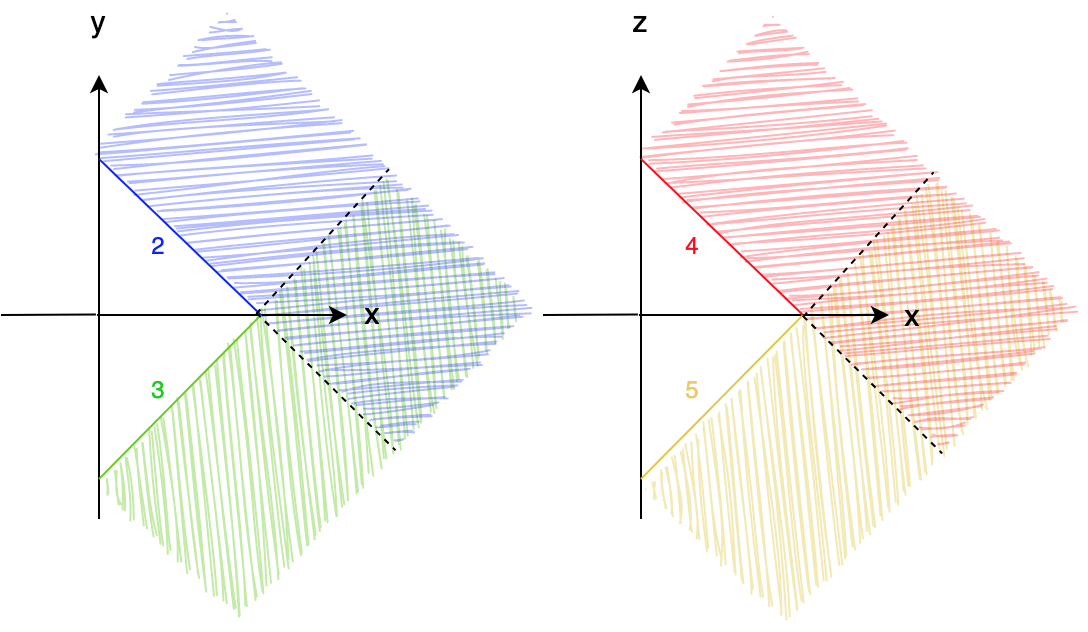
\includegraphics[width=0.7\textwidth]{figures/projections-los}}
	\captionsetup{justification=centering,margin=2cm}
	\caption{Line of sight regions in plane yz for x $\geq$ 0}
	\label{fig:los-color-b0}
\end{figure}

In summary, it is possible to deduce that there are a larger quantity of different configurations that cover the space for $x>0$ than for $x \leq 0$ due to the model of the AUV and the considerations described in the course of this subsection. Therefore it is expected a better estimation for positions of the acoustic source with an azimuth angle between $-90^{\circ}$ and $90^{\circ}$.
%-------------------------------------------------------------------------
%\subsection{Limitations of the system}

%- considerations of the line of sight (mathematical approximations) - line of sight has to be defined for the model considered; if format changes, it has to be remade
%-------------------------------------------------------------------------
\subsection{Simulation results}

\note{add real estimations and findings of best configurations\\
	take a position and calculate best configuration and try to justify why it can be; show second  and third best and explain the difference is/is not substantial}

For the purpose of demonstrating the functionality of the implemented system, various acoustic source positions were tested and the results analyzed.

The first demonstration evaluates the achieved MSE, azimuth deviation and elevation deviation for $s(10,10,10)$. After simulating, plot \ref{fig:errors-101010} compiles the results, where the obtained parametric errors are illustrated for each of the 56 formulated configurations. Additionally, the configurations which are marked with a red circle are the ones whose hydrophones all have full line of sight to the transmitter and the green star indicates which is the configuration that achieves the lowest error. The results of this experiment are aggregated in table \ref{tab:montecarlo-best1}. For the present case, the hydrophones considered to have line of sight to the target are $r_2$, $r_4$, $r_6$, $r_7$ and $r_8$. The configuration with lowest MSE and azimuth deviation is number 8, composed by hydrophones $r_1$, $r_2$, $r_4$ and $r_6$, which are the directly closer to the target. The configuration that originates lowest elevation deviation is number 19, composed by $r_1$, $r_2$, $r_7$ and $r_8$, which maximizes the baseline of the sensors with line of sight.

\begin{figure}[!htbp]
	\makebox[\textwidth][c]{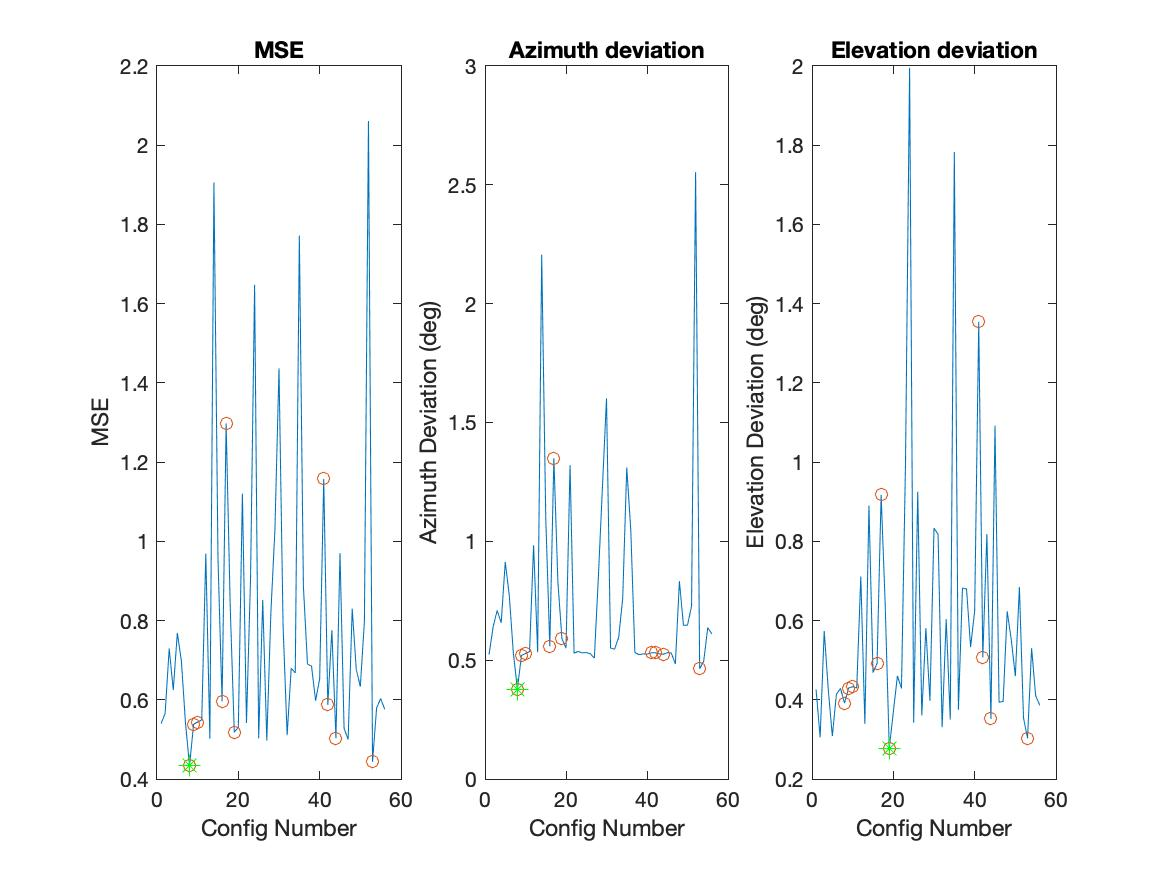
\includegraphics[width=1.1\textwidth,height=0.45\textheight]{figures/plot-[10,10,10]-1000s-errors}}
	\captionsetup{justification=centering,margin=2cm}
	\caption{Errors obtained for all configurations when estimating position (10,10,10)}
	\label{fig:errors-101010}
\end{figure}

Additionally, if the azimuth and elevation deviations are evaluated simultaneously, then the obtained plots can be overlaid to a clear comparison between results. Figure \ref{fig:both-101010} represents this situation where, as the label indicates, the azimuth deviation in degrees is represented by the blue line, the pink line is the elevation deviation in degrees, the red and green circles represent the configurations with line of sight to the target and the green star indicates, once again, the configurations which achieve the minimum deviations in azimuth and elevation. Additionally, the cyan diamond reveals which of the configurations leads to the minimum mean between the azimuth and the elevation deviations. In this case, this corresponds to configuration number 53 which reaches a mean deviation of 0.385 degrees. 

\begin{figure}[!htbp]
	\makebox[\textwidth][c]{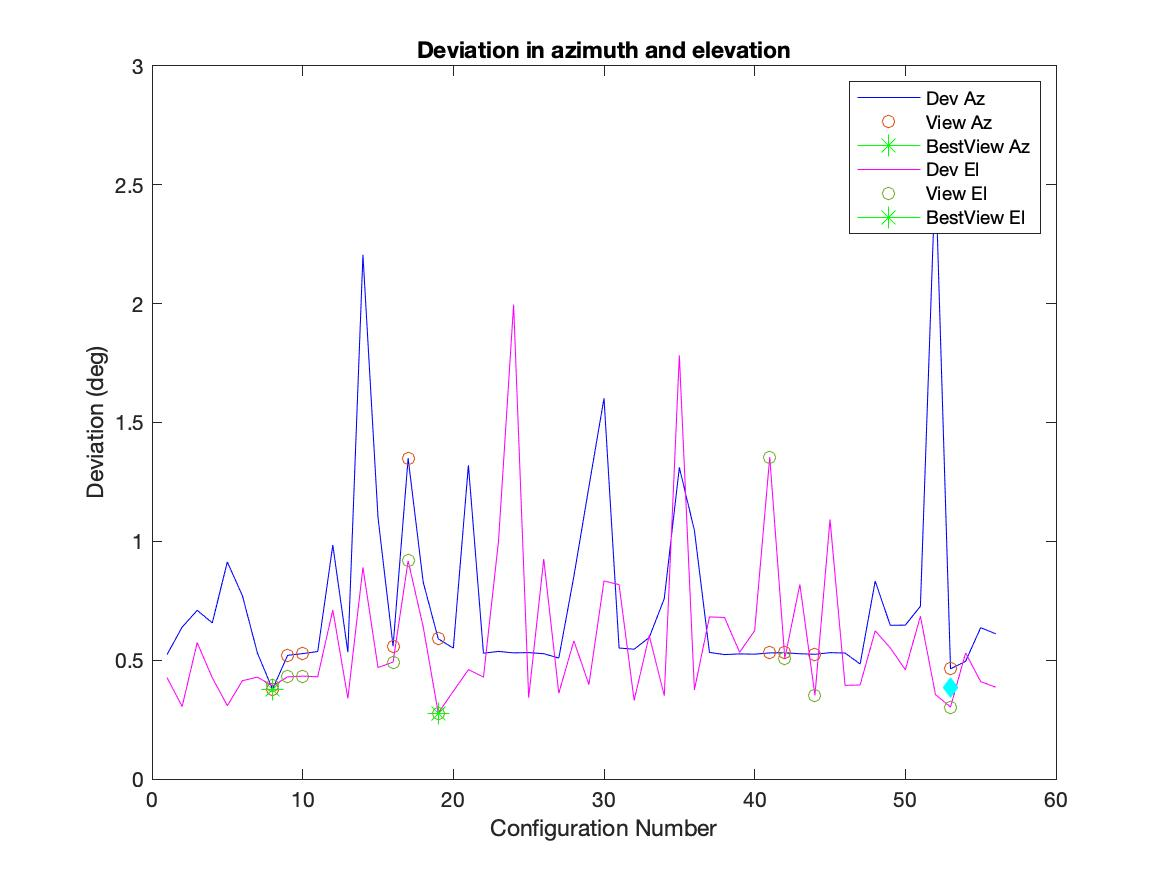
\includegraphics[width=0.9\textwidth]{figures/plot-[10,10,10]-1000s-both}}
	\captionsetup{justification=centering,margin=2cm}
	\caption{Overlaid azimuth and elevation deviations for all configurations when estimating position (10,10,10)}
	\label{fig:both-101010}
\end{figure}

In a second experiment, the position $s(100,100,100)$ is tested, which has the same azimuth and elevation angles as the previous position and a norm 10 times larger. For this case, the error range of azimuth and elevation estimation is approximated the same and the estimation of the norm presents an error approximately 10 times larger. Additionally, as expected the configurations that lead to the lowest errors are the same as for the first experiment.

A set of tests were executed in order to compare the performance of various positions estimation and to extract behavior patterns for the chosen configurations. The collected data is present in table \ref{tab:montecarlo-best1}, where the position of the transmitter is given in Cartesian coordinates by ($s_x$, $s_y$, $s_z$) and for each of the performance parameters it is presented the obtained best configuration number and the minimum error achieved by it. It should also be noted that the notation $0_{+}$/ $0_{-}$ indicates that for a theoretical position with the respective coordinate equal to zero it was returned an estimate which is slightly positive/negative, due to the injected error.


\begin{table}[!htbp] %use H to adjust
	\begin{center}
		\begin{tabular}{ c c c |c c | c c | c c | c c }
			\toprule
			\multicolumn{3}{c|}{} & \multicolumn{2}{c|}{\textbf{Azimuth}} & \multicolumn{2}{c|}{\textbf{Elevation}} & \multicolumn{2}{c|}{\textbf{Azimuth+Elevation}} & \multicolumn{2}{c}{\textbf{MSE}}   \\
			\midrule
			\multicolumn{1}{c}{$s_x$} & $s_y$ & $s_z$ & Config & Min  & Config & Min & Config & Min & Config & Min \\
			\midrule
			\multirow{1}{*}{10} & 10 & 10 & 8 & 0.377 & 19 & 0.278 &  53 & 0.385 & 8  & 0.434\\
			\midrule
			\multirow{1}{*}{-10} & -10 & -10 & 30 & 2.412 & 30 & 1.196 &  30 & 1.804 & 30  & 2.142\\
			\midrule
			\multirow{1}{*}{$0_{+}$} & -10 & -10 & 14 & 2.058 & 14 & 0.431 & 14 & 1.244  & 14  & 1.672 \\
			\midrule
			\multirow{1}{*}{100} & $0_{-}$ & $0_{-}$ & 47 & 0.177 & 32 & 0.177  & 11 & 0.284  & 11  & 0.330 \\
			\midrule
			\multirow{1}{*}{15} & -10 & 5 & 48 & 0.364 & 3 & 0.218 & 27 & 0.346 & 27 & 0.399 \\
			\midrule
			\multirow{1}{*}{$0_{+}$} & $0_{-}$ & 100 & 37 & 52.572  & 39  & 0.381 & 37  & 26.479  & 39 & 32.602 \\
			\bottomrule 
		\end{tabular}
		\caption{Results of Monte Carlo simulation}
		\label{tab:montecarlo-best1}
	\end{center}
\end{table}

Some conclusions can be taken upon the analysis of these results: 
\begin{itemize}
	\item The configurations that achieve the overall minimum errors tend to integrate the LOS hydrophones that attain the larger baseline between them;
	
	\item Transmitter positions that return a higher number of LOS hydrophones, have more possible configurations to choose from and therefore can be more optimized, presenting the lowest errors;
		
	\item The points directly behind the AUV that cover positions with $y$ and $z$ in the range [-w,w], are not contained in any line of sight region;
	
	\item When the transmitter positions have $x \leq 0$, they are in line of sight of less hydrophones than for $x > 0$, so there are fewer possible configurations and the returned best option for the various parameters are more consistent. Consequently, the returned minimum errors are usually higher than for $x > 0$;
	
	\item Transmitter positions that are located near the yy axis, almost in parallel with the circle of hydrophones, are usually covered by only four LOS regions, which correspond to the sensors that are directly closer to the target;
	
	\item For elevation angles close to $90^{\circ}$ and $-90^{\circ}$, the azimuth deviation is much larger than at any other position as expected, since in that region the azimuth angle is more influenced by the injected errors leading to increased deviations.

\subsection{Optimal solution based on range}

After having a comprehensive understanding on the system that is capable of determining which is the best configuration of hydrophones to estimate a specific transmitter position, an alternate scenario can be explored. We now consider that the USBL system does not reconfigure which sensor configuration it should use in order to optimize the estimation  in real time. Instead, a performance study is conducted beforehand so that only two configurations are chosen to be deployed, corresponding to the ones which return the average best estimation of short and long range positions. This way, it would be possible to alternate which configuration is used depending solely on the distance to the target. Alternatively, it is also possible to define just one overall best configuration, in cases where there is the necessity of reducing the number of deployed hydrophones or if the obtained configurations do not have a significant difference in performance.

For the development of this mechanism, there are some adjustments and similarities from the conditions established in the previous system. Firstly, it is assumed that the hydrophones are implemented in a structure shaped like an AUV with no physical form, thus all hydrophone positions have line of sight to any point in space. Additionally, the possibilities for the hydrophone locations are increased for a more extensive study. In order to simplify the arrangement of possible configurations, once again hydrophone $r_1$ is integrated in all configurations and a total of 24 possibilities are considered for the remnant three. These include the same 8 positions $r_2$ to $r_9$, established for the initial setup, to which are added positions $r_10$ to $r_25$ defined in table \ref{tab:config-25h}. This addition corresponds to two replicated circles from the initial one, that assume the same $y$ and $z$ coordinates but are deviated from each other a $d\_x$ equal to 20 centimeters. Figure \ref{fig:24h-config} illustrates all the considered possible positions for the hydrophone's deployment. Accordingly, the number of possibilities is not correspondent to combinations of three out of 24, $C(24,3)$, since these contain linearly dependent configurations when there are hydrophones' positions that only differ in the $x$ coordinate. Therefore, the total number of available combinations is 1512.

\begin{table}[!htbp] %use H to adjust
	\begin{center}
		\makebox[\textwidth]{%
		\begin{tabular}{c | c c c c c c c c c c c c c c c c}
			\toprule
			& r10 & r11 & r12 & r13	& r14 & r15 & r16 & r17	& r18 & r19 & r20 & r21 & r22 & r23 & r24 & r25 \\ \midrule 
			\multirow{1}{0.5em}{x} 
			& 0 & 0 & 0 & 0 & 0 & 0 & 0 & 0 
			& $d\_x$ & $d\_x$ & $d\_x$ & $d\_x$ & $d\_x$ & $d\_x$ & $d\_x$ & $d\_x$\\
			\midrule 
			\multirow{1}{0.5em}{y} 
			& 0 & 0 & w & -w & e & e & -e & -e
			& 0 & 0 & w & -w & e & e & -e & -e\\
			\hline 
			\multirow{1}{0.5em}{z} 
			& w & -w & 0 & 0 & e & -e & e & -e
			& w & -w & 0 & 0 & e & -e & e & -e \\
			\bottomrule 
		\end{tabular}}
		\caption{Additional coordinates for an implementation with 25 hydrophones}
		\label{tab:config-25h}
	\end{center}
\end{table}

\begin{figure}[!htbp]
	\makebox[\textwidth][c]{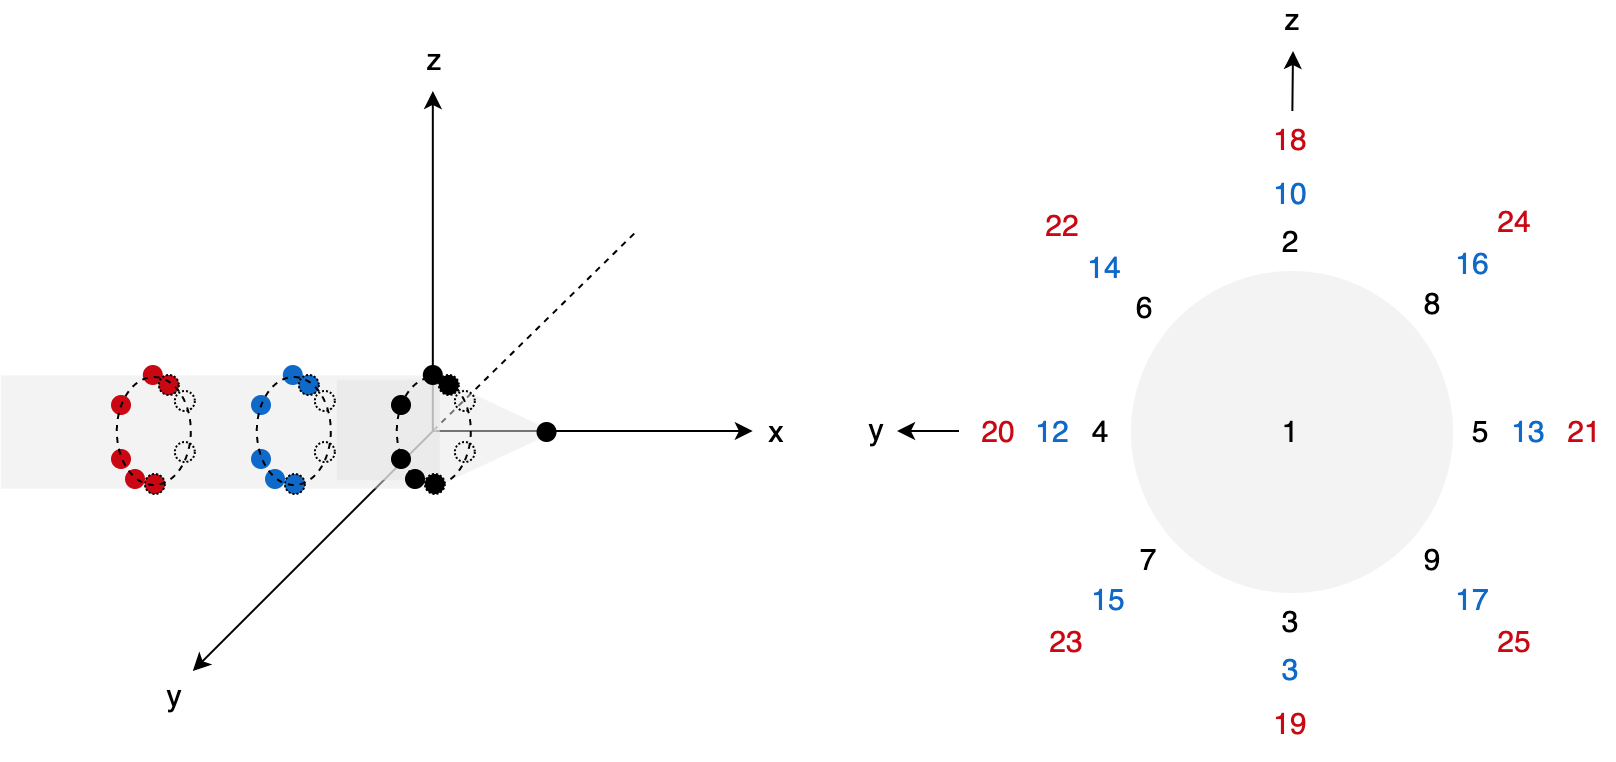
\includegraphics[width=0.9\textwidth]{figures/24h-config}}
	\captionsetup{justification=centering,margin=2cm}
	\caption{Hydrophone possible positions for optimality study based on range}
	\label{fig:24h-config}
\end{figure}

The applied algorithm is similar to the previously explained algorithms \ref{alg:alg1} and \ref{alg:alg2}, with the following variations:

\begin{enumerate}
	\item Similarly to the condition described in \ref{subchap:precision-analy}, the acoustic source positions, $s$, to be estimated are defined in spherical coordinates, where for each defined norm, the elevation component covers the interval [-90$^{\circ}$ to 90$^{\circ}$] in steps of one and, for each elevation value, the azimuth component covers the interval [-180$^{\circ}$, 180$^{\circ}$] in steps of one, forming partial spheres around the reference axis' origin. The norm covers a range between 1 and 10000 meters.
	
	\item An additional logical loop is added in algorithm \ref{alg:alg1} between lines 1 and 2, so that for each possible configuration all $s$ are estimated a number of $i = 1000$ iterations.
	
	\item the $line\_of\_sight$ function is no longer used, as it is considered that all hydrophones have line of sight to every position $s$.
\end{enumerate}

From here it is possible to analyze which are the best returned configurations, according to the chosen parameters MSE, azimuth deviation, elevation deviation and combined azimuth and elevation deviations. According to the numeric errors that are obtained, it is then possible to decide whether there is a single configuration that has evidently a better performance than the others or if there is a pair of configurations that can be used to obtain individually better estimations for short and long range.

\subsubsection{Simulation results}


\end{itemize}

\section{Systematic comparison of geometric configurations performance} \label{sec:analysis_config_performance}

One of the aspects that can be studied to improve the localization estimation is analyzing the best sensor configuration that could be used for a certain scenario. Therefore, it was used the Crámer-Rao lower bound method to do a systematic study on the performance of several hydrophone configurations to be applied in many situations. The study serves as decision method for sensor configurations both applied in an AUV or in a situation without a vehicle. 

The fundamental thought process and mathematical notation used in \ref{sec:cramer} are applied in the study that will be explained next.

\subsection{Crámer-Rao bound}  

Following the logical approach for the process, there are three essential steps that can be differentiated:

\begin{enumerate}
	
	\item Formulate the observations vector
	\item Calculate the Fisher Information Matrix (FIM)
	\item Calculate the determinant of FIM and draw conclusions
	
\end{enumerate}

In this thesis, the number of used hydrophones per estimation is four, so all calculations will be presented for this specific case.

Firstly, the observations vector is formulated based on an initial time of arrival $t_0$, which is given by a synchrony mechanism integrated in the global communication system, and the time-of-arrival based on the vectors that connect the hydrophone positions, $r_i$, to the considered source, $s_t$. For a more realistic approach, it is also considered an added noise component that can be approximated to to a Gaussian distribution $n_i \sim \mathcal{N}(\mu,\,\sigma^{2})$. 

The four observations vector are then formulated as expressed in \ref{eq:obs-my}.

\begin{eqnarray}
t_1 = t_0 + \frac{s_t - r_1}{c} + n_i \\
t_2 = t_0 + \frac{s_t - r_2}{c} + n_i \\
t_3 = t_0 + \frac{s_t - r_3}{c} + n_i \\
t_4 = t_0 + \frac{s_t - r_4}{c} + n_i \\
\label{eq:obs-my}
\end{eqnarray}

Then, addressing the second step, all conditions are set to calculate the FIM,  $I(d) \in \mathbb{R}^{3x3}$. In order to do so, if it is considered d$_{i}$ = $|| s_{t} - r_{i} ||$ as the distance between each sensor and the source, the gradient of the observations vector can be expressed as shown in \ref{eq:grad_fisher}.

\begin{eqnarray}
\nabla_{d}t(d) = \frac{1}{c} 
\begin{bmatrix}
\frac{d_1^T}{||d_1||} \\ 
\addlinespace
\frac{d_2^T}{||d_2||} \\
\vdots \\
\addlinespace
\frac{d_N^T}{||d_N||}
\end{bmatrix}
\label{eq:grad_fisher}
\end{eqnarray}

Additionally, the added noise component which is introduces to the calculations is present in the covariance matrix used in the FIM equation, which is represented as in \ref{eq:covariance}.

\begin{eqnarray}
& \Sigma = 
\begin{bmatrix}
\sigma_1^2 & 0 & 0 & 0 \\
0 & \sigma_2^2 & 0 & 0 \\
0 & 0  & \sigma_3^2  & 0 \\
0 & 0 & 0 & \sigma_4^2 
\end{bmatrix}
\label{eq:covariance}
\end{eqnarray}

Overall, the conditions to obtain the FIM matrix are established and, after some mathematical formulation, it is expressed as \ref{eq:final-fisher}. This expression can be validated by a similar study made on TOA based optimal positioning \cite{cramer-bruno}.

\begin{eqnarray}
I(d) = \frac{1}{c^2} 
\begin{bmatrix}
\sum_{n=1}^{N} \frac{d_i d_i^T}{||d_i||^2} \frac{1}{\sigma_i^2}\\
\end{bmatrix}
\label{eq:final-fisher}
\end{eqnarray}

The final step is to calculate the determinant and find its relation to the volume of the \textit{uncertainty ellipsoid}. As mentioned before, in \ref{sec:cramer}, the determinant of the Fisher Information matrix gives a deterministic value that represents the quantity of information that we can obtain and, therefore, the objective is to maximize it, by respecting the condition $argmax \; det(I(d))$, and consequently minimizing the volume of the ellipsoid. 

\subsubsection{Uncertainty Sphere}

Firstly, it is necessary to choose a set of hydrophone configurations to be tested by the developed simulation environment. Therefore, considering the geometry of an AUV it was formulated a matrix containing nine hydrophones, from which are chosen four at a time to compose the configuration. 

In order to evaluate the obtained determinant values, a way to give physical meaning to this result is to analyze it through the uncertainty volume. However, in an initial approach the ellipsoid was not considered and instead an uncertainty sphere was analyzed. The radius of the uncertainty sphere, $us$, is expressed as \ref{eq:det-sphere}, which translates the three ellipsoid axis into a single mean radius that originates a figure of the same volume.

\begin{eqnarray}
& u_{sphere}(d) = \sqrt[2]{\sqrt[3]{det(I(d)^{-1})}}
\label{eq:det-sphere}
\end{eqnarray}

By doing this, we know are looking to find the $argmin ur(d)$ which indicates that the error that originates that uncertainty radius is minimal.

\subsubsection{Uncertainty Ellipsoid}

\note{eigenvalues give the length of each axis of ellipsoid}

\begin{eqnarray}
& u_{ellipsoid}(d) = \sqrt[2]{eig(I(d)^{-1})}
\label{eq:det-ellip}
\end{eqnarray}


\subsection{Comparison with Monte Carlo simulation}

All the concepts and notions before mentioned were applied in a simulated series of scenarios, where it is attempted to take conclusions about optimal positioning of the sensors for performance improvement. As such, the conditions of the simulation as well as the results of the study are hereinafter explained.

As mentioned before, the key to evaluate the performance when adopting this method is to analyze the determinant of the inverted FIM or, alternatively, the matrix's eigenvalues.

%\begin{figure}[!htbp]
%	\centering
%	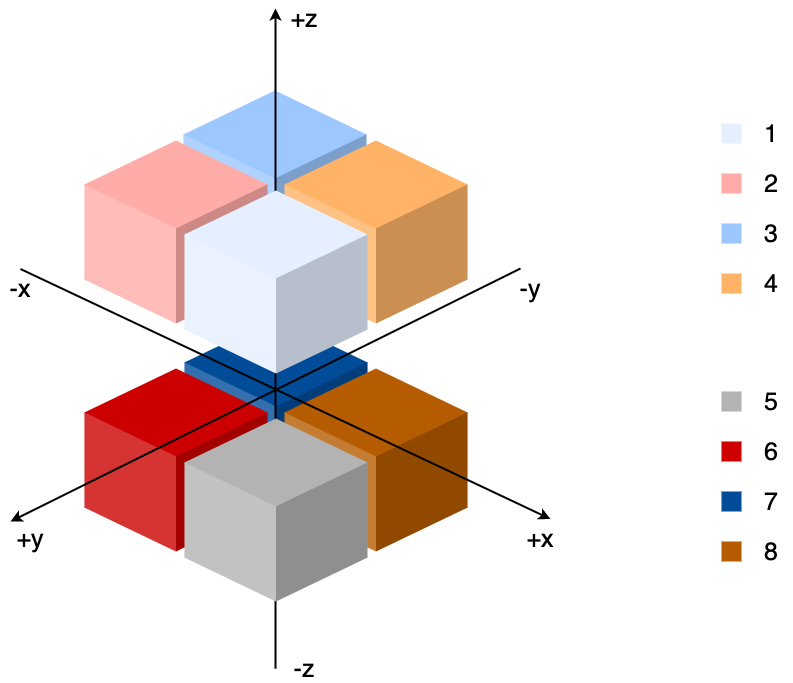
\includegraphics[width=0.7\textwidth]{figures/octant}
%	\caption{Octant discrimination in 3D space}
%	\label{fig:octant}
%\end{figure}



... Layout some results ... 
\\
Ideias:
\\
1-----
\\
- tabela que para cada posição de 4 hidrofones, indica:
\\
- raio de incerteza maximo e posição no espaço onde ocorreu
\\
-raio de incerteza minimo e posição no espaço onde ocorreu
\\
- desvio padrao de todos os pontos no espaço
\\
- uncertainty ellipsoid 
\\
\\
2-----
\\
plot do raio de incerteza para todas as posições no espaço de uma certa configuração

\note{plot da nuvem de pontos e eigen vectors sobrepostos}
\note{comparar best configuration for short and long range}

\note{analyze plane wavefront solution for estimator somwhere}

\section{Conclusions}

\note{-planar wavefront is more simillar to cramer rao for long range source position estimation (discards the non linear components as cramer rao, has some limitations)\\
- cramer rao and monte carlo give different results because my estimator contains non linear components} 

%% Comment next 2 commands if numbered appendices are not used
\appendix
\chapter{Lorem Ipsum} \label{ap1:Lorem}

Depois das conclusões e antes das referências bibliográficas,
apresenta-se neste anexo numerado o texto usado para preencher a
dissertação.

\section{O que é o \emph{Lorem Ipsum}?}

\emph{\textbf{Lorem Ipsum}} is simply dummy text of the printing and
typesetting industry. Lorem Ipsum has been the industry's standard
dummy text ever since the 1500s, when an unknown printer took a galley
of type and scrambled it to make a type specimen book. It has survived
not only five centuries, but also the leap into electronic
typesetting, remaining essentially unchanged. It was popularised in
the 1960s with the release of Letraset sheets containing Lorem Ipsum
passages, and more recently with desktop publishing software like
Aldus PageMaker including versions of Lorem Ipsum~\citep{kn:Lip08}. 

\section{De onde Vem o Lorem?}

Contrary to popular belief, Lorem Ipsum is not simply random text. It
has roots in a piece of classical Latin literature from 45 BC, making
it over 2000 years old. Richard McClintock, a Latin professor at
Hampden-Sydney College in Virginia, looked up one of the more obscure
Latin words, consectetur, from a Lorem Ipsum passage, and going
through the cites of the word in classical literature, discovered the
undoubtable source. Lorem Ipsum comes from sections 1.10.32 and
1.10.33 of ``de Finibus Bonorum et Malorum'' (The Extremes of Good and
Evil) by Cicero, written in 45 BC. This book is a treatise on the
theory of ethics, very popular during the Renaissance. The first line
of Lorem Ipsum, ``Lorem ipsum dolor sit amet\ldots'', comes from a line in
section 1.10.32.

The standard chunk of Lorem Ipsum used since the 1500s is reproduced
below for those interested. Sections 1.10.32 and 1.10.33 from ``de
Finibus Bonorum et Malorum'' by Cicero are also reproduced in their
exact original form, accompanied by English versions from the 1914
translation by H. Rackham.

\section{Porque se usa o Lorem?}

It is a long established fact that a reader will be distracted by the
readable content of a page when looking at its layout. The point of
using Lorem Ipsum is that it has a more-or-less normal distribution of
letters, as opposed to using ``Content here, content here'', making it
look like readable English. Many desktop publishing packages and web
page editors now use Lorem Ipsum as their default model text, and a
search for ``lorem ipsum'' will uncover many web sites still in their
infancy. Various versions have evolved over the years, sometimes by
accident, sometimes on purpose (injected humour and the like). 

\section{Onde se Podem Encontrar Exemplos?}

There are many variations of passages of Lorem Ipsum available, but
the majority have suffered alteration in some form, by injected
humour, or randomised words which don't look even slightly
believable. If you are going to use a passage of Lorem Ipsum, you need
to be sure there isn't anything embarrassing hidden in the middle of
text. All the Lorem Ipsum generators on the Internet tend to repeat
predefined chunks as necessary, making this the first true generator
on the Internet. It uses a dictionary of over 200 Latin words,
combined with a handful of model sentence structures, to generate
Lorem Ipsum which looks reasonable. The generated Lorem Ipsum is
therefore always free from repetition, injected humour, or
non-characteristic words etc. 


%%----------------------------------------
%% Final materials
%%----------------------------------------

%% Bibliography
%% Comment the next command if BibTeX file not used, 
%% Assumes that bibliography is in ``myrefs.bib''
\PrintBib{myrefs}

%% Index
%% Uncomment next command if index is required, 
%% don't forget to run ``makeindex tese'' command
%\PrintIndex

\end{document}
